\documentclass[a4paper,11pt]{article}
%\usepackage[utf8]{inputenc}

\usepackage{amsmath, amsfonts, amsthm, bbm}
\usepackage{dsfont} % to do mathbb{1}
\usepackage{graphicx} 
\usepackage{bmpsize}
\usepackage{tikz}
\usepackage{braket}
\usetikzlibrary{arrows,calc,patterns,decorations.markings,decorations.pathreplacing,plotmarks,shapes.arrows,decorations.pathmorphing,backgrounds}
\tikzset{snake it/.style={decorate, decoration=snake}}
\usepackage[all]{xy}

\usepackage{bm}
\usepackage{hyperref}
\usepackage{float}
\usepackage{titling}
\usepackage{caption}
\usepackage{subcaption}
\usepackage{tikz-cd}
\usepackage{cancel}

\numberwithin{equation}{section}
\theoremstyle{definition}
\newtheorem{definition}{Definition}
\newtheorem{theorem}{Theorem}
\newtheorem{lemma}{Lemma}
\newtheorem{prop}{Proposition}
\newtheorem{comment}{Comment}
\renewcommand{\d}{{\mathrm{d}}}
\newcommand{\e}{{\mathrm{e}}}
\newcommand{\R}{{\mathrm{Ric}}}

\setcounter{tocdepth}{2}
\setlength{\parskip}{3pt}

\title{Quantum energy inequalities with curvature}
\author{Author: Sacha AMIEL \\
Student number: 23126576\\
\\ Supervisor: Dr. Eleni-Alexandra Kontou \\ Module Code: 7CCMTP50}
\date{2024/09}

\usepackage{geometry}
\geometry{a4paper, left=25mm, right=25mm, top=30mm, bottom=25mm}

\renewcommand{\baselinestretch}{1.2}

\begin{document}


\clearpage\maketitle
\thispagestyle{empty}
\begin{figure}[H]
    \centering
    \vspace{100mm}
    
\includegraphics[width=0.2\columnwidth]{Template/kcl_logo.png}
\end{figure}

\newpage
\section*{Abstract}
This project will be, as explicitly stated in the title, about quantum energy inequalities with curvature. It will consist in a formal introduction to an axiomatic approach to quantum field theory, followed by an introduction to energy inequalities and will finish with the beginning of an explicit computation of one of them.

Quantum Energy Inequalities are covariant lower bounds on the energy of a given physics. They do not tell us much about the physics itself, nor about the spacetime the physics unfolds; but from the restrictions they impose on energy, one can (if following general relativity) impose restrictions on that spacetime. This can bring crucial insight in the field of quantum field theory in curved spaces, and therefore, potentially quantum gravity.

\section*{Informal introduction}
It is commonly known in physics that ``energy should be positive", although the more one thinks about it, the less one is sure about it. In the life of a physics student, many formal statements are learned, ``energy is defined up to a constant", ``energy needs to be bounded from below", ``energy is mass so it cannot be negative", ``energy is the curvature of spacetime"... And overall, with time, one gets very flexible with what one can accept as an energy.

In this project we will take the approach of mathematical physics, striving to only work with rigorously well-defined concept. This will lead to results that are less impressive but probably more meaningful. Indeed, the point of quantum energy inequalities is not to claim any result about quantum gravity, but simply to exclude some types of spacetime if one desires to build a physical model with both gravity and quantum field theory. 

\addtocounter{section}{-1}
\section{Introduction}
One of the current ``à la mode" questions in theoretical physics is to find quantum gravity, which is to say, a quantum-field-theory-compatible theory of gravitation that matches all current factual knowledge of our universe and produces observable new predictions.
Let us say it before anything else, the present work will not, in any way, get even remotely close to this extremely complicated task. Several attempts have already been made by many by many people, some which have failed, others which people are still working on, but all of which we will not even mention here. 
We will, on the contrary, take the opposite direction of theoretical physics: that of mathematical physics.

Theoretical physics, by definition, is the art of attempting to guess what new modification one could do to our current understanding of nature in order to improve that very understanding. Mathematical physics, on the other hand, takes for granted (as axioms) the knowledge acquired by theoretical physics (i.e. accepted \emph{theories} of physics) and tries to expand our knowledge of those very same theories without changing them in the slightest. Famous examples of works in theoretical physics could be: Newton's \textit{Law of Motion}; theory of the \textit{Propagation of Heat}; theory of \textit{Classical Quantum Mechanics}. Corresponding mathematical physics work could thus be \textit{Lagrangian} mechanics, \textit{Hamiltonian} mechanics and \textit{Dynamical Systems}; theory of \textit{Fourier} transforms or other systems of wave propagation; theory of \textit{Hilbert Spaces}.

Now, back to the subject at hand, what are theories of physics we will take as our axioms? Those will be theory of \textit{General Relativity} (or ``GR") and that of \textit{Quantum Field Theory} (or ``QFT"). But already, two issues show up. The first one is that the latter of those two theories does not have a rigorous mathematically axiomatized construction accepted by all. That is easily solved though, we will simply choose a particular axiomatization which, to our knowledge, works well, and then, stick to it\footnote{This axiomatization is called \textit{Algebraic Quantum Field Theory}. More on that later.}. The second, and most problematic, is that QFT and GR are two significantly different theories, thus, one cannot candidly ``consider" the two all at once. We will thus be very cautious, when joining them to make the following distinction: we will study a QFT on spacetime first, and then possibly have that spacetime follow the laws of general relativity. How to do so will, of course, be presented to the reader before anything else.

All this being said, now that we know that we do mathematical physics, by accepting particular theories, and extracting new knowledge only from them, comes the question of what new knowledge we seek. As QFT is reasonably well understood on its own, and so is GR, but not quantum gravity itself, we will aim at getting information that restraint how gravity can react to quantum effects, regardless of what \textit{true} quantum gravity can be, rather than trying to actually get a proper GR result. This approach of \textit{restraining} the outputs GR can yield have already been used by R. Penrose in classical GR, using singularity theorems. 

Singularity theorems, given a particular bound on the energy distribution of a manifold, tell us that there exists singularities or event horizons on that manifold. In a way, they allow to ensure the existence of black holes without having to find them. If we were to have such energy bounds for a QFT, we would, consequently, be doing the same it the quantum case. This is what \textit{quantum energy inequalities with curvatures} are. This is the title of this project. We will be explaining generally what they are in detail, and also work on a particular example, called the \textit{Double Smeared Null Energy Inequality}. Although we have not succeeded in fully computing that inequality in time, we have done quite a significant amount of work (and will give the details of what remains to be done to finish that computation, and also how to use this inequality in the future to hopefully get a corresponding singularity theorem).

Being a mathematical physics project, we will heavily rely on some non-trivial mathematical concepts, some of which (like foliation, category theory, or distribution theory) may not be familiar to some. If one wishes to find a rigorous mathematical presentation of what they are (to follow all the details of this project) they are introduced in the \textit{mathematics appendix} on page \pageref{AnMaCat}. But if one solely wants to understand their \textit{physical interpretation} in order to have an intuitive understanding of what they are, that is done separately in the \textit{physics appendix} on page \pageref{AnPhCat}. Either way, whenever new vocabulary from one of these fields is first used, a footnote will indicate where to find it in the appendix, so as to allow as smooth a reading as possible to any reader, regardless of conceptual prerequisites.


\newpage
\tableofcontents
\newpage
\section{Defining Quantum Field Theory in Curved Spacetimes}
This section will make use (without defining them) of notions of \textbf{category theory}. If the reader feels the need for a mathematical definition of what a category is, it can be found on page \pageref{AnMaCat}, in the Mathematics appendices. If the reader feels the need for a physical understanding of what a category is, it can be found on page \pageref{AnPhCat}, in the Physics appendices.

This section will make use (without defining them) of notions of \textbf{distribution theory}. If the reader feels the need for a mathematical definition of what a distribution is, it can be found on page \pageref{DistribMath}, in the Mathematics appendices. If the reader feels the need for a physical understanding of what a distribution is, it can be found on page \pageref{DistribPhy}, in the Physics appendices.

In this section, we will use the symbol $\mathbb{M}_4$ to refer to Minkowski spacetime in 1+3 dimensions, and $\mathcal{M}$ will denote any spacetime with signature $(\mp, \pm,\pm, ..., \pm)$. Any other\footnote{Other than standard undergrad ones (which we assume the reader is familiar with), and concepts related to the notion of foliation, (of which an introduction can also be found in the appendix, both in terms of physical interpretation on page \pageref{PhyFoli} or mathematically rigorous notions on page \pageref{MatFoli}).} notations and concepts will be introduced before being used.

\subsection{Axiomatic approach to Algebraic Quantum Field Theory}
\subsubsection{Formalizing the intuitive idea of a QFT}
\begin{definition}[Quantum Mechanics - \emph{Dirac style}]$\quad$

A quantum Mechanics is the data $(\mathbb{H},\mathcal{T})$ of a Hilbert space $\mathbb{H}$ and some \emph{Time evolution principle} $\mathcal{T}$. In pure theory $\mathcal{T}$ could be \emph{any} labelling of \emph{everything} with respect to time, but in practice, it will usually be given by some time-evolution equation on either the vectors of $\mathbb{H}$, the operators of $\mathbb{H}$, or in some very specific cases, both...\\
An example of vector evolution would be, given a Hermitian operator $H\in\mathcal{B}(\mathbb{H})$, the well-known Schrödinger-picture time-evolution:
$$\boxed{\mathcal{T}_{H,\mathrm{Sch}}: \Bigg\{
\begin{matrix}
\mathbb{H} & \to & \mathcal{C}^\infty(\mathbb{R},\mathbb{H})\\
\Psi & \mapsto & \Big(t\mapsto \e^{\mathfrak{i}\hbar H}\Psi\Big)
\end{matrix}}\;.$$

An example of an operator time evolution would be the well-known Heisenberg-picture time-evolution (which, if taken with the same $H$ (Hamiltonian) is \emph{physically equivalent}):
$$\boxed{\mathcal{T}_{H,\mathrm{Hei}}: \Bigg\{
\begin{matrix}
\mathcal{B}(\mathbb{H}) & \to & \mathcal{C}^\infty\big(\mathbb{R},\mathcal{B}(\mathbb{H})\big)\\
X & \mapsto & \Big(t\mapsto \e^{-\mathfrak{i}\hbar H}X\e^{\mathfrak{i}\hbar H}\Big)
\end{matrix}}\;.$$

But some more whimsical time-evolutions can be used, for instance, in several methods of perturbation theory in molecular physics (drawing from a mixture of the previously mentioned ones). In a way, one can also consider the Dirac equation or the Klein-Gordon equations as being other time-evolutions also defining quantum mechanics (though in practice, we want to see them as part of a Quantum Field theory, which is something we will define next).

Note that the definition can often extend all the sets $\mathcal{B}(\mathbb{H})$ to $\mathcal{L}(\mathbb{H})$, i.e. disregard the requirement of boundedness. Although this makes things much harder to define mathematically (exponential of operators suddenly require a bit more work in the definition), the idea remains exactly the same. In what follows we will keep track of this subtle difference, but unless it is of interest to the reader, we suggest not minding it.
\end{definition}

\begin{definition}[States - Observables - and Physically Identical QMs] \emph{vocabulary}


``States" are the set $\mathbb{C}\mathcal{P}_\mathbb{H}$, i.e. the projective space of the Hilbert space of the quantum mechanics. Recall that the projection of a vector space is the set of all equivalence classes $\{\lambda \Psi, \lambda\in\mathbb{C}\}$ for all vectors $\Psi$ in $\mathbb{H}$. In practice, one often confuses (non-zero) vectors of $\mathbb{H}$ with their projection and just calls them states, while keeping in mind that they are identical up to change of norm and phase.

``Observables" are self hermitian operators of $\mathbb{H}$. Or a sub-algebra of it (depending on the context). The physically observable information of a quantum mechanics is the spectrum of these operators. Thus, if two QM yield the same spectra up to an isomorphism of QMs (understand by that an isomorphism of Hilbert spaces AND of time evolution) we say that they are descriptions of the same physical systems, i.e. the same. From a more formal point of view, this is like having a bijective functor on the category of QMs (where Hilbert Spaces are the objects, and time-evolutions are the morphisms).

As mentioned previously, an example of this idea is QMs in the Schrodinger picture and in the Heisenberg picture, which are physically the same when using the same $H$. More trivial cases of two quantum mechanics being the same are for instance when we keep the same time-evolution but replace the Hilbert Space by an isomorphic one (for instance, switching $\mathcal{S}(\mathbb{R}^3)$ with itself using the Fourier Transform, which is called switching from ``momentum representation" to ``position representation" is quite a standard example).    
\end{definition}

\begin{definition}[Quantum Field Theory] \emph{informal definition}

    The broad idea of a quantum field theory (QFT) is that it is sort of a quantum mechanics, but that it is covariant and describes Fields...
    To this day, there is not yet a clear consensus on any proper axiomatic definition; but next we define an \emph{Algebraic Quantum Field Theory} (AQFT), which does fit in this fuzzy idea, and then we will just assume all QFTs to be AQFTs from then on.
\end{definition}
\begin{definition}[C*-Algebra]
    $\quad$
    
    A C*-Algebra is a tuple $(\mathcal{A}, ||\cdot||)$ where:
    \begin{itemize}
        \item $\mathcal{A}$ is a unital (i.e. has a unit) *-Algebra over $\mathbb{C}$;
        \item $||\cdot||$ is a norm over $\mathcal{A}$ as a complex vector space;
        \item $\forall (A,B)\in\mathcal{A}\;\; ||AB||\leq||A||\cdot||B||;$
        \item $\forall A\in\mathcal{A}\;\; ||A^*\; A||=||A^*||\cdot||A||=||A||^2;$
        \item $\mathcal{A}$ is \emph{complete} in the $||\cdot||$-metric topology.
    \end{itemize} 
    
For simplicity, we will always assume that $||\mathds{1}||=1$... That's just the redefinition $||\cdot||\mapsto\frac{||\,\cdot\,||}{||\mathds{1}||}$, so nothing to overthink there...
\end{definition}

\begin{comment}
\label{Com:C*&Bound}
Notice that $\mathcal{B}(\mathbb{H})$ forms a C*-Algebra, using duality ($\dag$) as $*$-operator and operator norm $\left(||A||:=\mathrm{Sup} \left\{\frac{||A\Psi||}{||\Psi||},\Psi \in \mathbb{H}\right\}\right)$ as algebra norm.
\end{comment}

\subsubsection{The axioms of AQFT}
The few following definitions are taken from \cite{AQFT_Intro}. They can also be found in \cite{pAQFT}, but that last one goes a bit further, as we will see in a moment.
\begin{definition}[AQFT] \label{AQFT_M4-Ax}
    An AQFT is a tuple $\big(\mathcal{A}(\mathbb{M}_4), \mathcal{A}(\cdot)\big)$. Where $\mathcal{A}(\mathbb{M}_4)$ is a C*-Algebra and $\mathcal{A}(\cdot)$ is a functor from the category $\mathcal{O}(\mathbb{M}_4)$ of open causally convex subsets of $\mathbb{M}_4$ to that of sub-C*-Algebras of $\mathcal{A}(\mathbb{M}_4)$ obeying the following requirements:
    \begin{enumerate}
        \item \textbf{Locality}:  $\big\{\mathcal{A}(O), O \in \mathcal{O}(\mathbb{M}_4) \; \mathrm{with}\; O\; \mathrm{bounded}\big\}$ generates $\mathcal{A}(\mathbb{M}_4)$;
        \item \textbf{Isotony}: $\forall (O_1, O_2) \in \mathcal{O}(\mathbb{M}_4)^2 \quad O_1\subset O_2 \implies \mathcal{A}(O_1)\subset\mathcal{A}(O_2)$;
        \item \textbf{Causality}: $\forall (O_1, O_2) \in \mathcal{O}(\mathbb{M}_4)^2 \quad O_1 \; \mathrm{and}\; O_2\; \mathrm{causally}\;\mathrm{disjoint}\; \implies \big[\mathcal{A}(O_1),\mathcal{A}(O_2)\big]=0$;
        \item \textbf{Covariance}: there exists a functor $\alpha$ from the category of the (identity connected) Poincaré transformations of $\mathcal{O}(\mathbb{M}_4)$ to that of the sub-C*-Algebras of $\mathcal{A}(\mathbb{M}_4)$;
        \item \textbf{Spectrum Condition}: We require the existence of a representation (see next definition) of the algebra where the translations are unitarily implemented (physically, this means we want translation-invariant physics);
        \item \textbf{Dynamics}: $\forall (O_1, O_2) \in \mathcal{O}(\mathbb{M}_4)^2 \;\;;\mathrm{with} \;\;O_1 \subset O_2$, if $O_1$ contains a \emph{Cauchy Surface}\footnote{In short a Cauchy surface is a surface met once by all geodesics. However, since this is a very important object of AQFT in curved spaces, and since it is also related to foliations which we already mentioned and will extensively use in the last section, we recommend any reader unfamiliar with Cauchy surfaces to check out how they are rigorously defined on page \pageref{CauchyMat} of the Mathematics appendix or at least their physical interpretation on page \pageref{CauchyPhy} of the Physics appendix.} in $O_2$, then $\mathcal{A}(O_1)=\mathcal{A}(O_2)$.
    \end{enumerate}
    
Note that the true definition of an AQFT actually doesn't always use C*-Algebras but sometimes simply *-Algebras (especially when doing perturbation theory). But since dropping the C* requirement makes things a lot more complicated (it's basically like disregarding any topological concerns) when it simply doesn't make false many important results, most researchers in the field focus on C*-AQFT and we will simply ignore the other ones.
\end{definition}

\begin{definition}[States - Observables] \emph{vocabulary of QFT}

"States" are elements $\omega: \mathcal{A}(\mathbb{M}_4)\to\mathbb{C}$ obeying the following properties:
\begin{itemize}
    \item $\forall \lambda\in\mathbb{C}, \forall(A,B)\in\mathcal{A}(\mathbb{M}_4)^2\quad \omega(\lambda A+B)=\lambda \omega(A)+\omega(B)$;
    \item $\forall A \in \mathcal{A}(\mathbb{M}_4)\quad \omega(A^*\, A)\in \mathbb{R}_+$;
    \item $\omega(\mathds{1})=1$.
\end{itemize}
"Observables" are self-adjoint elements of $\mathcal{A}(\mathbb{M}_4)$, i.e. the elements of: $\{A \in\mathcal{A}(\mathbb{M}_4):A=A^*\}$.
\end{definition}

\subsubsection{Relating AQFT to the intuitive ideas of QFT}
\begin{comment}
\label{Com:SymDiracWeyl}
    Recall, from comment \ref{Com:C*&Bound}, that given any Hilbert space $\mathbb{H}$, the bounded operators of it $\mathcal{B}(\mathbb{H})$ forms a C* Algebra.
    
    Notice that, a linear form $\frac{\bra{\Psi}\,\cdot\,\ket{\Psi}}{\braket{\Psi|\Psi}}$ gives us a ``State" in the QFT sense, and that is so for all $\lambda\ket{\Psi}$ corresponding to the same state, the associated linear form will be identical.
    
    All this, (associated to the fact that $\mathbb{M}_4$ can be foliated\footnote{If the reader is unfamiliar with the notion of foliation, it is introduced in the appendix. On page \pageref{MatFoli} of the Mathematics appendix is a formal introduction, and a physical interpretation can be found on page \pageref{PhyFoli} of the Physics Appendix.} with respect to time) sort of hints us towards the idea that AQFT is indeed sort of what a QFT should be (i.e. a covariant QM).
    
    Now, it turns out that, intrinsically, a QFT is not a QM, for some subtle reasons. It would be more rigorous to say that every QFT \emph{contains several QMs}... Let us build up to this more formally.
\end{comment}

\begin{definition}[Representation of a C*-Algebra]$\quad$

    A representation of a C*-Algebra $\mathcal{A}$ is a triple $(\mathbb{H},\mathcal{D},\pi)$ where $\mathbb{H}$ is a Hilbert Space; $\mathcal{D}$ a dense subspace of it; and $\pi : \mathcal{A}\to\mathcal{B}(\mathcal{D})$ a morphism of C*-Algebra such that $\pi(\mathds{1}_{|\mathcal{A}})=\mathds{1}_{|\mathcal{D}}$.
    Unsurprisingly, it will be called a \emph{faithful} representation when $\mathrm{Ker}(\pi)=\{0\}$ and irreducible if without any invariant subspaces...
    
    So from that, it becomes sort of obvious that any representation of the algebra of a QFT, associated with a $\mathcal{T}$ to keep track of the time each subalgebra is from (which is trivially extracted from the $\mathcal{A}$ functor), does indeed lead to a proper QM.
\end{definition}

\begin{comment}
    It turns out that, given a state (a pure state) $\omega$ one can always build a representation that works as broadly teased in comment \ref{Com:SymDiracWeyl} and yields a faithful irreducible representation, with a vector $\ket{\Omega}$ such that $\omega\simeq\bra{\Omega}\cdot\ket{\Omega}$.
    
    And that representation will be unique up to unitary equivalence (i.e. yield exactly the same QM). This is Theorem 10 in \cite{AQFT_Intro}. One can see this particular representation (called GNS representation) as a ``canonical representation" of a QFT associated to a particular state.
\end{comment}

\begin{comment}
    In the case where any two such representations are unitarily equivalent, we see that the given QFT \textbf{\textit{is}} a quantum mechanics... But it turns out many QFTs do not have this property, in particular the algebra of operators of free field theories do not have this property.
    
    This is characterized by the author of \cite{AQFT_Intro} as the intrinsic presense of quantum fields in a theory. All purely QFT statements of the algebraic formulation are written in terms of this study of inequivalent representations. In particular, the structure of all inequivalent reps, formulated with ``superselection sectors" yields what can be seen as algebraic gauge theory...
    
    Gauge theory will not be part of our study, nor will any representation issues. They were only quoted as a way to justify our choice of axioms: all evidence suggests that the mathematical object at hand \emph{is} quantum field theory on $\mathbb{M}_4$. One can now accept it in full confidence, to move into the next step toward quantum energy inequalities.
\end{comment}


    
\subsection{Fields in curved spacetimes}

\subsubsection{Separating the notion of a Field from its spacetime}
Recall that $\mathcal{A}(\cdot)$ can be seen as a covariant functor from the spacetime to the Algebra of observables.
        
Let $\bold{Loc}$ be the category of hyperbolic oriented and time oriented spacetimes related by respective embedding. Let $\bold{Vec}$ be the category of topological vector spaces (with continuous linear functions as morphisms). And let $\bold{Obs}$ be the category of locally convex C*Algebras (or just unital *Algebras in the context of perturbation theory, or topological Poisson Algebras in the classical case) with corresponding algebra morphisms as morphisms. 
Let $\mathcal{D}$ be the functor from $\bold{Loc}$ to $\bold{Vec}$ that associates to every spacetime its compactly supported test functions.

\begin{definition}[Quantum Field]\label{QField}$\quad$

    A Quantum Field is a natural transformation from the functor $\mathcal{D}$ to the functor $\mathcal{A}(\cdot)$ of field theory composed with the forgetful functor from $\bold{Obs}$ to $\bold{Vec}$.\\
    We will detail the meaning of this definition in the next section, do not be frightened by how abstruse this definition looks.
\end{definition}

This definition is abstract enough to hold over any spacetime (as the categories used to not require anything reserved to $\mathbb{M}_4$), this leads us to slightly weaken the axioms of AQFT (called pAQFT) as follows (see \cite{pAQFT} for more), it will, among other things, allow to include perturbation theory to the frame but also make it work on any spacetime.\\
A perturbative quantum field theory over any spacetime is the data $\big(\mathcal{M},\mathcal{A}(\mathcal{M})\big)$ such that:
\begin{itemize}
    \item There is a net to topological *-algebras with sequentially continuous product over a spacetime $\mathcal{M}$; $\mathcal{O}\mapsto\mathcal{A}(\mathcal{O})$ (i.e. the observable functor is well-defined);
    \item \textbf{Locality}, \textbf{Isotony}, \textbf{Causality} and \textbf{Covariance} hold (see definition \ref{AQFT_M4-Ax} for formulae, just replace $\mathbb{M}_4$ with $\mathcal{M}$);
    \item \textbf{Time-slicing axiom}: Algebra of the neighbourhood of a Cauchy surface\footnote{In short a Cauchy surface is a surface met once by all geodesics. However, since this is a vary important object of AQFT in curved spaces, and since it is also related to foliations which we already mentioned and will extensively use in the last section, we recommend any reader unfamiliar with Cauchy surfaces to check out how they are rigorously defined on page \pageref{CauchyMat} of the Mathematics appendix or at least their physical interpretation on page \pageref{CauchyPhy} of the Physics appendix.} of a Region is the algebra of the whole region. (To get a time-evolution);
    \item Notice, however, that the spectrum condition can no longer be used on curved surfaces, as ``translations" are not everywhere well-defined. To not lose this idea of ``translation invariant physics", we will instead, make use of Hadamard states \label{FirstMentionHad}(see Section \ref{DefHad} for details).
\end{itemize}

Although we will not use this definition, but rather an equivalent one, let us, for the sake of rigour, define Hadamard states right now.
\begin{definition}[Wavefront Set]
    Let $u \in \mathcal{D}'(\Omega)$ be a distribution. Its wavefront set, denoted $\mathrm{WF}(u)$ is the complement in $\Omega\times(\mathbb{R}^n\setminus\{0\})$ of the set of points $(x,k_0)$ such that there exists a test function $f \in \mathcal{D}(\Omega): f(x)=1$  such that, for some open conic neighbourhood $C$ of $k_0$
    \begin{equation}
    \forall N \in \mathbb{N} \quad \underset{k\in C}{\mathrm{sup}} \Big((1+|k|)^N \left|\mathcal{FT} \big(f\cdot u(k)\big)\right|\Big) <\infty
    \end{equation}
    where $\mathcal{FT}$ denotes the Fourier transform, though its definition on a manifold is chart-dependent, its boundedness isn't.
    One can, likewise, define a wavefront set for bi-distributions.
\end{definition}
The wavefront set can be seen as the spacetime $\times$ momentum places where the distribution has a well-defined spectrum.
\begin{definition}[Hadamard State]\label{HadDef}
    Denoting by $\Bar{V}_{+,x}$ the closed future cone at spacetime point $x$, and by $(x,k)\sim(x',k')$ the equivalence relation ``there exists a null geodesic strip containing the two pairs". One calls \emph{Hadamard} a state whose two-point-function $W$ has the following properties:
    \begin{itemize}
        \item $W$ is a bi-solution of the equations of motions
        \item $W$ is positive definite
        \item $\mathrm{WF}(W)=\{ ((x,k),(x',-k'))\in \mathrm{T}^*\mathcal{M}^2 : (x,k)\sim(x',k')\wedge k \in \Bar{V}_{+,x}$
    \end{itemize}
\end{definition}
The physical interpretation of a Hadamard state is thus that not only is the state physical (equation of motion and positiveness) but so is its spectrum (which needs to be bonded by the causal structure of the spacetime, no more, no less).

\begin{comment} \label{QFT+GR}
    Once this is our definition of QFT on curved spacetimes, we can look back at our definition of fields. It was formulated exclusively in terms of $\mathcal{A}$ and geometrical categories (\textbf{Loc}, \text{Obs}, ect...) and categories are only structural requirements. This means that \emph{for the same field} we can consider \emph{different spacetimes}. Doing this is too abstract to have some experimental meaning (which is to be expected, as we are still at the functor level), but having the freedom to change spacetime at will is the key ingredient of General Relativity, hence, just like Einstein in his time, we can now ask formal questions about the spacetime \emph{given} a field.
    This, of course, will not be quantum gravity, but we can get close enough to formally impose Einstein's equation on the spacetime, thereby doing what some call effective quantum gravity. Or, in more down to earth words, this is not quantum gravity, but the response of classical gravity to quantum field theory.\\
\end{comment}

We have now entered the final mathematical framework to study quantum energy conditions. It required a considerable amount of abstraction, to the point where, it is natural for one to be lost, especially if one is familiar with the way QFT is historically thought (i.e. not like that at all). Let us now go back to the definition of a field and get to a practical understanding of it.
\subsubsection{Understanding the over-complicated definition of a Field}
Recall definition \ref{QField}, and let us build to an understanding of it:
\begin{center}
    A Quantum Field is a natural transformation from the functor $\mathcal{D}$ to the functor\\ $\mathcal{A}(\cdot)$ of field theory composed with the forgetful functor from $\bold{Obs}$ to $\bold{Vec}$.
\end{center}
\textbf{Obs} are physical observables (i.e. *Algebras). \textbf{Vec} are vector spaces. As one knows, any algebra is a vector space (by their respective definitions). What we call the \emph{forgetful} functor is thus the fact of ignoring the product of an algebra. Thus ``the forgetful functor from $\bold{Obs}$ to $\bold{Vec}$" means ``disregarding the product of operators".\\

$\mathcal{D}$ is the functor that associates to every area of spacetime a ``test function\footnote{See \textit{Distribution Theory} in the appendix for more on these objects.}". Now, a field is defined as a natural transformation from $\mathcal{D}$ to $\mathcal{A}$, so it takes in the test functions (and their spacetime structures) and sends it to the observable, although (in the output) we only get the vector information. So physically, a Field is a non-commutative (i.e. quantum object) that can be probed in spacetime, and whose values will be regular numbers.\\ \\
This does correspond to what is known in QFT as a quantum field.\\

\noindent Here are some easy examples of fields:
\begin{itemize}
    \item The one that just reads the value at a point O of a test function (known as a Dirac $\delta$ distribution).
    \item One can create a family of fields starting from a single one (called $a$) taking its dual ($a^\dag$) and making sure it commutes as such ($[a,a^\dag]=\delta$); $a$ will then be called a ladder operator...
\end{itemize}

A more rigorous mathematical treatment of the definition of the field will lead to the properties of the next sections. (It will also, \emph{finally}, look like the fields physicists are familiar with.)

\subsubsection{Computational properties of a Field}
        \begin{theorem}[Linearity \& Hermicity]$\quad$
        
         For any field $\phi\in\mathcal{D}'(\mathcal{M})$ for any two test functions $f,g\in\mathcal{D}(\mathcal{M})$ and any scalar $\lambda\in\mathbb{C}$  the two following equalities hold:
         \begin{align}
             \phi(\lambda f+ g) &= \lambda\phi(f)+ \phi(g),&
             \phi(f)^\dag &= \phi(f^*).
         \end{align}
        \end{theorem}
        \begin{definition}[On shell fields]$\quad$

        Our algebra of ``physical" (called ``on shell") fields is technically not $\mathcal{D}'(\mathcal{M})$ as we also impose field equations and commutation relations (usually obtained from canonical quantization of an action). This is us making a choice in the previously mentioned natural transformation. Formally, we are given a filed equation $\mathfrak{F}$ and canonical commutation relations $\mathfrak{C}$, and ``on shell" is the algebra $\mathcal{D}'(\mathcal{M})/(\mathfrak{F}\wedge\mathfrak{C})$.

        In practice though, since $\mathcal{D}'(\mathcal{M})/(\mathfrak{F}\wedge\mathfrak{C})$ is isomorphic to a sub algebra of $\mathcal{D}'(\mathcal{M})$ and since the latter is much nicer, we will simply work in $\mathcal{D}'(\mathcal{M})$ and impose that physical fields $\mathcal{D}'_\mathrm{shell}(\mathcal{M})\subset\mathcal{D}'(\mathcal{M})$ have the following extra properties.
        \end{definition}
        
        \begin{theorem}[On shell \& commutation properties]$\quad$
        
        Let $\mathcal{P}$ be our field equation operator and $\mathcal{E}(\cdot,\cdot)$ be our energy\footnote{In fact, to be rigorous, this is the anti-symmetric part of our Hadamard State...} the following equations hold for any $f,g\in\mathcal{D}(\mathcal{M})$:
        \begin{align}
            (\mathcal{P}\phi)(f):=&\phi(\mathcal{P}f)=0, &
            [\phi(f),\phi(g)]=&i\mathcal{E}(f,g)\mathds{1}.
        \end{align}            
        \end{theorem}

\noindent In our case, we will work with the simple Physics derived from the Lagrangian :
        \begin{equation}
        \mathcal{L}=\frac{\sqrt{|g|}}{2}\left(\nabla^\mu\phi\nabla_\mu\phi- (m^2+\xi R)\phi^2\right);
        \end{equation}
        leading to:
        \begin{equation}
        \mathcal{P}:=\square_g + m^2 + \xi R,
        \end{equation}
        where $g$ is the spacetime's metric, $R$ its Ricci curvature, $m$ is a real scalar (mass of the field), $\xi$ a real scalar (gravitation coupling).

        
\subsection{From its axiomatization to its practical implementation}
\subsubsection{Computation-oriented depiction of Fields}
        Now that all these mathematical prerequisites have been dealt with, we will define many useful objects of QFT. Readers familiar with physics will definitely find all the following expression to be identical to what is taught in basic courses, (the only difference being that we now know their mathematical inner working) and that is to be expected as our plan is definitely not to re-invent physics.

        \begin{definition}[Basic Physical Objects in QFT]$\quad$
        \begin{itemize}
            \item \underline{The Action}: $S:= \int \mathcal{L}$ is sort of the cost function of each field configuration (thought that would be a \emph{classical interpretation}).
            \item \underline{Energy Momentum Tensor}: $T_{\mu\nu}:=\frac{2}{\sqrt{|g|}}\frac{\delta}{\delta g^{\mu\nu}}S.$
            \item \underline{Feynman Propagator}: $G^\mathrm{F}(x,x'):=i\bra{\psi}T\Phi(x)\Phi(x')\ket{\psi}$ where $\ket{\psi}$ is a given state, and $T$ is the \emph{time ordering operator} which we will not go into right now. In our calculations, we will only work with $H:=-iG^\mathrm{F}$ which is the real bi-distribution instead (called Hadamard parametric). 
        \end{itemize}
        \end{definition}
        All these are the objects of QFT, but, on their own, they are a bit too general, which is why we restrict ourselves to previously mentioned powerful states called \emph{Hadamard states}.
\subsubsection{Renormalization}
    As mentioned before, the following formulae only work for Hadamard states, we will not state it each time, nor truly explain why as we do not discuss any other types of states. We shall first focus on how to do renormalization in curved spacetimes. 

    The idea behind renormalization is to isolate singularities in QFT. To be precise, (as we haven't encountered any singularity so far) singularities are not present in QFT per say, but they arise as we attempt doing computations at the limit of infinitely far away objects or infinitely close.

    We define a few operators and other objects:\\
    First the parallel propagator on the manifold, that implements parallel transport, $g_{\mu\nu'}(x,x')$ from spacetime point $x'$ to $x$ such that the vector $l^{\nu'}(x')$ is sent to:
    \begin{equation}
    l^{\mu}(x)=:g^\mu_{\nu'}(x,x')l^{\nu'}(x')
    \end{equation}
    naturally, as $x'$ goes to $x$ we recover no transport at all, i.e. just the metric:
    \begin{equation}
    \lim_{x\to x'} g_{\mu\nu'}(x,x')=g_{\mu\nu}(x')
    \end{equation}
    we also have the point-split stress-energy operator (or canonical quantization of the energy momentum tensor), which in our case is:
    \begin{equation}
    \mathbb{T}^\mathrm{split}_{\mu\nu}(x,x'):=\nabla^{(x)}_\mu\otimes\nabla^{(x')}_{\nu'}-\frac{1}{2}g_{\mu\nu'}(x,x')g^{\lambda\rho'}(x,x')\nabla_\lambda^{(x)}\otimes\nabla_{\rho'}^{(x')}+\frac{1}{2}m^2g_{\mu\nu'}(x,x')1\otimes 1
    \end{equation}
    Using these operators, we define:
    \begin{equation}
    \braket{T^\mathrm{fin}_{\mu\nu}}_\psi(x):=\lim_{x'\to x} g_\nu^{\nu'}(x,x')\mathbb{T}^\mathrm{split}_{\mu\nu}\circ(W-H)(x,x')
    \end{equation}
    Then, for Hadamard states, the \emph{renormalised} spectrum of the energy momentum tensor is obtained by removing two objects (see \cite{QCRenorm} for details), $Q(x)$ a scalar, which preserves conservation (i.e. physicalness) and $C_{\mu\nu}(x)$ a tensor solely dependent on the space-time curvature. We will not go into how to derive $Q$, as that is too complicated (and not needed here), as for $C_{\mu\nu}$, we will leave it for later. Thus, we will take it for granted that:
    \begin{equation}\label{T_ren}
    \braket{T^\mathrm{ren}_{\mu\nu}}:=\braket{T^\mathrm{fin}_{\mu\nu}}-Qg_{\mu\nu} + C_{\mu\nu}
    \end{equation}
    
    This last object is what we consider to be the physical energy in a QFT. It is a function of spacetime, but also of a given state $\ket{\psi}$ and more importantly, of the spacetime metric $g$.

    Our goal, from now on, is to derive lower bounds of some kind on this energy, so as to apply results from general relativity and exclude potential whimsical spacetimes from investigation, or simply predict the apparition of singularities in the QFT context.
    
\section{Energy Inequalities and their use in General Relativity}
\subsection{Classical Energy Inequalities}
\subsubsection{The Philosophy of Energy Conditions}
In classical field theory, \emph{Energy conditions}\footnote{Note that although the use of the word \textit{condition} is the historically correct one, because in the early days, people were looking for extra physical requirement to add to general relativity, we now have realized that each physics violates and verifies some energy conditions. Thus the modern use is \textit{inequality} instead to rather emphasize the lack of extra physical assumption in their use, especially in the fuzzy world of QFT, where pretending to know beforehand what is and isn't physical would be dreadfully presumptuous.} are lower bounds of some kind, on the energy density of a physics. On their own, they are not particularly interesting, but paired with general relativity, they allow to deduce constraints on the spacetime manifold without actually having to compute the explicit metric. These are known as Penrose and Hawking singularity theorems \cite{SingTheo} and they can deduce, from an energy condition only, the presense of a singularity or an event horizon, at some point on the spacetime manifold. 

Since we saw, in Comment \ref{QFT+GR} that we are now capable of doing QFT on any manifold, being able to do such inequalities in the QFT context will allow us to probe the (non-quantum-gravity) interaction between gravity and QFT. Of course, as always in physics, it will turn out that quantum energy conditions are more whimsical and harder to deal with. So let us first get familiar with \emph{classical energy conditions}.
\subsubsection{Zoology of Classical Energy Conditions}
\begin{definition}[Classical Energy Conditions]$\quad$

    Let $T^{\mu\nu}$ be the energy-momentum tensor of a (classical) field theory over a Lorentzian manifold $\mathcal{M}$ with signature $(+,-,...,-)$ whose vectors are denoted by the set $\mathbb{M}(\mathcal{M})$ and whose (respectively) time-like; space-like and null vectors are denoted by  $\mathbb{M}(\mathcal{M})^{(\mathrm{T})}$; $\mathbb{M}(\mathcal{M})^{(\mathrm{S})}$ and $\mathbb{M}(\mathcal{M})^{(\mathrm{N})}$; i.e. with $g$ the metric of $\mathcal{M}$ we mean:
    \begin{align}
        \mathbb{M}(\mathcal{M})^{(\mathrm{T})}&:=\left\{l\in T\mathcal{M}:g_{\mu\nu}l^\mu l^\nu>0\right\}\notag\\
        \mathbb{M}(\mathcal{M})^{(\mathrm{S})}&:=\left\{l\in T\mathcal{M}:g_{\mu\nu}l^\mu l^\nu<0\right\}\\
        \mathbb{M}(\mathcal{M})^{(\mathrm{N})}&:=\left\{l\in T\mathcal{M}:g_{\mu\nu}l^\mu l^\nu=0\right\}\notag
    \end{align}
On can find in the literature, the following acronyms (only a small subset of the complete zoology of energy inequalities):
\begin{align}
\textbf{WEC}: && \forall l \in \mathbb{M}(\mathcal{M})^{(\mathrm{T})} && T_{\mu\nu}l^\mu l^\nu\geq \;& 0\notag\\
\textbf{NEC}: && \forall l \in \mathbb{M}(\mathcal{M})^{(\mathrm{N})} && T_{\mu\nu}l^\mu l^\nu\geq \;& 0\notag\\
\textbf{DEC}: && \forall l \in \mathbb{M}(\mathcal{M})^{(\mathrm{T})} && T_{\mu\nu}l^\mu l^\nu\geq \;& 0 \quad \quad \wedge \quad \quad T^{\mu\nu}l_\mu \notin\mathbb{M}(\mathcal{M})^{\mathrm{S}}\\
\textbf{NDEC}: && \forall l \in \mathbb{M}(\mathcal{M})^{(\mathrm{N})} && T_{\mu\nu}l^\mu l^\nu\geq \;& 0 \quad \quad \wedge \quad \quad T^{\mu\nu}l_\mu \notin\mathbb{M}(\mathcal{M})^{\mathrm{S}}\notag\\
\textbf{SEC}: && \forall l \in \mathbb{M}(\mathcal{M})^{(\mathrm{T}))} && T_{\mu\nu}l^\mu l^\nu\geq \;& \frac{1}{2}T^\mu_\mu l^\nu l_\nu\notag
\end{align}
\end{definition}
\underline{Associated names}
\begin{itemize}
    \item \underline{WEC}: Weak Energy Condition
    \item \underline{NEC}: Null Energy Condition
    \item \underline{DEC}: Dominant Energy Condition
    \item \underline{NDEC}: Null Dominant Energy Condition
    \item \underline{SEC}: Strong Energy Condition
\end{itemize}
Note that the following definitions can sometimes be presented in different manners for instance, using $G_{\mu\nu}$ instead of $T_{\mu\nu}$, or, if the physics is given, by having an actual object defined as the energy density $\rho$ and used in the formulations. To see how each formulation can be equivalently used, see chapter 4.6 of \cite{E_Cond}.

In \cite{Primer}, the author gives a lot more energy conditions, and in particular, rather than having these inequalities hold at every point, they can (weaker) hold once integrated over a portion of a geodesic, or (even weaker) a full geodesic. The author also goes on philosophical interpretations of each to clearly identify each one's intrinsic physical specificity, but we will do none of that here, as it is not the main focus. Let us only write one of the integrated conditions: the \emph{null energy condition}, over a portion of a null geodesic as it will be our main focus in the quantum case.

\textbf{ANEC} (Averaged Null Energy Condition):\\
for every $\gamma\in\Gamma(\mathcal{M})$ a null curve with affine parameter $\theta$ and tangent vector $l^\mu(\theta)$ at point $\gamma(\theta)$
\begin{equation}
    \int_\gamma T_{\mu\nu}l^\mu l^\nu\d\theta \geq 0
\end{equation}
\subsubsection{The Breaking of Classical Energy Condition}
Historically, Energy conditions were seen as ``physical" assumptions of physics, following the commonly accepted idea (though not at all part of axiomatization of most physics) that "energy should be positive". But with time, it was shown that many very reasonable physics break many of them, which led to a wide zoology of different energy conditions, (the last paragraphs only scratched the surface by presenting the most commonly used in singularity theorems).

All these breaking of seemingly reasonable energy conditions had to do with the specific complicated structure of general relativity, where ``energy density" is not such a well-defined object, as there are several ways to contract $T^{\mu\nu}$. But even given a simple physics, and an associated matching energy condition, due to the also complicated structure of QFT, there is no guaranty the condition also holds in the quantum case. For instance, due to how common negative energy is in QFT, most classical conditions mentioned before are commonly violated by QFTs.

This idea, together with the fact that all QFT statements refer to given states, (so a state dependence must almost always be introduced when \emph{quantifying} something) lead to quantum energy inequalities having a more convoluted look.

Also, for readability reason, unlike in most QFT text where distributions are used as their own objects, almost confused with regular functions, here, we will often explicitly show the test function associated to fields and their operators, which also leads to a more alien look, although that's not as fundamental as the previously mentioned differences.
\subsection{Quantum Energy Inequalities}
\subsubsection{General Formalism of Q-E-Cond}
The form of a quantum energy condition is:
\begin{equation}
\boxed{\braket{\rho(f)}_\omega \geq - \braket{\mathcal{Q}(f)}_\omega}
\end{equation}
where $\rho:=T^\mathrm{ren}_{\;\;ab}t^at^b$ is the energy density (in some sense given by a choice of the $t$ used, giving us, like in the classical case \emph{strong}, \emph{null}, \emph{weak} and a whole zoology of conditions). $f$ is a test function (or a distribution in some cases, for purely computational reasons). $\mathcal{Q}$ is a possibly unbounded operator. As it stands, it is a pointwise one. Integrating the inequality's $t$ over a geodesic of some type gives an integrated energy condition (complete geodesic, or full, depending on what we want).

\noindent Now, we call a condition trivial when:
\begin{equation} \label{triv}
    \exists c, c' \quad : \quad \braket{\rho(f)}_\omega \; \geq \; c + c'\cdot|\braket{\mathcal{Q}(f)}_\omega|
\end{equation}
Naturally, we call a condition non-trivial when $\lnot$(\ref{triv}) holds and of course. The here-above is the \textit{pointwise} formulation if we add a ``$\forall t$" to the condition, and the \textit{integrated} if $t$ is integrated over a geodesic.

Note that here, we work in the case of scalar theory. Extensions to fermions and non-zero-spin bosons are non-trivial. For any more information on the quantification of energy conditions, we let the reader refer to \cite{EleRev}, where some of the here-above notations and expressions were taken from, and we now focus on discussing the computations of these.

In theory, computing these conditions effectively seems like a Dantean problem, if not impossible: indeed, there are just too many conceivable states $\omega$ and too many reactions $\mathcal{Q}$ could have when acting on $\omega$... But as it turns out, we can restrict ourselves to a subset of all states to only consider much friendlier ones called \emph{Hadamard} states. We briefly mentioned them before on page \pageref{FirstMentionHad}, but it is now time to get more familiar with them.
\subsubsection{Down the Hadamard Rabbit Whole} \label{DefHad}
As shown in \cite{HadEquiv}, there are equivalent definitions of Hadamard states. Recall the nicer looking one (where the physics is more readable) is the following:

\noindent \textbf{Definition \ref{HadDef}} (Hadamard State).
    Denoting by $\Bar{V}_{+,x}$ the closed future cone at spacetime point $x$, and by $(x,k)\sim(x',k')$ the equivalence relation ``there exists a null geodesic strip containing the two pairs". One calls \emph{Hadamard} a state whose two-point-function $W$ has the following properties:
    \begin{itemize}
        \item $W$ is a bi-solution of the equations of motions
        \item $W$ is positive definite
        \item $\mathrm{WF}(W)=\{ ((x,k),(x',-k'))\in \mathrm{T}^*\mathcal{M}^2 : (x,k)\sim(x',k')\wedge k \in \Bar{V}_{+,x}$
    \end{itemize}

But if that was the ``nicer" (more physical) definition, the following equivalent one is a lot more suited for computations:
\begin{definition}[Hadamard State - equivalent definition]
    A Hadamard state's two-point function has the following decomposition, where $U,V,W$ are non-singular, $D$ is the spacetime dimension and $\Gamma$ is Euler's Gamma function.
    \begin{equation*}
G^\mathrm{F}\!(x,x')=\frac{\mathfrak{i}\cdot\!\Bigl(\Gamma\!\left(\!^D\!/_{\!2}-1\right)\Bigl)^{1-\delta_{2,D}}}{2\cdot(2\pi)^{\!^D\!/_{\!2}}}\!\left(\!\!\frac{(1-\delta_{2,D})\cdot U(x,x')}{\Bigl(\sigma(x,x')+i\epsilon\Bigl)^{\!\!^D\!/_{\!2}-1}}+\mathds{1}_{2\cdot \mathbb{N}}(D) \cdot V(x,x')\cdot\mathrm{ln}\Bigl(\!\sigma(x,x')+i\epsilon\!\Bigl)+W(x,x')\!\!\right)
\end{equation*}
Notice that $U,V,W$ can be tailor expanded in the geodesic distance $\sigma(x,x')$ and the series coefficients can, in turn be tailor expanded. All these computations can, in turn, be expressed into the stress energy tensor.

Here are useful formulae:
\begin{align}
    \exists (U_n, V_n, W_n) \in \left(\mathcal{D}'(\mathbb{R}^2)\right)^{D/2-1}\times & \left(\mathcal{D}'(\mathbb{R}^2)\right)^\mathbb{N}\times\left(\mathcal{D}'(\mathbb{R}^2)\right)^\mathbb{N}:\notag\\
    U&(x,x')=\sum_{n=0}^{^D\!/_{\!2}-2}U_n(x,x')\sigma^n(x,x')\notag\\
    V&(x,x')=\sum_{n\in\mathbb{N}}V_n(x,x')\sigma^n(x,x')\notag\\
    W&(x,x')=\sum_{n\in\mathbb{N}}W_n(x,x')\sigma^n(x,x')\notag\\
    U_n&(x,x')=u_n(x)+\sum_{p\in\mathbb{N}^*}\frac{(-1)^p}{p!}u_{n,p}(x,x')\\
    V_n&(x,x')=v_n(x)+\sum_{p\in\mathbb{N}^*}\frac{(-1)^p}{p!}v_{n,p}(x,x')
    \notag\quad\quad\quad\quad\quad\quad\quad\quad\quad\quad\quad\\
    W&(x,x')=w(x)+\sum_{p\in\mathbb{N}^*}\frac{(-1)^p}{p!}w_{p}(x,x')\notag
    \end{align}
    $$\bra{\psi}T_{\mu\nu}(x)\ket{\psi}^\mathrm{ren} = \frac{\Bigl(\Gamma\!\left(\!^D\!/_{\!2}-1\right)\Bigl)^{1-\delta_{2,D}}}{2\cdot(2\pi)^{\!^D\!/_{\!2}}}\left[\lim_{x'\to x}\mathcal{T}_{\mu\nu}(x,x')W(x,x')+\mathds{1}_{2\cdot \mathbb{N}}(D)\frac{D}{2}g_{\mu\nu}V_1\right]+\Theta_{\mu\nu}(x)$$

\end{definition}
This extreme rigidity of the structure of singularities in Hadamard states is an incredibly powerful computational tool. To illustrate its efficiency, let us see the construction of an inequality that is slightly weaker than general quantum energy inequalities.

\subsubsection{Difference Energy Condition} \label{FlatCase}
In this project, we want to build up to a quantum null energy condition... But we can start by a weaker inequality where we do not bound the energy by something depending on the state, but by something depending on the difference between two states. This allows to completely ignore singularities issues as two Hadamard states have identical singularities, thus their difference has none. The one we are interested in, and a \emph{reference state} (like a vacuum state, for instance). This can be found in \cite{DSNEC}.
Consider:
\begin{equation}
    A_{\mathcal{O}\mathcal{O}}:=\int_{\sum_p}\d^px\; g(x)^2\braket{:\mathcal{O}(x)^2\!:}_\psi
\end{equation}
Where $\Sigma_p$ is a $p$ dimensional time-like sub-manifold. Taking its Fourier transform, we get:
\begin{equation}
    A_{\mathcal{O}\mathcal{O}}=\int_{\Tilde{\Sigma}_p}\frac{\d^p\xi}{(2\pi)^p}\int_{\Sigma_p^{\;2}}\d^px\d^px'\e^{i\xi\cdot(x-x')}g(x)g(x')\left(\braket{\mathcal{O}(x)\mathcal{O}(x')}_\psi-\braket{\mathcal{O}(x)\mathcal{O}(x')}_\Omega\right)
\end{equation}
where $:\mathcal{O}: \; := \mathcal{O}-\braket{\mathcal{O}}_\Omega$ ($\Omega$ standing for \emph{Vacuum State}) and $\Tilde{\Sigma}_p$ is the Fourier space of $\Sigma_p$. Note that the notion of a \emph{Vacuum State} is almost never defined outside of $\mathbb{M}_n$, curvature tends to cause creation of particles (Hawking effect). Thus the bound at hand here is not at all general. There would be ways to generalize it to any $\mathcal{M}$, but the point here is only to get progressively familiar with quantum energy inequalities step by step. The true general bound will be fully derived in the next chapter. So let us compute that Minkowski bound.

Assuming $[\mathcal{O}(t,\vec{x}),\mathcal{O}(0,\vec{0})]\propto \mathds{1}$ we can use the symmetry $x\leftrightarrow x'$ to get a bound by integrating over a surface $D$ that covers half of $\Sigma_p$ (to only get positive sign)
\begin{equation}\label{DifIne}
    A_{\mathcal{O}\mathcal{O}}\geq -2 \int_D \frac{\d^p\xi}{(2\pi)^p}\int_{\Sigma_p}\d^px\d^px'\;g(x)g(x')e^{i\xi\cdot(x-x')}\braket{\mathcal{O}(x)\mathcal{O}(x')}_\Omega
\end{equation}
Assuming $\braket{\mathcal{FT}_\mathcal{O}(k)\mathcal{FT}_\mathcal{O}(k')}=(2\pi)^p\delta^p(k+k')G_{\mathcal{O}\mathcal{O}}(k')$ (i.e. assuming translation invariance)
\begin{align}
    \braket{\mathcal{O}(x)\mathcal{O}(x')}&=: \int_{(\Tilde{\Sigma}_p)^2}\frac{\d^pk}{(2\pi)^p}\frac{\d^pk'}{(2\pi)^p}\braket{\mathcal{FT}_\mathcal{O}(k)\mathcal{FT}_\mathcal{O}(k')}\e^{-ix \cdot k}\e^{-ix' \cdot k'}\notag\\
    &= \int_{(\Tilde{\Sigma}_p)^2}\frac{\d^pk}{(2\pi)^p}\frac{\d^pk'}{(2\pi)^p}(2\pi)^p\delta^p(k+k')G_{\mathcal{O}\mathcal{O}}(k')\e^{-ix \cdot k}\e^{-ix' \cdot k'}\notag\\
    &= \int_{\Tilde{\Sigma}_p}\frac{\d^pk'}{(2\pi)^p}G_{\mathcal{O}\mathcal{O}}(k')\e^{ix \cdot k'}\e^{-ix' \cdot k'}\notag\\
    &= \int_{\Tilde{\Sigma}_p}\frac{\d^p\kappa}{(2\pi)^p}G_{\mathcal{O}\mathcal{O}}(\kappa)\e^{-i\kappa\cdot(x-x')}
\end{align}
Thus:
\begin{align}
     A_{\mathcal{O}\mathcal{O}} &\geq -2 \int_D \frac{\d^p\xi}{(2\pi)^p}\int_{\Sigma_p}\d^px\d^px' \int_{\Tilde{\Sigma}_p}g(x)g(x')\frac{\d^p\kappa}{(2\pi)^p}G_{\mathcal{O}\mathcal{O}}(\kappa)\e^{i(\xi-\kappa)\cdot(x-x')}\notag\\
     &=-2 \int_D \frac{\d^p\xi}{(2\pi)^p}\int_{\Sigma_p}\d^px\int_{\Sigma_p}\d^px' \int_{\Tilde{\Sigma}_p}\frac{\d^p\kappa}{(2\pi)^p}\int_{\Tilde{\Sigma}_p}\frac{\d^pk}{(2\pi)^p}\int_{\Tilde{\Sigma}_p}\frac{\d^pk'}{(2\pi)^p}\mathcal{FT}_g(k)\mathcal{FT}_g(k')\notag\\&\quad \times \e^{-ikx}\e^{-ik'x'} G_{\mathcal{O}\mathcal{O}}(\kappa)\e^{i(\xi-\kappa)\cdot(x-x')}\notag\\
     &=-2 \int_D \frac{\d^p\xi}{(2\pi)^p}\int_{\Sigma_p}\d^px\int_{\Sigma_p}\d^px' \int_{\Tilde{\Sigma}_p}\frac{\d^p\kappa}{(2\pi)^p}\int_{\Tilde{\Sigma}_p}\frac{\d^pk}{(2\pi)^p}\int_{\Tilde{\Sigma}_p}\frac{\d^pk'}{(2\pi)^p}\mathcal{FT}_g(k)\mathcal{FT}_g(k')\notag\\
     &\quad \times \e^{ix\cdot(\xi-\kappa-k)}\e^{-ix'\cdot(\xi-\kappa+k')} G_{\mathcal{O}\mathcal{O}}(\kappa)\notag\\
     &=-2 \int_D \frac{\d^p\xi}{(2\pi)^p} \int_{\Tilde{\Sigma}_p}\frac{\d^p\kappa}{(2\pi)^p}\int_{\Tilde{\Sigma}_p}\d^pk\int_{\Tilde{\Sigma}_p}\d^pk'\delta(\xi-\kappa-k)\delta(\xi-\kappa+k')\mathcal{FT}_g(k)\mathcal{FT}_g(k')\notag\\
     &\quad \times G_{\mathcal{O}\mathcal{O}}(\kappa)\notag\\
     &=-2 \int_D \frac{\d^p\xi}{(2\pi)^p} \int_{\Tilde{\Sigma}_p}\frac{\d^p\kappa}{(2\pi)^p}\int_{\Tilde{\Sigma}_p}\d^pk\int_{\Tilde{\Sigma}_p}\d^pk'\delta(\xi-\kappa-k)\delta(k-k')\mathcal{FT}_g(k)\mathcal{FT}_g(k')\notag\\&\quad \times G_{\mathcal{O}\mathcal{O}}(\kappa)\notag\\
     &=-2 \int_D \frac{\d^p\xi}{(2\pi)^p} \int_{\Tilde{\Sigma}_p}\frac{\d^p\kappa}{(2\pi)^p}\int_{\Tilde{\Sigma}_p}\d^pk\delta(\xi-\kappa-k)\mathcal{FT}_g(k)\mathcal{FT}_g(-k)G_{\mathcal{O}\mathcal{O}}(\kappa)\notag\\
     &=-2 \int_D \frac{\d^p\xi}{(2\pi)^p} \int_{\Tilde{\Sigma}_p}\frac{\d^pk}{(2\pi)^p}\int_{\Tilde{\Sigma}_p}\d^pk\mathcal{FT}_g(k)\mathcal{FT}_g(-k)G_{\mathcal{O}\mathcal{O}}(\xi-k)
\end{align}
And since $g$ is real, $\mathcal{FT}_g(-k)=\mathcal{FT}_g(-k)^*$, thus:
\begin{equation}
    \boxed{A_{\mathcal{O}\mathcal{O}} \geq -2 \int_D \frac{\d^p\xi}{(2\pi)^p} \int_{\Tilde{\Sigma}_p}\frac{\d^pk}{(2\pi)^p}\int_{\Tilde{\Sigma}_p}\d^pk |\mathcal{FT}_g|^2(k)G_{\mathcal{O}\mathcal{O}}(\xi-k)}
\end{equation}
Imposing more physical constraints on $G_{\mathcal{O}\mathcal{O}}$ allows to compute the inequality. And if we restrict ourselves to surfaces $D=D_\eta:=\{\xi\in\Tilde{\Sigma}_p | \e^\eta\xi_++\e^{-\eta}\xi_-\geq0\}$ (where $\eta$ is any Lorentz boost and $\xi_\pm$ are positive and negative frequency parts of $\xi$) we can optimize the inequality to get a proper covariant bound (notice that, once again, this requires being in $\mathbb{M}_n$).

But even if we were to generalize the inequality for any $\mathcal{M}$, this would not be satisfying enough yet. As it can be seen from equation \ref{DifIne}, the here-above inequality is obtained from a difference between a state at hand $\psi$ and a reference (here, vacuum) state. But in a general curved space, since there is no such thing as a vacuum state, the choice of the reference state is a bit arbitrary. 

\noindent Thus let us now study a proper inequality using a single state.

\section{Absolute Quantum Energy Inequality}
\subsection{Getting a general bound}
\subsubsection{The domains of integration $\Sigma$ and $D$ in a general curved space}
Before we go into how the general integrated general bound works, we need to focus on what it is integrating over. We previously mentioned that it was over $\Sigma$, some time-like submanifold, but that was embedded into $\mathbb{M}_n$ which is not the general case. So how do we bring the properties we require from Minkowski into a general manifold $\mathcal{M}$?

\begin{definition}[Small Sampling Domain]
    A submanifold $\Sigma \subset \mathbb{M}$ is called a \emph{Small Sampling Domain} when:
    \begin{itemize}
        \item It is contained in a globally hyperbolic convex normal neighbourhood of $\mathcal{M}$:
        \item It can be covered by a single hyperbolic coordinate chart $\{x^\mu, \mu\in [\![0,k]\!]\}$;
        \item  $\partial_0$ is future pointing and timelike;
        \item $\exists c \in \mathbb{R}^* : \forall p \in \Sigma \quad \forall u \in T_p\mathcal{M}^* \quad g(u,u)\leq 0 \implies c^2|u_0|^2 \geq \sum_{i=0}^{n-1} |u_i|^2$.
    \end{itemize}
\end{definition}
\begin{comment}[Interpretation of the definition]
    A convex (geodesically convex) neighbourhood is a neighbourhood where for any two points in $\mathcal{M}\cap\Sigma$ (i.e. points in the neighbourhood) all the points in-between them in the shortest\footnote{in the sense of proper length} geodesic going from one to the other are also in the neighbourhood. Meaning ``there are no wholes nor cavities" in $\Sigma$ in the sense of $\mathcal{M}$. Hyperbolic Manifolds are (in short) the ones that admit a Cauchy surface. The last property can be interpreted as the speed of light \emph{in the coordinate system} is bounded. So overall, a nice physical interpretation would be that $\Sigma$ is sort of a ``Minkowski" patch of $\mathcal{M}$ (but with curvature of course).
\end{comment}

\noindent Now, given a small sampling domain, let us name the following objects:
\begin{itemize}
	\item $\kappa : \Sigma \to \mathbb{R}^n$ a coordinate map of a coordinate system that makes it a small sampling domain;
	\item $\Sigma_\kappa:=\kappa(\Sigma)$,  i.e. $\Sigma$ but expressed in coordinates;
	\item $\iota : \Sigma \to \mathcal{M}$ for the embedding map; 
	\item $\mathcal{N}^+$ for future pointing null covectors on $(\mathcal{M},g)$.
\end{itemize}

Now, from those tools, let us define the generalisation to curved space of the other set over which we also previously integrated: $D$. Consider this map:
\begin{equation}
\iota \circ \kappa^{-1}: \Sigma_\kappa \to \mathcal{M}.
\end{equation}

This is the map that associates to every coordinate (in $\Sigma$) its space-time position on the spacetime manifold $\mathbb{M}$. We want to consider its pull-back, extended to covectors on $\Sigma$.
\begin{equation}
(\iota \circ \kappa^{-1})^*: T\mathcal{M}^* \to \Sigma_\kappa \times \mathbb{R}^n.
\end{equation}
where one must recall that $T\mathcal{M}^* := \underset{p\in \Sigma}{ \biguplus} T_p\mathcal{M}^*$.

Now, it turns out that there are infinitely many ways to define such a pullback. We will only consider the (still numerous) ones such that their action on $\mathcal{N}^+$ can be factorized (in the sense that all the vectors have identical coordinates regardless of what point they are taken at) which mathematically means that:
\begin{equation}
\exists ! D \subset \mathbb{R}^n : \quad (\iota \circ \kappa^{-1})^*\mathcal{N}^+ =  \Sigma_\kappa \times D.
\end{equation}

This concludes the formal definition of the two surfaces we will integrate over in our general quantum energy inequalities: $\Sigma$, $D$. One can check that, in the flat case, they do indeed correspond to what was previously mentioned.

Note, however, that $D$ still contains some arbitrariness in the way it is defined, through how the pull-back is done: there is an arbitrary choice in what coordinates one uses for future pointing null covectors. This was even the case in $\mathbb{M}_4$ previously (with the $D_0$ and $D_\eta$ sets). One can always choose, arbitrarily, something like:
$D:= \left\{u_i \in \mathbb{R}^n : u_0 >0 \wedge c^2 |u_0|^2 \leq \sum_i |u_i|^2 \right\}$
where $c$ is the one in the definition of $\Sigma$. But there is a much wider range of choices (for instance, in $\mathbb{M}_4$, any Lorentz transform of that set) that work equally well; yet will produce slightly different inequalities (some of which might brake covariance). We chose to see this as a degree of freedom in our inequality, which we will generally want to optimize covariently\footnote{Of course, from the way they are defined, just using a supremum of the integral over all possible $D$ naturally restores the covariance and optimizes the inequality... But in practice, one may simply not be capable of writing explicitly this extremum. Hence in practice, one doesn't reach it, and only find a particular good bound and \emph{this} bound may be the one braking invariance... So we will usually restrict ourselves to a subset of all possible $D$ that also ensures covariance, and where optimisation is easier to compute. This is what was done in $\mathbb{M}_4$ with $D_0$ and all the $D_\eta$. Such a subset is however neither optimal either, nor necessarily trivial.}.






\subsubsection{Simplifying the general bound for the null case}
We start by stating theorem 3.1 of \cite{FourBound} which allows to bound states by their Fourier transforms and some curvature aspects:\\
Given a partial differential operator $\mathcal{D}$ and any Hadamard state $H$ we have:
\begin{equation}\label{3.1}
    \int_\Sigma \d_\mathrm{vol}(x) g^2(x) (\mathcal{D}\otimes\mathcal{D}(W-H_{(k)}))\geq -2\int_D\frac{\d^n\xi}{(2\pi)^n}((|h_\kappa|^{1/4}g_\kappa)^{\otimes 2}\vartheta_\kappa(\mathcal{D}^{\otimes2}\mathcal{FT}_{H_{(k)}})^{(-\xi,\xi)},
\end{equation}
where $H_{(k)}:=\sum_{i=0}^k H_i$ is the series expansion of $H$ truncated after order $k$ and $(\cdot)^{(\xi,\xi')}$ denotes double Fourier transform.

We will use this formula to create a quantum null energy inequality (i.e. a lower bound on energy density when integrated in null directions)

To do so, we simply look at the specific case of $\mathcal{D}=l^\mu\nabla_\mu$ where $l$ is a null vector, and $\nabla$ the spacetime's covariant derivative. In these conditions, and using the formulae mentioned in the Hadamard state section, the left-hand side of inequality \ref{3.1} yields:
\begin{align}
    L(x,x'):=& \int_\Sigma \d_\mathrm{vol}(x) g^2(x) (\mathcal{D}\otimes\mathcal{D}(W-H_{(k)}))\notag\\
    =& \int_\Sigma \d_\mathrm{vol}(x) g^2(x) (l^\mu\nabla_\mu\otimes l^{\nu'}\nabla_{\nu'}(W-H_{(k)}))\notag\\
    =& \int_\Sigma \d_\mathrm{vol}(x) g^2(x) (l^\mu l^{\nu'}\mathbb{T}^\mathrm{split}_{\mu\nu'}(x,x')+\cancel{\Big(l^\mu l^{\nu'}\frac{1}{2}g_{\mu\nu'}(x,x')g^{\lambda\rho'}(x,x')\nabla_\lambda\otimes\nabla_{\rho'}}\notag\\
    &\quad - \cancel{l^\mu l^{\nu'}\frac{1}{2}m^2g_{\mu\nu'}(x,x')}\Big)(W-H_{(k)})\notag\\
    =& \int_\Sigma \d_\mathrm{vol}(x) g^2(x) l^\mu l^{\nu'}\mathbb{T}^\mathrm{split}_{\mu\nu'}(x,x')(W-H_{(k)})
\end{align}
where $g_{\mu\nu'}(x,x')$ is the parallel transport operator, such that given a vector $l^\mu$ at point $x$, its parallel transported vector at $x'$ is $l^{\nu'}:=g^{\mu'\nu'}g_{\nu\mu'}(x,x') l^\nu $. Cancellations are all due to the fact that $l^\mu l_\mu=0$.
\\
Now, taking the limit:
\begin{align}
    \lim_{x'\to x}L(x,x') &= \int_\Sigma \d_\mathrm{vol}(x) g^2(x) l^\mu l^\nu\braket{T^\mathrm{fin}_{\mu\nu}}_\psi\notag\\
    &= \int_\Sigma \d_\mathrm{vol}(x) g^2(x) (l^\mu l^{\nu'}\braket{T^\mathrm{ren}_{\mu\nu}}_\psi+\cancel{l^\mu l^\nu Q(x)g_{\mu\nu}}-l^\mu l^\nu C_{\mu\nu})
\end{align}
As for the right-hand side, which is almost entirely geometric, we get:
\begin{align}
    \lim_{x'\to x} R(x,x') &= -2\lim_{x'\to x}\int_D\frac{\d^n\xi}{(2\pi)^n}((|h_\kappa|^{1/4}g_\kappa)^{\otimes 2}\vartheta_\kappa(l^\mu\nabla_\mu\otimes l^{\nu'}\nabla_{\nu'}\mathcal{FT}_{H_{(k)}})^{(-\xi,\xi)}\notag\\
    &=-2\int_D\frac{\d^n\xi}{(2\pi)^n}((|h_\kappa|^{1/4}g_\kappa)^{\otimes 2}\vartheta_\kappa(l^\mu\nabla_\mu\otimes l^{\nu'}\nabla_{\nu'}\mathcal{FT}_{H_{(2)}})^{(-\xi,\xi)}
\end{align}
$k\to2$ as terms of order higher than 2 go to zero at the limit $x'\to x$. Overall, we have:
\begin{equation}\label{eq82}
    \boxed{\int_\Sigma \!\!\!\d_\mathrm{vol} g^2 \!\braket{l^\mu l^\nu T^\mathrm{ren}_{\mu\nu}}_{\!\psi} \!\!\geq\!\!\! \int_\Sigma \!\!\!\d_\mathrm{vol} g^2l^\mu l^\nu C_{\!\mu\nu}\!-\!2\!\!\!\int_D\!\!\frac{\d^n\xi}{(2\pi)^n}\!\left(\!\!(|h_\kappa|^{\!^1\!\!/_{\!4}}\!g_\kappa\!)^{\!\otimes 2}\vartheta_\kappa(l^\mu\nabla_\mu\!\otimes l^{\nu'}\nabla_{\nu'}\mathcal{FT}_{\!\!H_{(2)}}\!\!\right)^{(-\xi,\xi)}}
\end{equation}

Now, although equation \ref{eq82} is giving us a bound, i.e. a quantum null inequality, it is still not as explicit as one would want. Thus, we ought to compute it. This was done in \cite{DSNEC} in the special case of $\Sigma=\mathcal{M}=\mathbb{M}_4$. But we want to compute it explicitly for any manifold.
\subsubsection{Motivation for a special type of foliation}
During our computation, we have assumed that, at all times $l^\mu l^\nu g_{\mu\nu}=0$, i.e. that $l^\mu$ was a null direction. But to be able to make use of this, to continue expliciting the bound in the null case, and for other more intricate mathematical and physical reason, we will require to make a \emph{foliation} of space-time with respect to such a direction\footnote{Although we will go deeply into the details of the particular foliation we will use, if the reader wishes to be introduced to the general ideas of foliations, they are presented in the appendix. Rigorously on page \pageref{MatFoli} and with physical interpretation on page \pageref{PhyFoli}.}.

Mathematically constructing this foliation assures the existence of this $l^\mu$ direction at any point on $\Sigma$, which ensures the well-posed-ness of the inequality. Also, it will help making the inequality even more explicit, and thereby more practical to use.

Physically, this will allow us to integrate over a surface of light-like geodesics, and thus truly encompass the idea of an integrated null energy inequality. Indeed, the foliation will lead us to probing space along the trajectories of light starting from a specific neighbourhood of space.



\subsection{Double Null Foliation}
\subsubsection{Step by step buildup of the foliation}
This section and the following one are summarizing \cite{Chris} and \cite{Art} in which one can see the details of the construction of the double null foliation. All pictures present in here also come from \cite{Art}, although we re-coloured them and tweaked some to, hopefully, convey even clearer information.

We start with a co-dimension 2 surface. Although it is not required by \cite{Chris} and \cite{Art}, we will assume this surface to be compact, and space-like for simplicity (so, in $\mathbb{M}_4$, one can simply take a 2D ball in spacetime, and in $\mathbb{M}_3$, which is where our illustrations will be, it will be a circle). This surface, is denoted $S_0$.

Because $S_0$ is space-like, (i.e. never tangent to the light-cone) the light cone on its 2D complementary plane is well-defined. This means that at every point, (because of the homology of the lightcone in 2D) there exists 2 different null directions. 
\begin{center}
    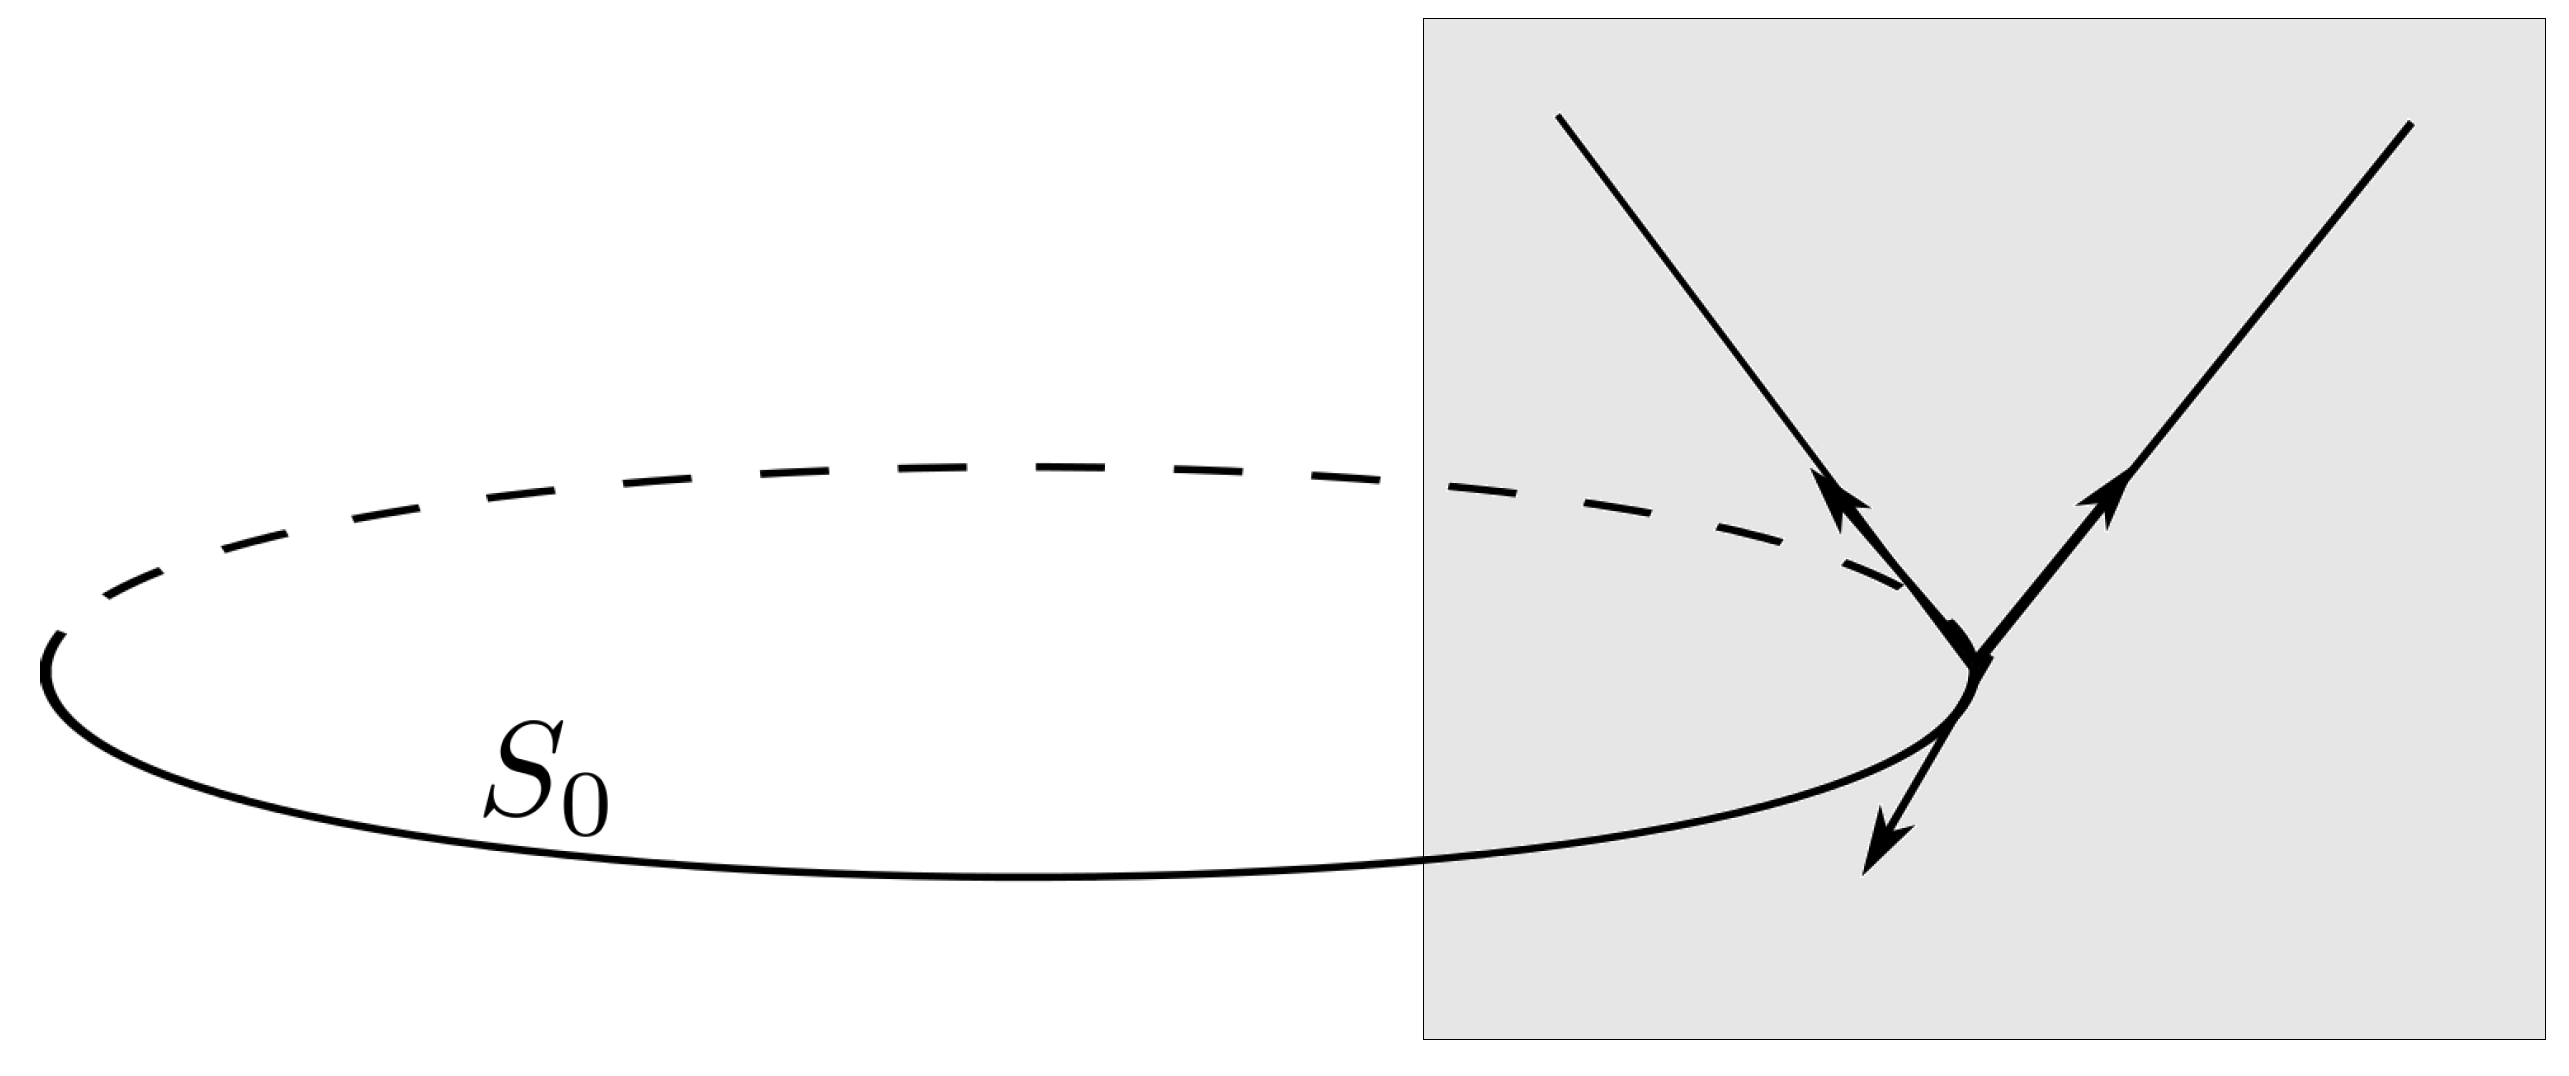
\includegraphics [width=0.75\linewidth] {Pictures/00_Start.png}
\end{center}
Those light directions span 2 surfaces (respectively $C_0$ and $\underline{C}_0$).
\begin{center}
    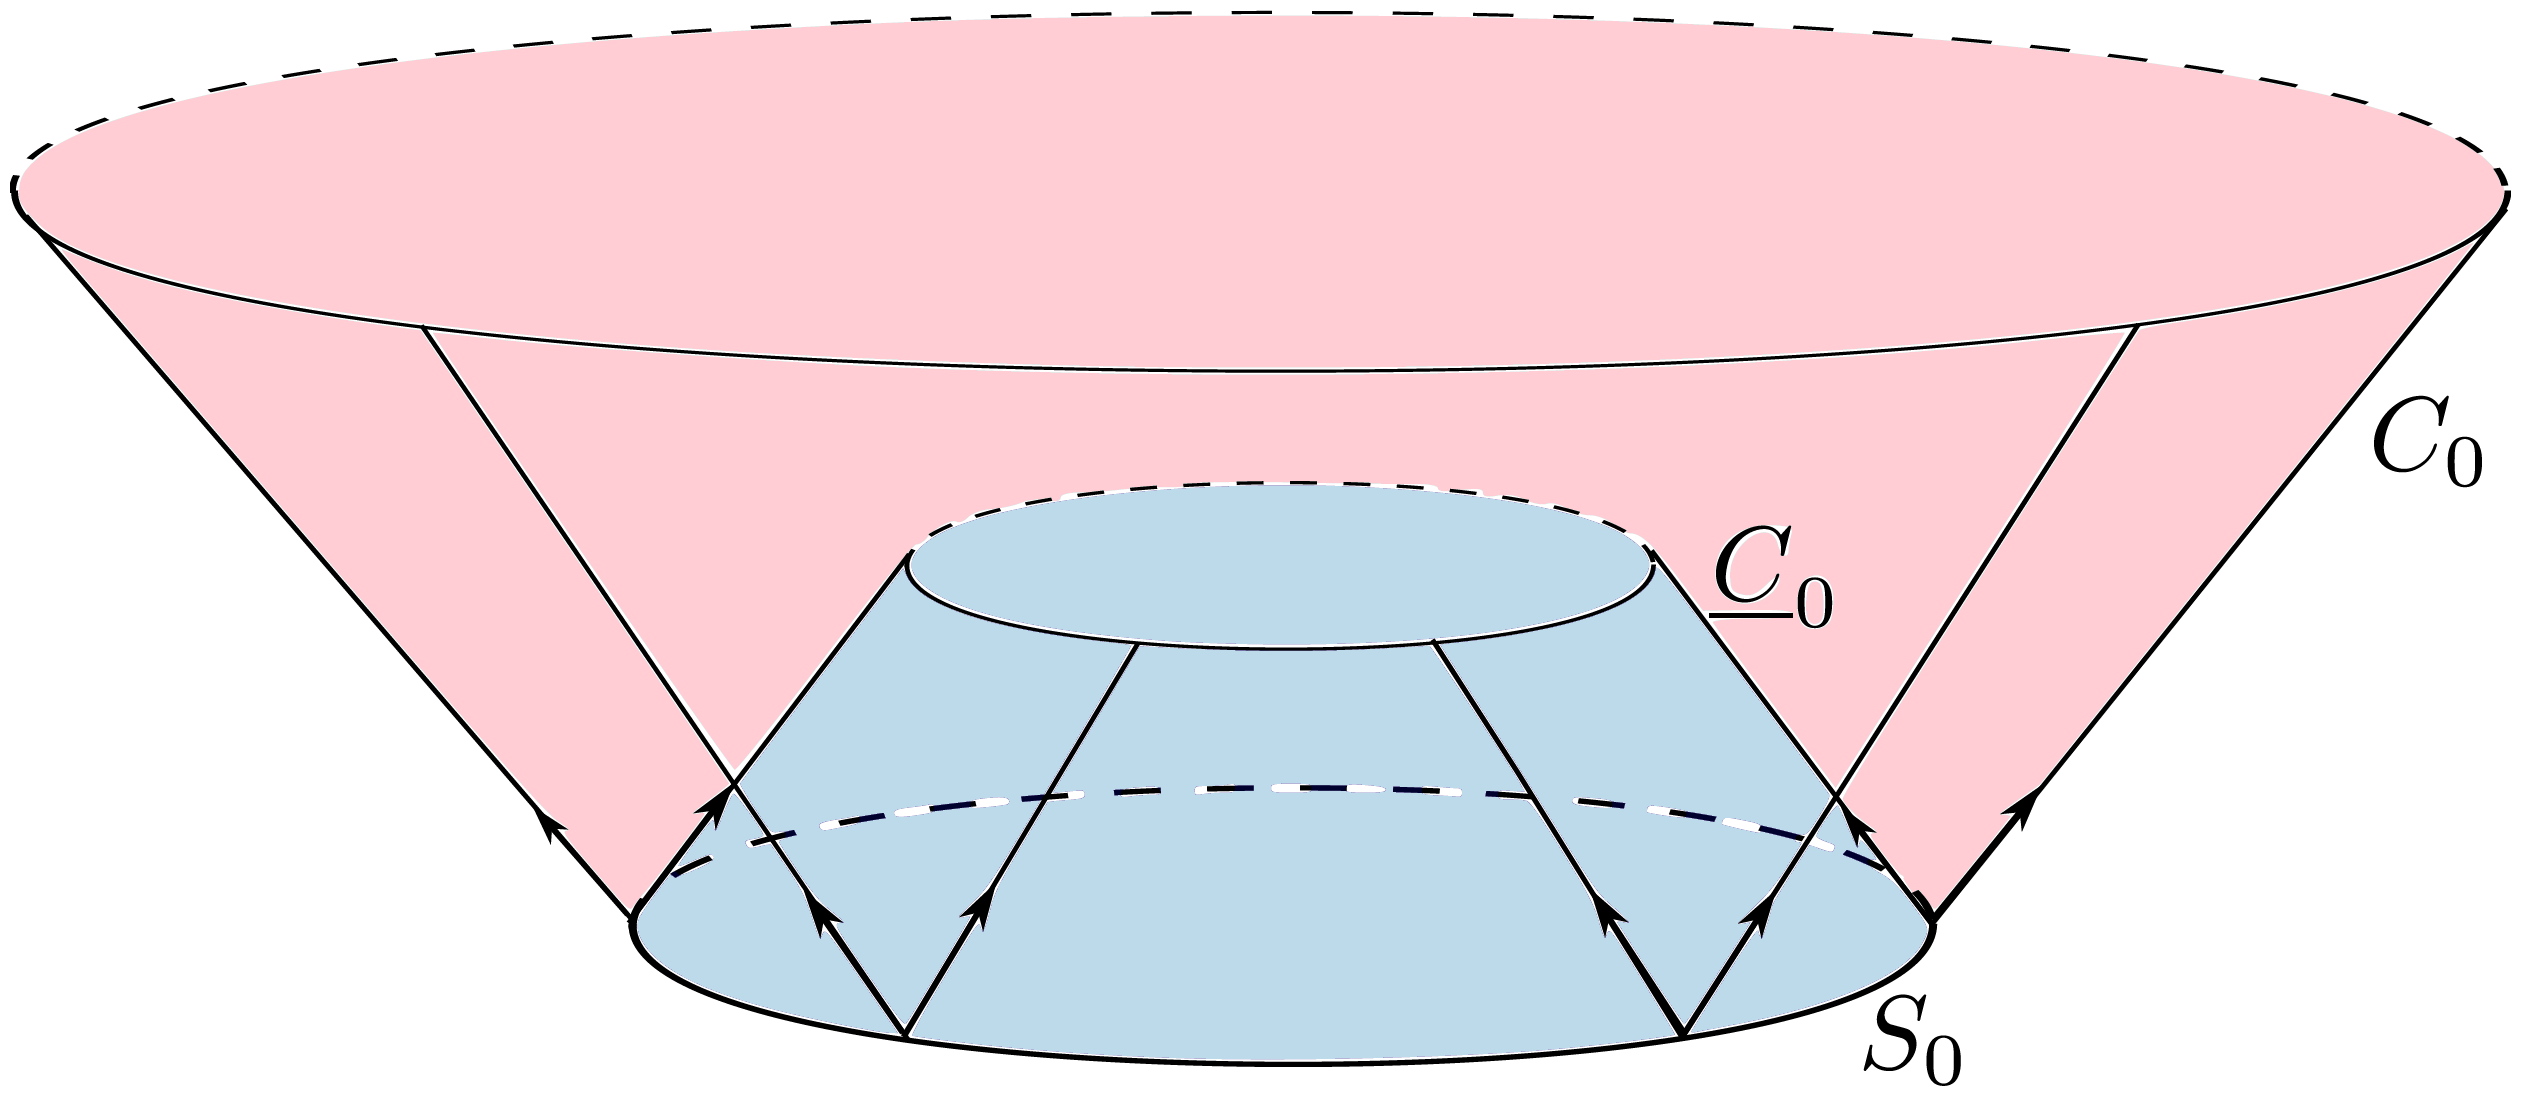
\includegraphics [width=0.75\linewidth] {Pictures/01_Surface.png}
\end{center}

Let $\Omega: S_0 \to \mathbb{R}$ be a smooth function, and $L'$ a null vector field normal to $S_0$ and tangent to $C_0$ (i.e. a continuous choice of one of the null directions at every point). Let $\underline{L}'$ be the null vector field tangent to $\underline{C}_0$ normal to $S_0$ such that $g(L',\underline{L}')=-\Omega^{-2}$ (i.e. the other null direction, but whose norm is constrained by the two other objects).

The steps that follow are going to be many successive extensions of all the previously defined objects.\\
We extend $L'$ and $\underline{L}'$ on $C_0$ and $\underline{C}_0$ through the geodesic equation $\nabla_{L'}L'=0=\nabla_{\underline{L}'}\underline{L}'$ with $\nabla$ the manifold's Levi-Civita connection, with respect to the spacetime metric $g$. Then extend $\Omega$ on $C_0\cup\underline{C}_0$ too. We define $L:=\Omega^2L'$ and $\underline{L} :=\Omega^2 \underline{L}'$ the normalised vector fields.

We now define $\underline{u}$ on $C_0$ to be the vector field such that $L \underline{u}=1$ and $\underline{u}_{|S_0}=0$. (And likewise, $u$ on $\underline{C}_0$.)
\begin{center}
    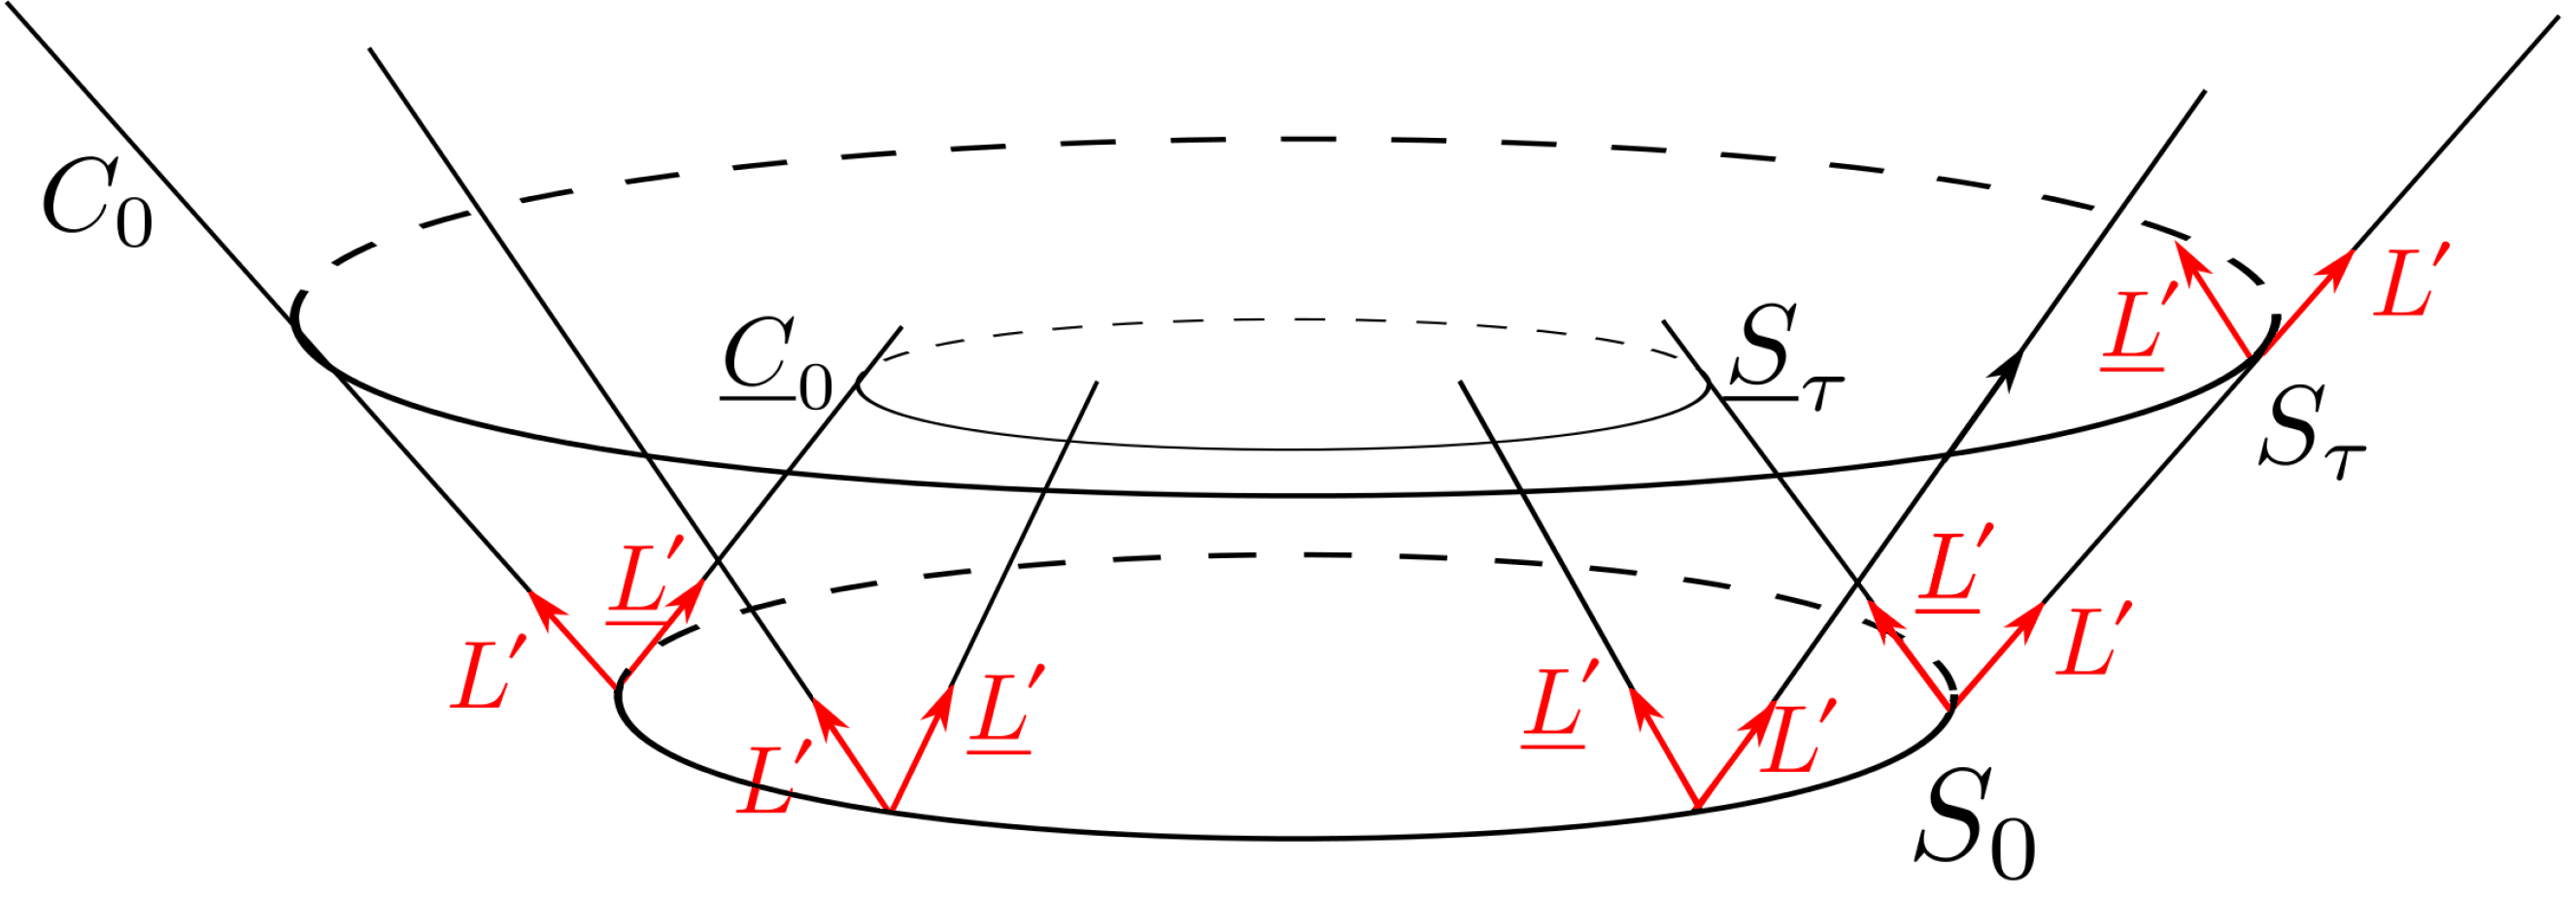
\includegraphics [width=0.75\linewidth] {Pictures/02_VFields.png}
\end{center}

We now notice that there exists\footnote{the differential equations here are all exponential equations, hence the implicit use of bijectivity everywhere here.} $S_\tau$ another embedded co-dimension 2 space-like surface defined by the sets of points on $C_0$ where $\underline{u}=\tau$ (and likewise $\underline{S}_\tau$). $\tau\mapsto S_\tau$ can be seen as a foliation of $C_0$...

We now use these $S_\tau$ as was used $S_0$ to extend the vector field $L$ and $\underline{L}$ on the $C_0$ where they were not yet defined, such that now, all our objects (except for $u$ and $\underline{u}$ at the moment) are defined on $C_0\cup\underline{C}_0$.
\begin{comment}
    Before finishing the construction of the foliation, both \cite{Chris} and \cite{Art} emphasize the fact that $\nabla \underline{u}=-\underline{L}'$ and $\nabla u=-u'$. So we too mention it here, as it probably helps to see $u$ as a potential whose gradient is light-like. This will, of course, also hold on the fully foliated manifold.
\end{comment}

To finish the foliation, we now span, from each $S_\tau$ a $C_\tau$ and a $\underline{C}_\tau$. This concludes the construction of the foliation. Note that this is a \emph{double} foliation, as we have both a foliation in terms of $C_\tau$ and $\underline{C}_\tau$.
\begin{center}
    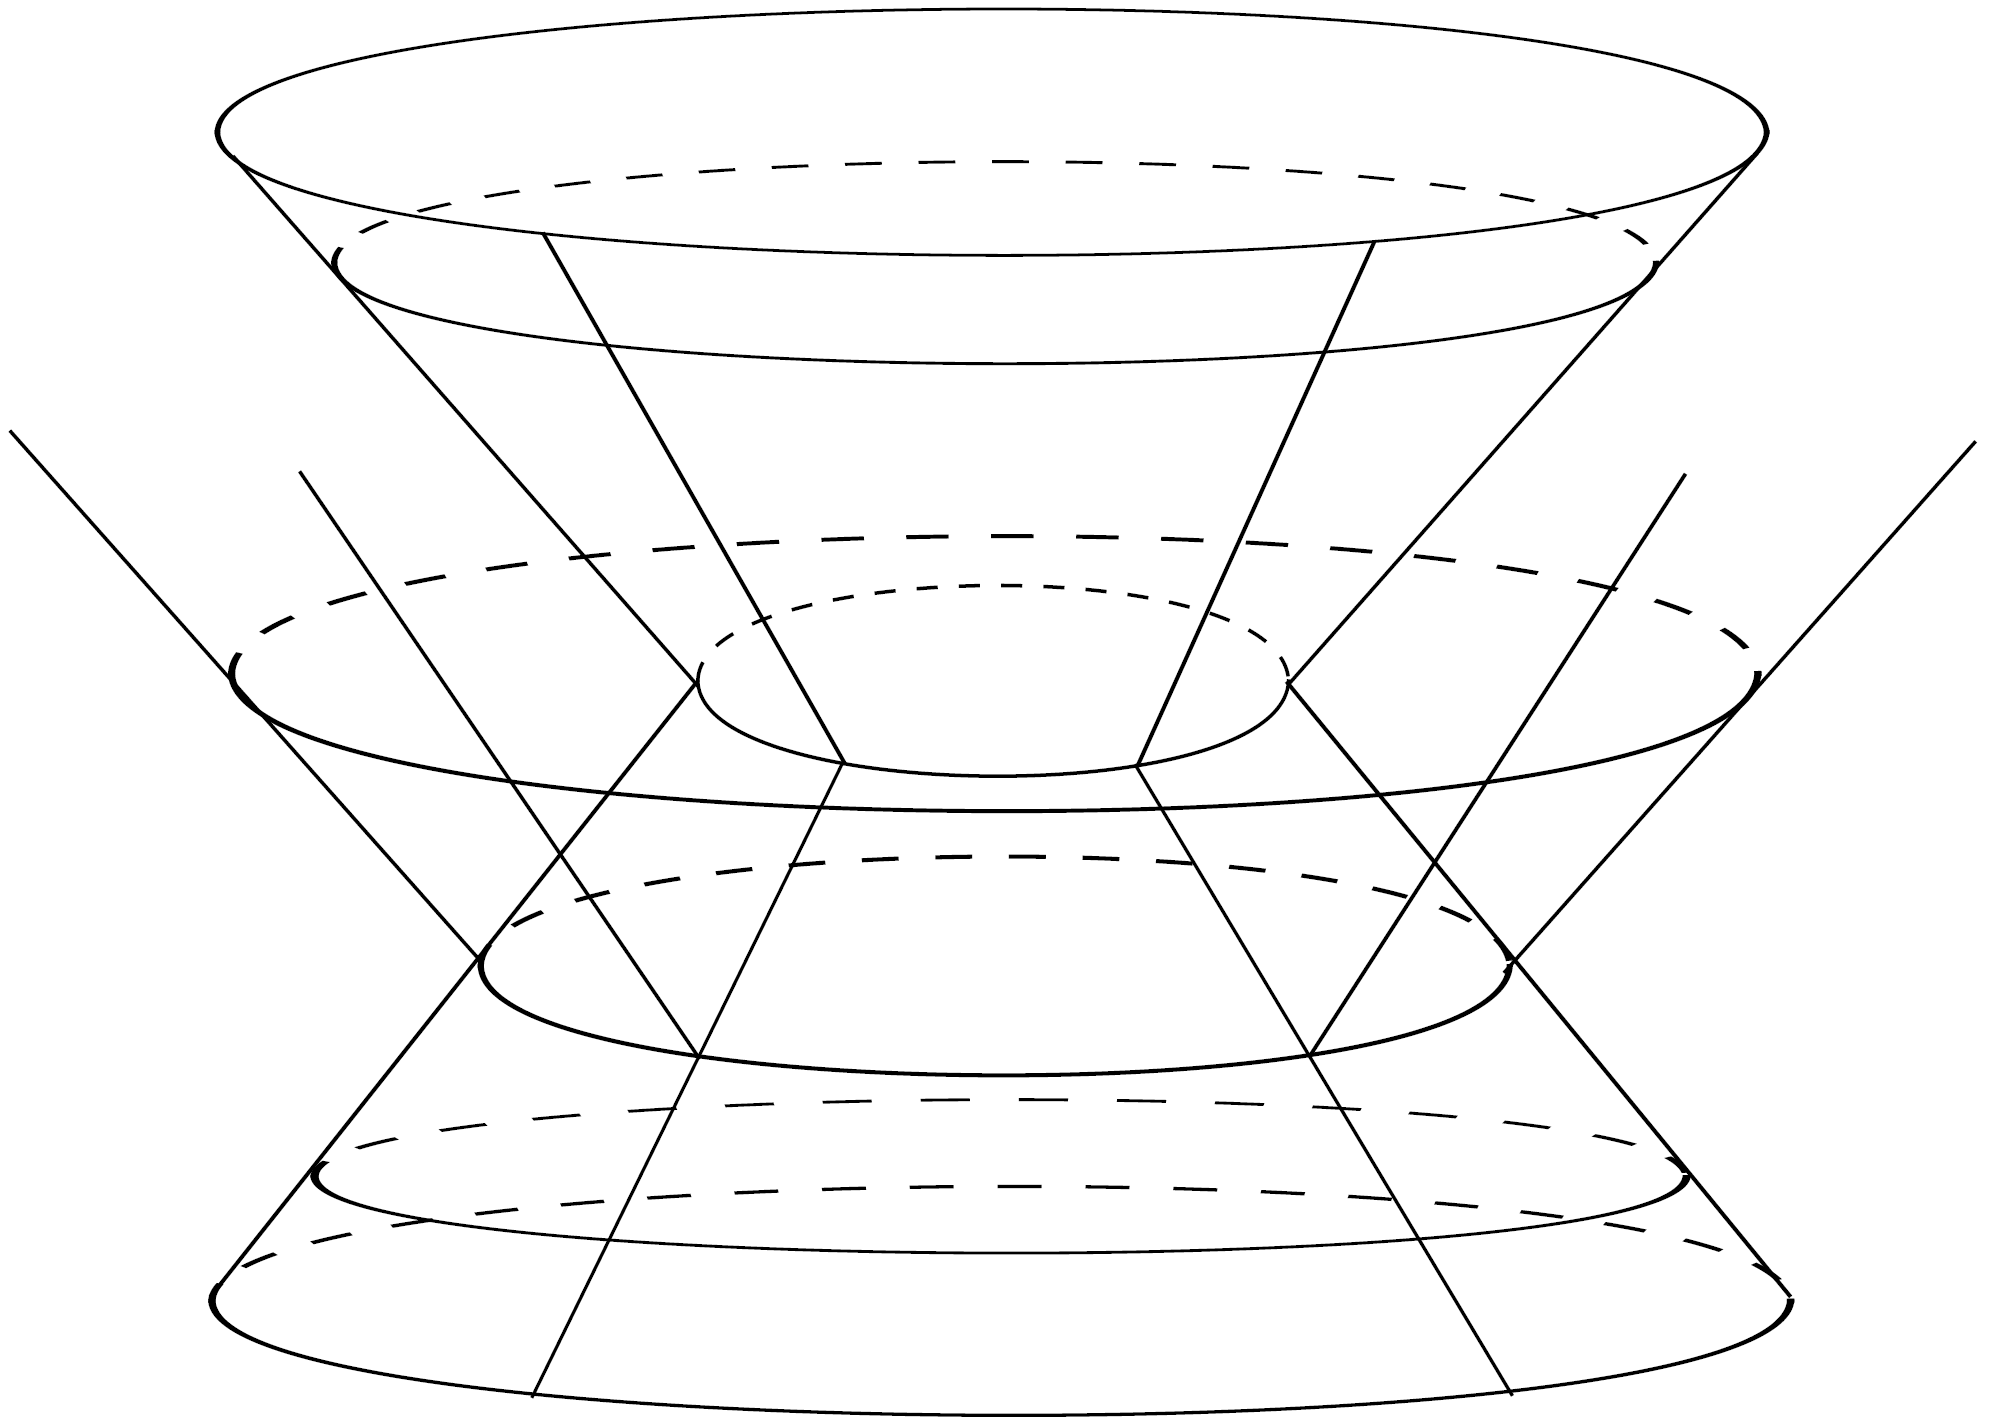
\includegraphics [width=0.75\linewidth] {Pictures/03_Foliation.png}
\end{center}

\subsubsection{Playing around with coordinates}\label{TorsionWarning}
For any point $p$ in thereby foliated spacetime, there exists a null path from $S_0$ to that path. In fact, there even exists a single path starting from a point $\theta^i$ of $S_0$ ($\theta^i$ being given with respect to some coordinate system of the co-dimension 2 manifold $S_0$) then following a the null ray from $\theta^i$ along $C_0$ up to the $\underline{u}$ value of $\underline{u}_0$ and then following the other null direction on $C_{\underline{u}_0}$ until $u_0$. This therefore allows us to have a coordinate system $p=(u_0, \underline{u}_0, \theta^i)$ on the manifold.
\begin{center}
    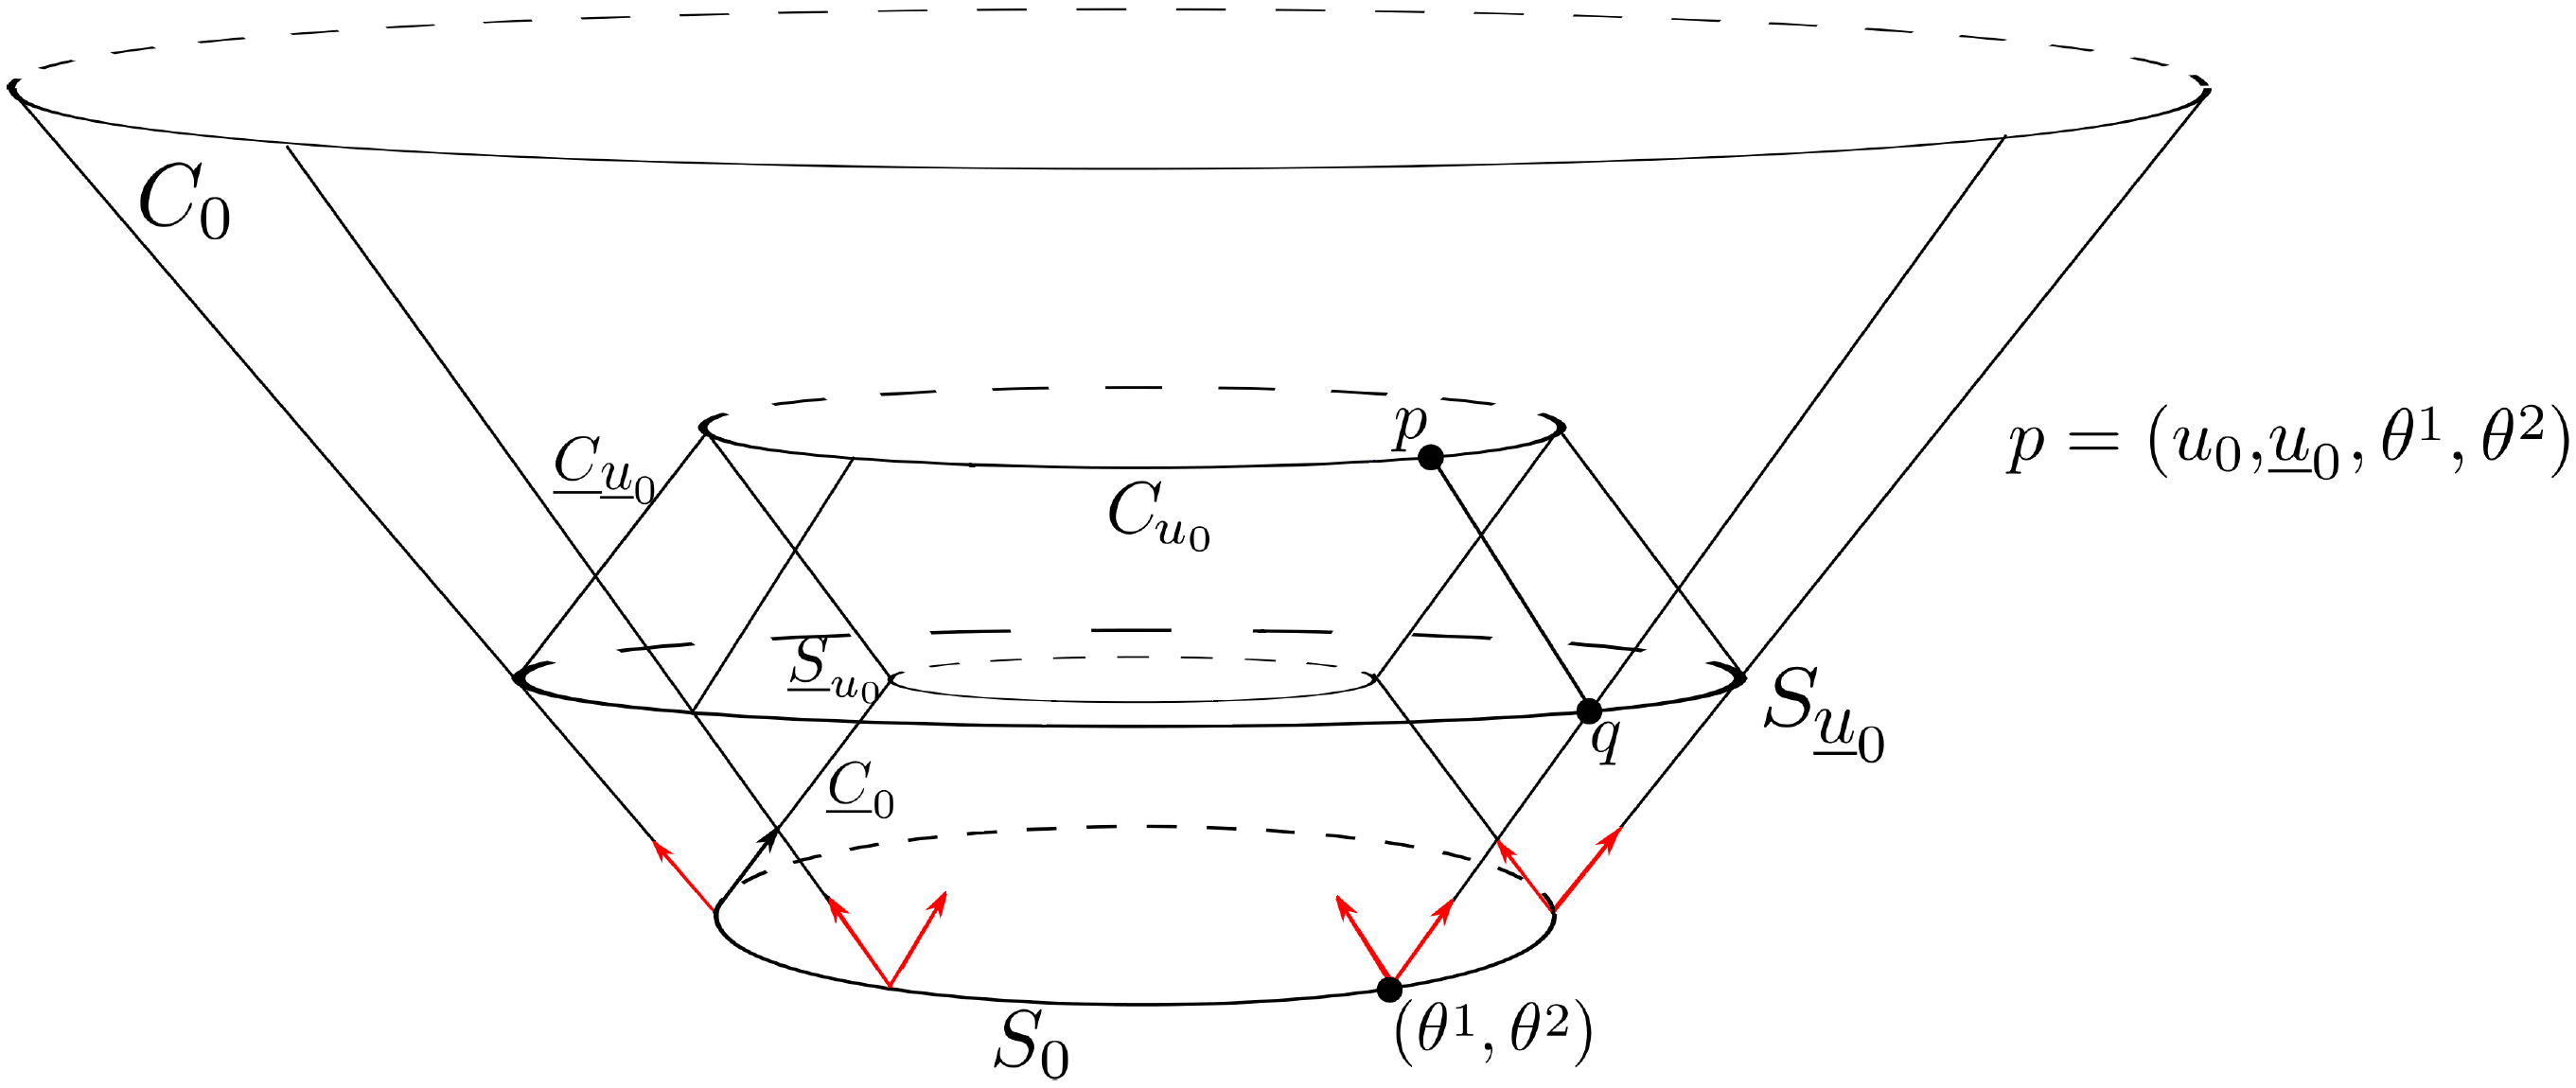
\includegraphics [width=0.75\linewidth] {Pictures/04_Coordinates.png}
\end{center}

Note however that there exists another path by going to $\underline{C}_0$ first and only $C_0$ after, and those two paths do not necessarily share the same values of $u$ and $\underline{u}$... 
\begin{center}
    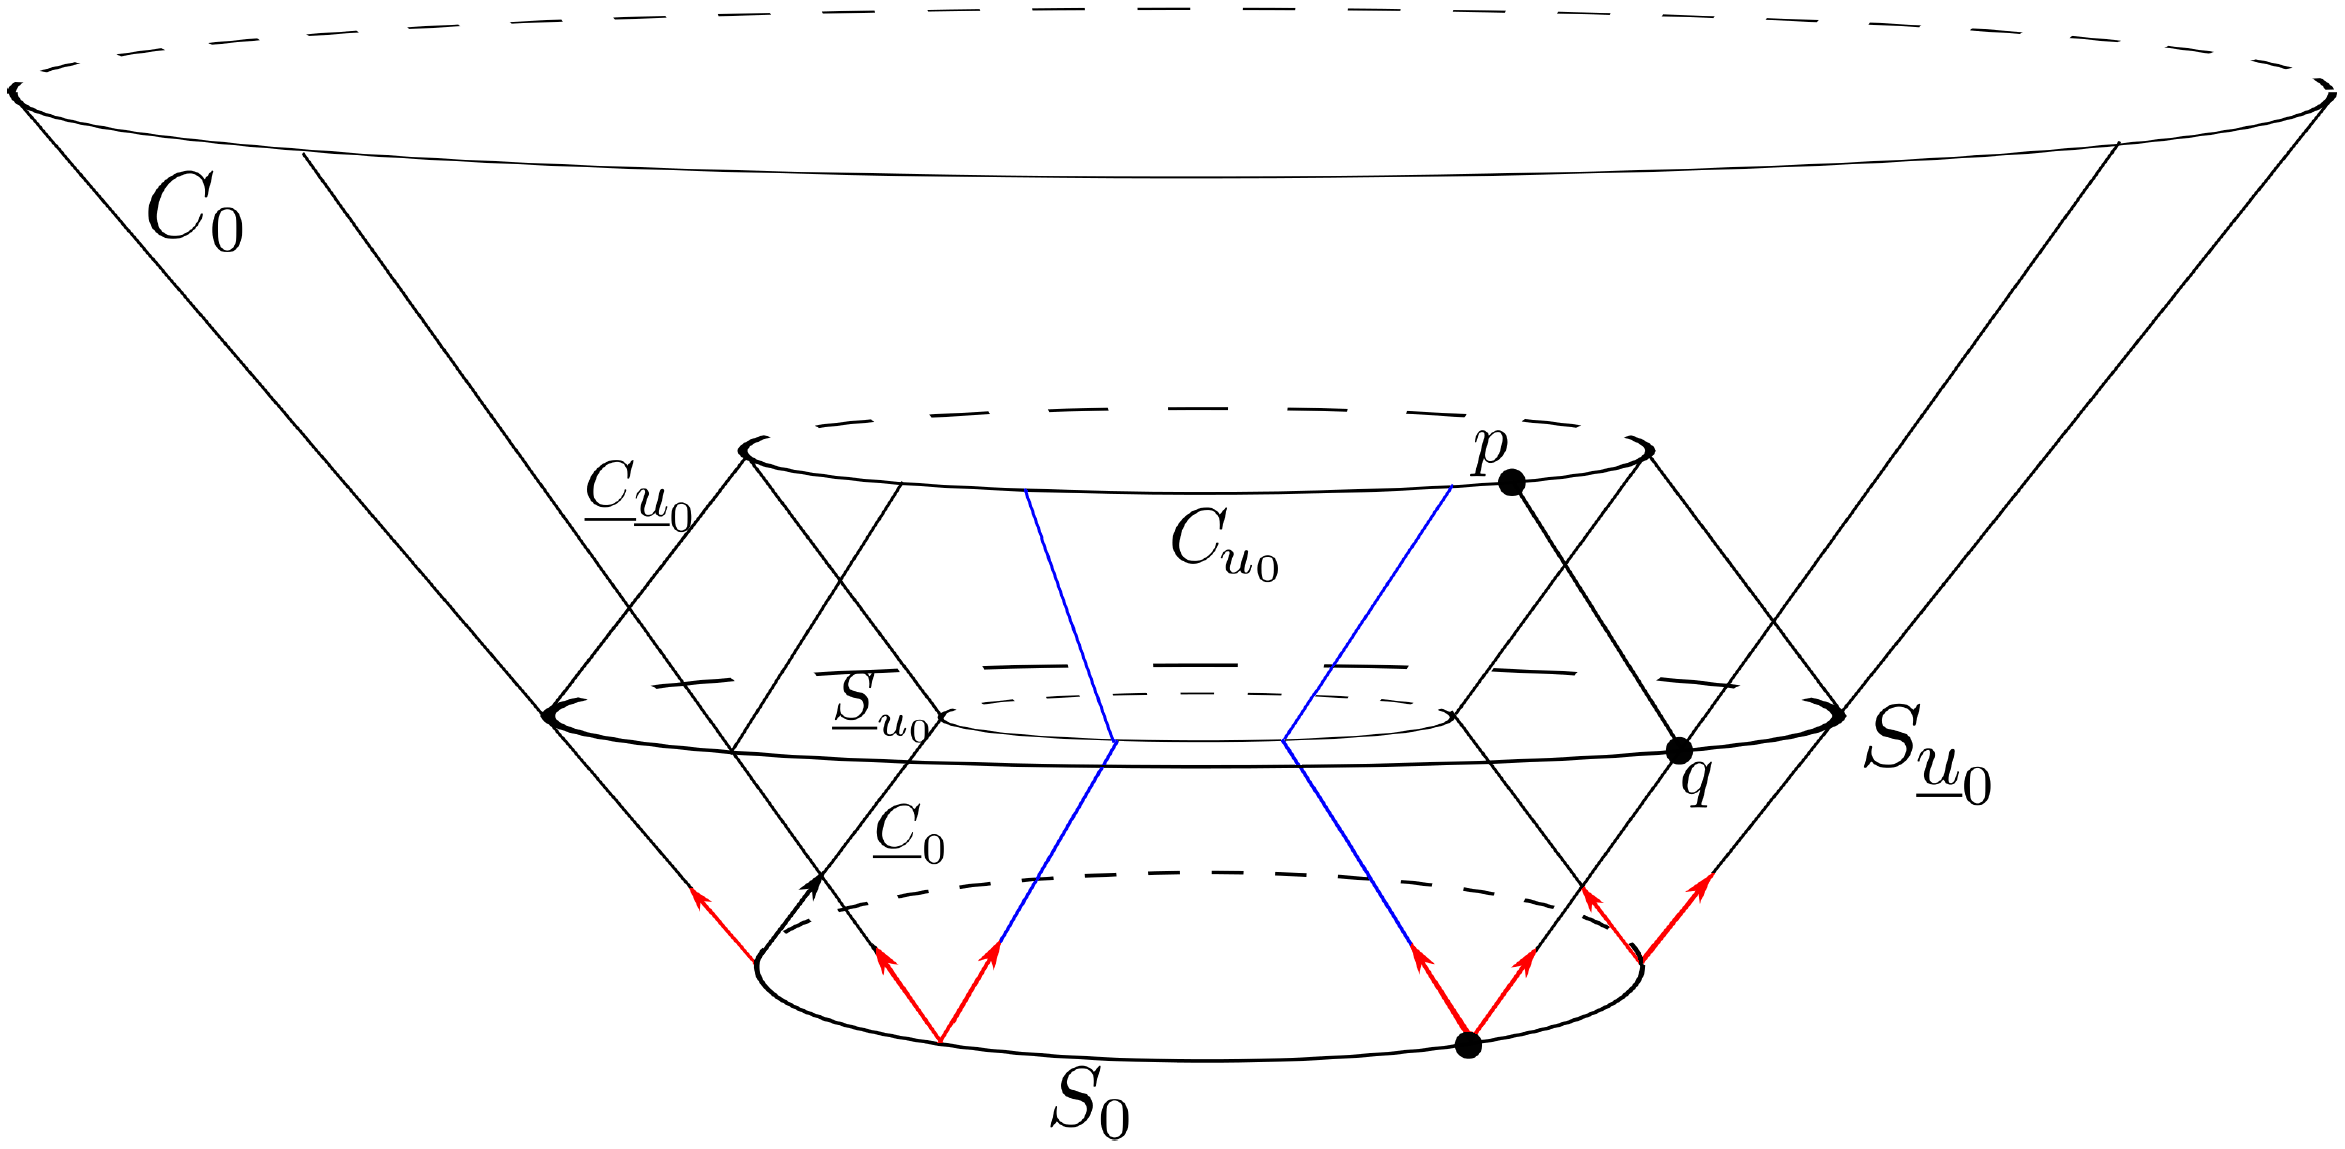
\includegraphics [width=0.75\linewidth] {Pictures/05_Torsion.png}
\end{center}

This is because the two null fields do not commute (in the Lie derivative sense\footnote{Using the vector commutator $[X,Y]:=x^\mu \partial_\mu (y^\nu) e_\nu - y^\mu \partial_\mu (x^\nu) e_\nu = X\circ Y - Y \circ X$ for two vector fields $X:=x^\mu e_\mu$ and $Y:=y^\mu e_\mu$}) unless our metric is somehow trivial. Thus, denoting by $e_i$ the coordinate system of the $C_{u_0}\cap\underline{C}_{\underline{u}_0}$ codimension 2 spacelike manifolds, the tuple $(e_i, L, \underline{L})$ is indeed a \emph{frame} but not a \emph{basis} in true and precise manifold vocabulary.

This does not pose any particularly deep problem when it comes to doing physics in a non-basis frame; but does require a lot of care as many of the formulae familiar to the physicists that are used to derive curvature tensors no longer apply. In particular, $\Gamma_{\mu\nu}^\rho\ne\Gamma_{\nu\mu}^\rho$ and $\Gamma_{\mu\nu}^\rho\ne g^{\rho\lambda}(g_{\lambda\mu,\nu}+g_{\lambda\nu,\mu}+g_{\mu\nu,\lambda})$. So basically, (instead of attempting to re-derive different formulae) we will frequently go back to more formal math notations to ensure clarity.

For our computations, from now on, we chose a normalised frame: $(e_i,e_+,e_-)$ where $(e_i)$ is the coordinate system of the $S$ surfaces, and $e_\pm$ are two null directions normalised to $g(e_+,e_-)=-1$. These can simply be obtained by $e_+:=\Omega\underline{L}'$ and $e_-:=\Omega L'$.

We also inform the reader that in this convention (i.e. the one from \cite{Art}; \cite{Chris}'s only being different by a factor of 2) the metric will be of the following form (where $\cancel{g}$ denotes the metric of the sub-manifold $S$ at any point):
\begin{equation} \label{gNullFoli}
    g=-\d e_+\otimes \d e_- - \d e_-\otimes d\ e_+ + \cancel{g}
\end{equation}
(thus:
\begin{equation}\tag{\ref{gNullFoli}}
g^{-1}=-e_+\otimes e_- - e_-\otimes e_+ + \cancel{g}^{-1} \quad ).
\end{equation}

\begin{comment}[\emph{Difference of notations in mathematics and physics}] \label{NotationWarning}
    In differential geometry, (always using Einstein summation convention of course) there are many types of objects (the zoology of which we will not go into). But it turns out that all of them have (at least) a vector space structure. This leads to every\footnote{We only consider finite dimensional spaces, no need to worry about equivalence classes or choice axiom.} single object being expressible in a basis.
    
    The physicists take great use of this fact and basically only work with the coordinates in a given basis, almost (though not completely I am sure) forgetting the basis itself. This leads physicist to call $x^\mu$ a vector and $g_{\mu\nu}$ an order 2 tensor. This is very practical to them, as it makes explicit computations much easier.

    The mathematicians, on the other hand, tend to have little care about the basis of their spaces, but a lot more about the type of objects they are manipulating. Thus, whenever they use a basis (say $(\partial_\mu)_{\mu \in [\![0,n]\!]}$ or $(\d x^\mu \otimes \d x^\nu)_{(\mu,\nu) \in [\![0,n]\!]^2}$) they really don't lose sight of the difference between coordinates and vectors. Thus, reusing the previous examples, they would call $x^\mu$ an $n$-tuple of scalars, $g_{\mu\nu}$ an $n^2$ one, $x^\mu \partial_\mu$ a vector and $g_{\mu\nu} \d x^\mu \otimes \d x^\nu$ an order 2 tensor.

    Now, so far, this can seem a very pointless difference, not worth so many paragraphs, and to be fair, it almost always it. But it turns out, as our reader will soon see, that we are going to do a lot of explicit computations (thus, will use the physicist's approach) but not in a true vector manifold basis (which will require the mathematician's notation). And although they both look very similar, we will be constantly playing around with the connection, which treats differently objects of different type. Hence, dear reader, we encourage that you keep in mind what is what at all times.
    
    For instance, if $\nabla_\mu$ denotes $\nabla_{e_\mu}$ (i.e. the covariant derivative of the vector $e_\mu$) and $x^\mu e_\mu$ is a vector (with $(e_\mu)$ a basis) then $\nabla_\mu x^\nu=\partial_\mu x^\nu$ and $\nabla_\mu e_\nu = \Gamma_{\mu\nu}^\rho e_\rho$. But if $\nabla_\mu$ denotes the coordinate of the covariant derivative, then $\nabla_\mu x^\mu = \partial_\mu x^\nu +\Gamma_{\mu\lambda}^\nu x^\lambda$ and $\nabla_\mu e_\nu$ is of course an undefined expression.
\end{comment}

\subsubsection{Curvature in null coordinates}
We will now compute the curvature tensor, from the connection. We will straight up reuse the result from \cite{Art} and \cite{Chris} that gives us all non-zero and identical components of the curvature, thus, these are the only things that a courageous reader would have to compute to apply our work to a given metric.

It must be emphasized that we are reusing notations that are very common in the field (identical in every found article using this foliation method) but we will slightly twist it around to fit our personal needs. Indeed, as we (unlike the articles we found) do a lot of explicit computations, we chose a slightly more convoluted notation to make use of the $\pm\mapsto\mp$ symmetry in all equations. If you are comparing with \cite{Art} and \cite{Chris}, apply the following redefinitions:
\begin{align}
    ``+":=3, && ``-":=4, && \underset{+}{\omega}:=\omega, && \underset{+}{\chi}:=\chi, && \underset{+}{\eta}:=\eta.
\end{align}

Note however that we do keep, in all this subsubsection, the mathematician's notation $\nabla_\mu:=\nabla_{e_\mu}$ as do both \cite{Art} and \cite{Chris}, in order to make it easier for the reader to compare our results with them (who do similar computations but with the extra assumption of the metric being a solution to Einstein's vacuum equations). This will mean that $\nabla_\mu e_\nu = \Gamma_{\mu\nu}^\rho e_\rho$ and $\nabla_\mu e_\nu \ne \partial_\mu e_\nu - \Gamma_{\mu\nu}^\rho e_\rho$. We apologies for potentially caused confusion.

Now that those subtleties about notation have been dealt with, let us steal from \cite{Art} and \cite{Chris} the list of all non-zero Christoffel symbols.
\begin{align}
    \underset{\pm}{\chi}\,_{ij} :=&\Gamma_{ij}^\pm, &\Gamma_{i\pm}^j&=\underset{\mp}{\chi}\,_{ik}g^{jk}\notag,\\
    \underset{\pm}{\eta}\,_i :=&\Gamma_{\pm i}^\pm, &\Gamma_{\pm\mp}^i&=\underset{\pm}{\eta}\,_kg^{ik}\notag,\\
    \underset{\pm}{\omega}:=&\Gamma_{\mp\mp}^\mp, &\Gamma_{\mp\pm}^\pm&=-\underset{\pm}{\omega}\label{Christoffel},\\
    \zeta_i :=& \Gamma_{i+}^+ &\Gamma_{i\pm}^\pm&=\pm\zeta_i \notag,\\
    \Gamma_{\pm i}^j&\notag,\\
    \Gamma_{ij}^k&\notag,
\end{align}
where the ones on the left are the only degrees of freedom (so the only ones a courageous reader would have to compute to apply our work to a given spacetime\footnote{The minimal number of calculations to get them all is obtained by only skipping $\nabla_\pm e_\mp$ among all conceivable $\nabla_\mu e_\nu$; which is very disappointing. But if one can compute $\Gamma_{\mu\nu}^\rho$ separately, then the left column is what will be the fastest.}).

Let us now compute commutators $[e_\mu,e_\nu]$ as they will be relevant later on. Although this might seem like something that would need to be computed back at the level of the foliation, we can make use of the fact that (although we do not have $\Gamma_{\mu\nu}^\rho=\Gamma_{\nu\mu}^\rho$) our connection is indeed the levi-cevita connection. It is defined as the (single) connection with no torsion. Since torsion is formally the following tensor:
\begin{equation}
\forall (X,Y) \in T\mathcal{M}^2 \quad\quad  \mathrm{Tor}_\nabla(X,Y):= \nabla_XY-\nabla_YX-[X,Y].
\end{equation}
We can make use of the following equation, as in our case $\mathrm{Tor}_\nabla=0$.
\begin{equation}
    [e_\mu,e_\nu]=\Gamma_{\mu\nu}^\rho e_\rho-\Gamma_{\nu\mu}^\rho e_\rho.
\end{equation}
Our computations yield:
\begin{align}
    [e_\pm,e_\mp]&=\Gamma_{\pm\mp}^\mu e_\mu - \Gamma_{\mp\pm}^\mu e_\mu\notag\\
    &=\Gamma_{\pm\mp}^i e_i - \Gamma_{\mp\pm}^i e_i + \Gamma_{\pm\mp}^\pm e_\pm - \Gamma_{\mp\pm}^\pm e_\pm + \Gamma_{\pm\mp}^\mp e_\mp - \Gamma_{\mp\pm}^\mp e_\mp\notag\\
    &=\underset{\pm}{\eta}\,_jg^{ij} e_i - \underset{\mp}{\eta}\,_jg^{ij} e_i + 0 + \underset{\pm}{\omega} e_\pm - \underset{\mp}{\omega} e_\mp - 0\notag\\
    &=(\underset{\pm}{\eta}-\underset{\mp}{\eta})\,_jg^{ij} e_i+ \underset{\pm}{\omega} e_\pm - \underset{\mp}{\omega} e_\mp\label{[pm,mp]};
\end{align}
\begin{align}
    [e_\pm,e_i]&=\Gamma_{\pm i}^\mu e_\mu - \Gamma_{i\pm}^\mu e_\mu\notag\\
    &=\Gamma_{\pm i}^k e_k - \Gamma_{i\pm}^k e_k + \Gamma_{\pm i}^\pm e_\pm - \Gamma_{i\pm}^\pm e_\pm + \Gamma_{\pm i}^\mp e_\mp - \Gamma_{i\pm}^\mp e_\mp\notag\\
    &=\Gamma_{\pm i}^k e_k - \underset{\mp}{\chi}\,_{ij}g^{jk} e_k + \underset{\pm}{\eta}\,_i e_\pm \mp \zeta_i e_\pm + 0 - 0\notag\\
    &=(\Gamma_{\pm i}^k - \underset{\mp}{\chi}\,_{ij}g^{jk}) e_k + (\underset{\pm}{\eta}\,_i \mp \zeta_i) e_\pm \label{[pm,i]};
\end{align}
and of course, since the $e_i$ vectors are proper space-like basis or the submanifold $S_{u\underline{u}}$, 
\begin{equation}[e_i,e_j]=0 \label{[i,j]}.\end{equation}
We can now attempt computing the Rieman tensor. As for the Christoffels, since we are not in a proper coordinate system, we must go back to the original formula:
\begin{equation}
    \forall (X,Y,Z)\in T\mathcal{M}^3 \quad \quad \mathrm{Riem}_\nabla (X,Y)Z:= \nabla_X\nabla_YZ-\nabla_Y\nabla_XZ-\nabla_{[X,Y]}Z.
\end{equation}
Which we can, in turn, express in our frame (using the image of it) into:
\begin{equation}
\mathrm{Riem}_\nabla (e_\mu,e_\nu)e_\sigma =: R^\rho_{\;\sigma\mu\nu} e_\rho.
\end{equation}
Which gives us an expression (but is not as satisfying as in the coordinate case):
\begin{equation}\label{Riem_munu}
    R^\rho_{\;\sigma\mu\nu} e_\rho = \nabla_\mu\nabla_\nu e_\rho-\nabla_\nu\nabla_\mu e_\rho-\nabla_{[e_\mu,e_\nu]}e_\rho.
\end{equation}
We notice that the famous property $R^\rho_{\;\sigma\mu\nu}=-R^\rho_{\;\sigma\nu\mu}$ trivially holds.\\
Other symmetries of the tensor require the lowering of $\rho$, so we will simply not use them. We do not detail here the derivation of the $R^\rho_{\;\sigma\mu\nu}$ as it is long, tedious, and frankly uninteresting. But one can find the detailed steps in the appendix on page \pageref{CompR}.
\subsection{Computation of the Inequality and future use}
\subsubsection{Computing $C$}
Recall our current state of the computation of our inequality:
\begin{equation}\tag{\ref{eq82}}
    \boxed{\int_\Sigma \!\!\!\d_\mathrm{vol} g^2 \!\braket{l^\mu l^\nu T^\mathrm{ren}_{\mu\nu}}_{\!\psi} \!\!\geq\!\!\! \int_\Sigma \!\!\!\d_\mathrm{vol} g^2l^\mu l^\nu C_{\!\mu\nu}\!-\!2\!\!\!\int_D\!\!\frac{\d^n\xi}{(2\pi)^n}\!\left(\!\!(|h_\kappa|^{\!^1\!\!/_{\!4}}\!g_\kappa\!)^{\!\otimes 2}\vartheta_\kappa(l^\mu\nabla_\mu\!\otimes l^{\nu'}\nabla_{\nu'}\mathcal{FT}_{\!\!H_{(2)}}\!\!\right)^{(-\xi,\xi)}}\;.\!\!\!
\end{equation}
We will focus on the term $C_{\mu\nu}$'s computation. We mentioned previously (on page \pageref{T_ren}) that :
\begin{equation}\tag{\ref{T_ren}}
    \braket{T^\mathrm{ren}_{\mu\nu}}:=\braket{T^\mathrm{fin}_{\mu\nu}}-Qg_{\mu\nu} + C_{\mu\nu}.
    \end{equation}
Let us be more precise. In \cite{QFTCurv}, we find that the coefficient is:
\begin{equation}
    -Qg_{\mu\nu}+C_{\mu\nu}=\alpha^{(1)}\mathcal{H}_{\mu\nu}+\beta^{(2)}\mathcal{H}_{\mu\nu}+\gamma\mathcal{H}_{\mu\nu},
\end{equation}
where:
\begin{align}
    ^{(1)}\mathcal{H}_{\mu\nu}:=& 2R_{;\mu;\nu}+ 2g_{\mu\nu}\square R - \frac{1}{2}g_{\mu\nu} R^2 + 2 R\cdot R_{\mu\nu}\notag;\\
    ^{(2)}\mathcal{H}_{\mu\nu}:=& R_{;\mu;\nu} - \frac{1}{2}g_{\mu\nu}R-\square R_{\mu\nu} -\frac{1}{2} R^{\alpha\beta}R_{\alpha\beta}+2R^{\alpha\beta}R_{\alpha\beta\mu\nu};\\
    \mathcal{H}_{\mu\nu}:=& 2R_{\mu\alpha\beta\gamma}R_\nu^{\;\alpha\beta\gamma}-4\square R_{\mu\nu} -\frac{1}{2}g_{\mu\nu}R^{\alpha\beta\gamma\delta}R_{\alpha\beta\gamma\delta} + 2 R_{;\mu;\nu} - 4 R_{\mu\alpha}R^{\alpha}_{\;\nu}+4R^{\alpha\beta}R_{\alpha\mu\beta\nu}\notag.
\end{align}
This yields:
\begin{align}
    C_{\mu\nu} &= 2\alpha R_{;\mu;\nu} + \beta R_{;\mu;\nu} - \beta\square R_{\mu\nu} +4\gamma \square R_{\mu\nu} + 2\gamma R_{;\mu;\nu} + \mathcal{O}(R^2)\notag\\
    &= (2\alpha + \beta + 2\gamma) R_{;\mu;\nu} +(4\gamma- \beta)\square R_{\mu\nu} + \mathcal{O}(R^2) \label{C=A+B}.
\end{align}

But as we saw in section \ref{TorsionWarning} (page \pageref{TorsionWarning}), we need to remember that these expressions hold for coordinates in a \emph{basis}, whereas we wish to express them in our non-basis frame. To know exactly how this will end up looking, we will simply express the tensor $C$ without any reference to the basis $e_\mu$ and then, get its coefficients in the frame $(e_i,e_+,e_-)$.

Note that in this section, we will use the notation of $\nabla_\mu$ of the physicist, i.e. that of the coordinates. Thus $\nabla_\mu \ne \nabla_{e_\mu}$. This is because \cite{QFTCurv} uses this one, so when we write $R_{;\mu;\nu}$ it means $\nabla_\mu \nabla_\nu R$ only in the physicist sense, and likewise for $\square:=\nabla_\rho \nabla^\rho$ in the physicist's way. We apologies for potentially caused confusion. Feel free to refer to comment \ref{NotationWarning} (on page \pageref{NotationWarning}) for more details.

Now, the here-above expression of $C_{\mu\nu}$ is in a proper basis, one where the coordinate fields commute. So, to be sure that we do not make any mistakes when changing to our non-commutative frame, we will compute the mathematical tensor:
\begin{equation}
C : \Bigg\{\begin{matrix}
    T\mathcal{M}^{\otimes2} & \to & \mathbb{R}\\
    (x^\mu e_\mu, y^\nu e_\nu) & \mapsto & x^\mu y^\nu C_{\mu\nu}
\end{matrix}
\end{equation}
in a form that doesn't use any coordinate representation, then we will be able to evaluate it back in our frame, without any worries of what having non-commutative coordinate fields could cause being slightly different.

Then, we choose $l^\mu \partial_\mu$ to be along one of our null foliation coordinate $e_\pm$. \\
Leading to $l^\mu \partial_\mu = x_\pm e_\pm$ and the following integral:
\begin{equation}
    \int_\Sigma \d_\mathrm{vol}g^2 l^\mu l^\nu C_{\mu\nu} = \int_{\mathbb{R}\times \mathbb{R}\times S} \!\!\!\!\!\!\!\!\!\!\!\!\!\!\! \d_\mathrm{vol} \cancel{g}^2 \d x_\mp \d x_\mp' \d x_\pm \d x_\pm ' \;\cdot \; x_\pm x_\pm ' C_{\pm\pm}(x_i,x_\pm, x_\mp)\; ,
\end{equation}
with $C_{\pm\pm}:= C(e_\pm,e_\pm)$ of course. Proof of the measure's decomposition $\d_\mathrm{vol}g = \d x_\pm \d x_\mp \d_\mathrm{vol} \cancel{g}$ can be found in \cite{Art}. This also implies that $l^\mu \nabla_\mu$ will be $x_\pm \partial\pm$ when applied on to $\mathcal{FT}_{H_{(2)}}$.

Now this computation is quite lengthy, and although the part where we get $C$ is interesting, computing $C_{\pm\pm}$ is painfully long and interesting. So we do not write it here, but we let the interested reader find it in the commutation appendix. (Moreover, as we shall see later, we do not need its expression, but rather only a lower bound for it.)


\subsubsection{Computing $H$}
In this section, each time we quote a formula, unless it is one we already saw before, it comes from \cite{HadRen}, where all computational details about Hadamard states can be found.

We sadly didn't get to compute the $H$ part of the inequality in time. So this part is more of a guideline of what we will attempt to do next, in order to compute things. Computation steps are reasonably easy to understand, but like in the case of $C_{\pm\pm}$ or the curvature, the actual expressions get lengthy quite fast, which is why, in practice, it is easier said than done.

We recall from section \ref{DefHad} that the Hadamard parametric (i.e. the two point function, but made real), and thus its 3 components $U$, $V$, and $W$,  can be tailor expanded in the geodesic distance $\sigma$. Then, making that parametric on shell (i.e. imposing the equations of motions) we get the following equations:\\
$\forall n \in \mathbb{N}^*$
\begin{equation}
    (2n+2-D) \left( n - \Delta^{-^1\!/_2} \Delta^{\!^1\!/_2}_{\;\;\; ;\mu} \sigma^{;\mu} + \sigma^{;\mu}\partial_\mu \right) U_n + \left(\Box_x -m^2 - \xi R\right) U_{n-1} = 0;
\end{equation}
\begin{equation}
    U_0=\Delta^{\!^1\!/_2};
\end{equation}
\begin{equation}
    n \left(D + 2 \sigma^{;\mu}\partial_\mu -  2 \Delta^{-^1\!/_2} \Delta^{\!^1\!/_2}_{\;\;\; ;\mu} \sigma^{;\mu}\right) V_n + \left( \Box_x - m^2 - \xi R\right)=0;
\end{equation}
\begin{equation}
    \left( D-2 + 2 \sigma^{;\mu} \partial_\mu - 2 \Delta^{-^1\!/_2} \Delta^{\!^1\!/_2}_{\;\;\; ;\mu}\sigma^{;\mu} \right) + \left( \Box_x - m^2 - \xi R\right) U_{D/2 - 2} = 0;
\end{equation}
\begin{align}
     n \Big(2n -2 + D + 2 \sigma^{;\mu} \partial_\mu - 2 \Delta^{-^1\!/_2} \Delta^{\!^1\!/_2}_{\;\;\; ;\mu}\sigma^{;\mu}\Big) \;&\; W_n\notag\\
+ \Big((4 n -2 + D) + 2 \sigma^{;\mu} \partial_\mu - 2 \Delta^{-^1\!/_2} \Delta^{\!^1\!/_2}_{\;\;\; ;\mu}\sigma^{;\mu} \Big) \;&\; V_n \\ + \left( \Box_x -m^2 - \xi R\right) \;&\; W_{n-1} = 0 \notag ;
\end{align}
where:
\begin{equation}
    \boxed{\Delta(x,x') := - \big(\mathrm{det}|g|\big)^{-^1\!/\!_2}(x) \mathrm{det}|\sigma_{;\mu ;\nu'}|(x,x')\big(\mathrm{det}|g|\big)^{-^1\!/\!_2}(x')}\;.
\end{equation}
Now, two things need to be noticed.

The first one is that, all indices-related objects are either of the form $f_{;\mu}$ where $f$ is a scalar field; or $\Box_x f$ where $f$ is also a scalar field. So in the first case, no need to involve our complicated connection, everything works our fine, and for the box, it's a bit more non-trivial, but works like for the computation of the $A_{\pm\pm}$ coefficient in the computation of $C_{\pm\pm}$ so nothing we cannot handle in our frame.

The second is that we do not need to compute all the $(U_n, V_n, W_n)$ terms, \color{red} as we only go up to $H_{(k)}$\color{black}. So we will just try to express everything using minimal amount of terms (to basically get everything in terms of ``initial conditions", i.e. properties of the states as local as can be).

The result of that computation of \color{red}$H_{(k)}$\color{black} will be a scalar field itself. So the integral, the $l^\mu \nabla_\mu$ will simply give us an $x_\pm \partial_\pm$.
As for the Fourier transform's computation, there is no problems with it, we need not worry about any curved space aspect, as $D\subset \mathbb{R}^n$ and, the power of distributions is that we can also ignore $D\ne \mathbb{R}$ by restricting the support of the test function and integrating over all $\mathbb{R}^n$.

So, overall, although those are long and painful computations and we had too little time to perform them ourselves, there is no intrinsic difficulty in them. For an example of those calculations in a different case (time-like inequality) see \cite{TimeLikeCompute}.
\subsubsection{Use}
We will now impose a bound on the curvature. That is (in our frame):
\begin{align}
    |R_{\mu\nu}| &\leq R_\mathrm{max}&
    |\partial_\rho R_{\mu\nu}| &\leq
    R_\mathrm{max}'&
    |\partial_\rho\partial_\sigma
    R_{\mu\nu}| & \leq R_\mathrm{max}''&
    \mathrm{ect}...
\end{align}
We know these bounds to be in $\mathcal{O}(R)$ and we only work at first order in $R$.

From these bound one can \color{red} although I have not managed to, yet \color{black} extract a bound on every single component of the connection. This allows, in turn, to confine $C_{\pm\pm}$ only with these bounds and $\alpha$, $\beta$ and $\gamma$, the renormalisation freedom. It also allows to confine and $\Delta$ only with the curvature bounds and from that, to also confine the $H$ part of the inequality in terms of those curvature bounds and the specificity of the state. \color{red} Provided I can get rid of the metric coefficients too. \color{black}

Now, we must (if we are to begin computations) make $D$ explicit in some way. We must be careful, for most choices of $D$ brake covariance. Thus, it is more likely we will try to look for a set $D$ that, altogether, ensure covariance, and then manually optimize the resulting bound; in the spirit of what was done in the flat case, in section \ref{FlatCase}, using boosts to have covariance and optimizing on them.

Once all this is explicitly written and computed, we are left with a lower bound on the QFT's energy density exclusively dependent on the curvature's extrema and the specificities of a given state. It is from that very bound that the making of singularity theorems can be started.

Although we do not go into the realm of singularity theorems in the present work, we can roughly explain the intuition from here: one can assume a particular topology or causal structure, integrate the inequality along it following Einstein's equations of motion, and get a contradiction; thereby formally excluding some spacetimes.

\section{Conclusion}
\color{red}
Also add choice of D in the future use;
Bound $C_\pm\pm$;
Formula by wiser (47 in her time-like paper)\color{black}

Although time was too short to compute explicitly the Double Smeared Null Energy Condition, i.e. to express it purely in terms of known algebraic functions and lower bounds on the curvature and its derivatives, we have done a significant part of the work. It remains to \color{red} ??? \color{black} and then the inequality with be ready for future use.

As we mentioned before such an inequality will certainly have applications in finding a singularity theorem associated to the corresponding QFT. This will contribute to the general knowledge of the effect of Quantum Field Theories on a curved spacetime following the General Relativity equations.
\newpage
\appendix
\section{Physics Appendix}
    \subsection{Category, functor, natural transformation} \label{AnPhCat}
    For proper definition, see the math appendix or \cite{AlgLang}.
        \subsubsection{Category}
    Category theory is the study of structures. Formally, a category is a collection of objects and the links between them (links which we call the \emph{morphisms} of the category).\\
    Examples of famous categories are:
    \begin{itemize}
        \item Groups (known in physics as "symmetries"), whose morphisms are group-preserving functions (i.e. $f(a\cdot b)=f(a) \cdot f(b)$)
        \item *Algebras (known in physics as "observables"), whose morphisms are *Algebras preserving functions (i.e. $f(\lambda.a.b+c)=\lambda.f(a).f(b)+f(c)$ and $f(a^\dag)=f(a)^\dag$)
        \item Given a spacetime, the collection of all the charts on it forms a category whose morphism are all the switch to other nearby charts
        \item The category of Feynman diagrams where the morphism are relations between them (like a diagram being a sub-diagram of the other in the non-1PI case, or the replacement of a particular vertex with a different one).
    \end{itemize}
    The power of category-formulated statements is that they are not mathematical objects per say, but are \emph{about} mathematical objects, so they allow to take a useful step back.
    
    In category theory, one usually draws relations in diagrams as follows, and calls them \emph{commutative} whenever all paths are the same. For example, the following diagram defines the multiplication in a $\mathbb{K}$-algebra $A$ (with $\mu$ the algebra product, $\eta$ is the unit element of the algebra).\\
    \begin{tikzcd}
    & \arrow[ld, "\mu\otimes\mathrm{id}"] A\otimes A \otimes A  \arrow[rd, "\mathrm{id}\otimes\mu"]\\
    A\otimes A \arrow[rd, "\mu"]& &\arrow[ld, "\mu"]A\otimes A& & A \otimes A \arrow[rd, "\mu"]& & A\otimes A \arrow[rd, "\mu"]\\
    & A & & & \mathbb{K}\otimes A \arrow[u, "\eta\otimes\mathrm{id}"] \arrow[equal]{r}& A & \arrow[u, "\mathrm{id}\otimes\eta"] A\otimes\mathbb{K} \arrow[equal]{r} & A
\end{tikzcd}
    

    \subsubsection{Functors}
    A functor is an object that sends a category to another cathegory. They are the most important tool in category theory, as they allow formal study of the interaction between two apparently different structures.\\
    Here are examples of famous functors from physics.
    \begin{itemize}
        \item The functor from Lie Groups to Lie Algebras (it sends groups to their tangent planes, and group morphisms into lie Algebra morphisms)
        \item  The "exponential functor", which sends any Lie Algebra to the associated compact Lie Group (it is the \emph{dual} functor to the previous).
        \item The Legendre functor which sends the Euler-Lagrange Picture of Classical Dynamics to the Hamilton-Jacobi Picture
        \item The Fourier Functor which sends Classical Quantum Mechanics from the Position Representation to the Momentum Representation
        \item The Feynman rules functor that sends the category of Feynman diagrams to their values and the relations between them into formulas.
    \end{itemize}
    Having a functor simply means being able to bring some of the interesting things of a structure into another. In our case, (QFT in curved spaces) a functor that we will see all the time is the Algebra Functor, which to any neighbourhood of a spacetime associates all the observables accessible to an observer in that region, and therefore, we see that it is core in the \emph{covariance} requirement of QFT.

    \subsubsection{Natural Transformations}
    We do not use them much in this project but they are still quite important. A natural transformation is a \emph{morphism between functors} from a category to another. They allow to study functors themselves as a category (and thus, sort of "close" category into itself).\\
    Famous physical natural transformations are:
    \begin{itemize}
        \item The change of overall phase in quantum mechanics, whatever the categories (Hilbert Space, Observables...) and whatever the functor, one can slightly tweak it by a unitary transformation, without changing the physics.
        \item The affine re-parametrization of geodesics in space-time. Whatever functor one has in covariant physics that is based on a geodesic parameter, one can get a different one by re-parametrization of the geodesic parameter.
        \item Renormalization group flow which tweaks Feynman rules based on the renormalization parameters
    \end{itemize}
\subsection{Distributions}\label{DistribPhy}
\subsubsection{Test functions}
    It is common, in physics, to need for a probing of space.
    
    Although, at first glance, one would model a spacetime probe as any indicator function $f:\mathbb{M}_4 \to \{0,1\}$, we can very naturally add extra physical constraints. First, it is unphysical to either flawlessly look (or not look) at some points ($f(x)=1$) and completely disregard every other point ($f(x)=0$). Physics is smooth, so should any probing be. So instead, we will look for our probes in $\mathcal{C}(\mathbb{M}_4,\mathbb{R})$.

    Second constraint will be that one cannot look at an unbounded area of spacetime:
    $$\mathcal{D}(\mathbb{M}_4,\mathbb{R}):=\left\{f\in \mathcal{C}(\mathbb{M}_4,\mathbb{R})\big| \exists b \in \mathbb{R}_+ :\forall x \in \mathbb{M}_4, ||x||_\mathrm{Euclid}>b \implies f(x)=0\right\}$$
    These are what mathematicians call \emph{test functions}. They represent the physical concept of considering smoothly a portion of spacetime, and as we will see, they lead to a very powerful picture, especially as they allow us to build distributions.

\subsubsection{Distributions}
    We built test functions, which are spacetime probes, we now need to probe physical objects with them, and that will be distributions. Distributions are thus objects of $\mathcal{D}\to\mathbb{R}$ which we will denote by $\mathbb{D}'$. They are linear, and continuous (see the math appendix, for more details).

    The most famous distribution probably is $\delta_x:= f \mapsto f(x)$ known as the Dirac delta  distribution. 
    But the most powerful property from distributions is that they \emph{contain all functions}. For any $F\in (\mathbb{M}_4)^\mathbb{R}$ we can define the canonically associated distribution: $[F]:=f\mapsto\int_{\mathbb{M}_4} f\cdot F$. One can then define derivation on distributions to match in the function case, thereby extending the notion of derivation so that all functions can have derivatives (see math appendix for details).

    In physics, we tend to literally confuse functions and distributions, so we assume the existence of a function $\delta(y-x)$ (Dirac's delta function) such that $\delta_x=[\delta(y-x)]=(f\mapsto \int_{\mathbb{M}_4}\delta(y-x)f(y)\d y:=f(x)$ and likewise for any other distribution; which makes expressions more familiar.

    Finlay, know that $\mathbb{M}_4$ can be replaced by any spacetime manifold, and even products of manifolds $\mathcal{M}\times\mathcal{M}'$ leading to bi-distributions; and also that $\mathbb{R}$ can also be swapped with $\mathbb{C}$. There is a lot of mathematical agility required to deal with the topology of distributions, but as physicist we can always assume things to be well-defined and convergent, mostly thanks to the restrictions previously imposed on test functions.

\subsection{Foliation}\label{PhyFoli}
    \subsubsection{Generality on Foliation}
    A foliation of a manifold is a splitting of the manifold into lower dimensional ones. Like splitting a volume into planes, or spacetime into volumes at every point in time.

    All the parts that it is split into are called leaves and they must always form an equivalence relation, that is to say not intersect (hence the name \textit{leaves}, like paper leaves foliating a book). There is a vast diversity of foliations, but usually, we require that they keep structural properties similar to the ones of the original manifold. For example, for a manifold that is (everywhere) of dimension $n$ we usually want all leaves to be of dimension $n-1$. On smooth manifolds, that the leaves are smooth and that one can smoothly go from one to another. In dynamical systems, (when using Hamiltonian flow) that they propagate together to the same leaves (i.e. can be time-indexed). Requirements will always depend on what we need the foliation for.

\subsubsection{Cauchy Surfaces and Foliation}\label{CauchyPhy}
    A Cauchy surface is a surface which is intersected once and only once by every single geodesic. They are essential in the axioms of Algebraic Quantum Field Theory.

    An interesting theorem (which is easy to understand) is that if there exists a single Cauchy surface, by letting it propagate through the geodesic equation, we get a natural foliation of the manifold.

    Thus, their existence is equivalent to having "well posed initial conditions" of a GR system, even if time is relative, and by indexing them along the coordinate of a particular geodesic we can a time evolution principle.
    This also makes them very physical, as their existence also means that they allow any observer's time to be used to describe physics, which is something we want as although time is relative, any observer can "see"\footnote{Although, as one can see in the $\mathbb{M}_4$ case, by using the Cauchy surface $\{x^\mu : x^0= 0\}$ this surrounding would be space-like situated for an observer, so it cannot be "seen" in the "observed" sense, but only conceptualised as \emph{also following the same laws of physics on their own}.} its surrounding evolve.
    Lastly, from a purely mathematical point of view, they ensure differential equations have solutions given initial data, and that geodesics cannot be closed, so it makes the mathematics a lot more well-defined.
    
\newpage
\section{Mathematics Appendix}
    \subsection{Category, functor, natural transformation} \label{AnMaCat}
    The following definitions can be found in \cite{AlgLang}. For an understanding of their interpretation, see the Physics Appendix...
    \subsubsection{Category}
    A category $\mathcal{C}$ is a tuple $(\mathrm{Obj},\mathrm{Hom},\circ)$ such that for all $A,B \in \mathrm{Obj}$ there is a class of entities called \emph{morphisms from} $A$ \emph{to} $B$ denoted $\mathrm{Hom}(A,B)$ following the following properties:
    \begin{itemize}
        \item $\forall A, B, C \in \mathrm{Obj}, \forall f\in \mathrm{Hom}(A,B), \forall g\in \mathrm{Hom}(B,C), \exists h \in \mathrm{Hom} (A,C) : h=f\circ g$
        \item $\forall A,B \in \mathrm{Obj} \; \exists \mathrm{id}_A \in \mathrm{Hom}(A,A): \forall f \in \mathrm{Hom}(A,B) \; \mathrm{id}_A\circ f=f$
        \item $\forall A,B \in \mathrm{Obj} \; \exists \mathrm{id}_B \in \mathrm{Hom}(B,B): \forall f \in \mathrm{Hom}(A,B) \; f\circ \mathrm{id}_B=f$
    \end{itemize}
    Equations in category theory language are usually written in the form of a graph (called commutative diagram) where all possible composition paths are meant to be equal. For instance, bijectivity of a morphism is written as follows:\\
    A morphism $f \in \mathrm{Hom}(A,B)$ is called an iso-morphism when there exists $g \in \mathrm{Hom}(B,A)$ such that the following diagram commutes:
    $$\begin{tikzcd}[column sep=4em,row sep=4em,/tikz/column 2/.style={column sep=2em}]
\arrow[loop left]{l}{\mathrm{id}_A} A \arrow[r,bend left,"f"]
    & B \arrow[l,bend left,"g"] \arrow[loop right]{r}{\mathrm{id}_B}
\end{tikzcd}$$

\subsubsection{Functor}
    Let $\mathcal{C}$ and $\mathcal{D}$ be two categories. A functor $\mathfrak{F}$ is something that, to all elements $A\in\mathrm{Obj}_\mathcal{C}$, associates an element $\mathfrak{F}(A)\in\mathrm{Obj}_\mathcal{D}$ and to all $f \in \mathrm{Hom}(A,B)$ associates $\mathfrak{F}(f)\in\mathrm{Hom}(\mathfrak{F}(A),\mathfrak{F}(B))$ such that the two following properties hold:
    \begin{itemize}
        \item $\forall A \in \mathrm{Obj}_\mathcal{C}\; \mathfrak{F}(\mathrm{id}_A)=\mathrm{id}_{\mathfrak{F}(A)}$
        \item $\forall A,B,C \in \mathrm{Obj}_\mathcal{C}, \forall f \in \mathrm{Hom}(A,B), \forall g \in \mathrm{Hom}(B,C)\quad \mathfrak{F}(f)\circ_\mathcal{D}\mathfrak{F}(g)=\mathfrak{F}(f\circ_\mathcal{C}g)$
    \end{itemize}
\subsubsection{Natural Transformations}
A natural transformation is an object linking functors together so as to make functors joined with natural transformations a category of its own. Formal axiomatization on any single natural transformation follows from this requirement.



\subsection{Distributions}\label{DistribMath}
\subsubsection{Test functions}
    Test function $\mathcal{D}(\mathcal{M},\mathbb{K})$ are all smooth compactly supported functions. There are interesting interpretation aspects regarding them (which can be found in the physics appendix) but from a purely mathematical point of view, we will only care about their topological dual space.
\subsubsection{Distributions}
    Distributions $\mathcal{D}'(\mathcal{M},\mathbb{K})$ are the topological dual of $\mathcal{D}(\mathcal{M},\mathbb{K})$. By dual, we mean they are linear functional from $\mathcal{D}(\mathcal{M},\mathbb{K})$ to $\mathbb{K}$, and by topological, we mean they follow some continuity constraints: for any $F$ distribution, we require
    \begin{itemize}
        \item for any compact $K\subset\mathcal{M}$ there exists $C_K\in \mathbb{R}_+^*$ and $N_K\in\mathbb{N}$ such that \\ $\forall f \in \mathcal{D} |F(f)|\leq C_K \mathrm{sup}\{|\partial^nf(x)|:x\in\mathcal{M},|n|\leq N_K\}$
        \item for every compact $K\subset\mathcal{M}$ and every sequence $(f_i)\in \mathcal{D}^\mathbb{N}$ if for every $n\in\mathbb{N}$ the sequence $\partial^nf_i$ uniformly goes to zero, then $F(f_i)$ goes to zero.
    \end{itemize}

    For any measurable function $F$ we define its canonically associated distribution by $[F]:=f\mapsto\int_\mathcal{M}f\cdot F$. Defining the derivative of distributions by $\partial F:= f\mapsto -\int_\mathcal{M}F\cdot\partial f$, we see, using Stokes' theorem that derivation on functions (that can be differentiated) and distributions match, i.e. $[\partial F]=\partial[F]$ so we can see distribution as a differential algebra extension. In particular, we can extend the notion of derivation over function so as to have any function differentiable $\partial F := \partial [F]$.

    Last but not least, knowing $x\mapsto \e^{ikx}$ is measurable, by defining convolutions of distributions (which we will not go over here, but is not particularly complicated) we can also extend Fourier transforms to all distributions, matching with canonical distributions of functions, thereby extending Fourier transforms to distributions (and in particular, just like for derivation, allowing to take the Fourier transform of any function).

    It is in this very powerful differential calculus that physics has its objects. (Although, in QFT, we also have some non-commutativity which we have, here above, ignored, to avoid having this text be too long).
\subsection{Foliation}\label{MatFoli}
\subsubsection{Generality on Foliation}
A foliation is an equivalence relation on a manifold. There are many types of foliations based on what structural requirements one wishes to add to it. Usually (for smooth manifolds) smoothness and fixed dimension, but also a particular signature. Equivalence classes are called leaves.

For instance, in $\mathbb{M}_4$ one can get a foliation with $\mathbb{M}_4/\{x^0\}$ (splitting into equal time system) thus getting a Riemannian manifolds for leaves $\mathbb{R}_3$, or $\mathbb{M}_4/\{x^3\}$ thus getting Lorentzian ones $\mathbb{M}_3$. And of course $\mathbb{M}_4/\{|x^0|+|x^1|+|x^2|+|x^3|\}$ is an example where smoothness is broken and $\mathbb{M}_4/\{|x^0|^2+|x^1|^2+|x^2|^2+|x^3|^2\}$ where smoothness is kept but the leaves are neither Lorentzian nor Riemannian.

\subsubsection{Cauchy surfaces and Foliation}\label{CauchyMat}
A Cauchy surface is a surface intersecting once and only once with every single geodesic. Its existence implies a foliation of spacetime, indeed\footnote{This is not a proof, only a rough explanation of the idea behind this theorem.}:
Considering all points $x_0$ on that Cauchy surface $C_0$, we can let them evolve along the geodesic equation $x(t)$ setting the affine parameter such that $x_0=x(t)=0$ since geodesics that intersect are equal, none of the $x(t)$ intersect. By continuity, for any $\tau$ the set $C_\tau := \{x_\tau := x(\tau)\}$ is canonically also a Cauchy surface. Thus $\{C_\tau\}$ are a foliation of the complete spacetime. \color{red} Maybe ref to the actual proof.\color{black}

These important properties are what motivate there use in physics. In particular, they allow to generalise Cauchy's initial value theorem, thus allowing to ensure the existence of solutions to most of the differential equations the physicists encounter.

\newpage
\section{Computation Appendix}
\subsection{Computing $R^\rho_{\;\sigma\mu\nu}$ in the double null frame} \label{CompR}
Recall from \cite{Art} and \cite{Chris} that:
\begin{align*}
    \underset{\pm}{\chi}\,_{ij} :=&\Gamma_{ij}^\pm &\Gamma_{i\pm}^j&=\underset{\mp}{\chi}\,_{ik}\cancel{g}^{jk}\\
    \underset{\pm}{\eta}\,_i :=&\Gamma_{\pm i}^\pm &\Gamma_{\pm\mp}^i&=\underset{\pm}{\eta}\,_kg^{ik}\\
    \underset{\pm}{\omega}:=&\Gamma_{\mp\mp}^\mp &\Gamma_{\mp\pm}^\pm&=-\underset{\pm}{\omega}\tag{\ref{Christoffel}}\\
    \zeta_i :=& \Gamma_{i+}^+ &\Gamma_{i\pm}^\pm&=\pm\zeta_i \\
    \Gamma_{\pm i}^j&\\
    \Gamma_{ij}^k&
\end{align*}
We previously computed that:
\begin{align}
    [e_\pm,e_\mp]\tag{\ref{[pm,mp]}}
    &=(\underset{\pm}{\eta}-\underset{\mp}{\eta})\,_jg^{ij} e_i+ \underset{\pm}{\omega} e_\pm - \underset{\mp}{\omega} e_\mp\\
    [e_\pm,e_i]\tag{\ref{[pm,i]}}&=(\Gamma_{\pm i}^k - \underset{\mp}{\chi}\,_{ij}g^{jk}) e_k + (\underset{\pm}{\eta}\,_i \mp \zeta_i) e_\pm\\
[e_i,e_j]&=0\tag{\ref{[i,j]}}
\end{align}
We know 
\begin{equation}\tag{\ref{Riem_munu}}
    R^\rho_{\;\sigma\mu\nu} e_\rho = \nabla_\mu\nabla_\nu e_\rho-\nabla_\nu\nabla_\mu e_\rho-\nabla_{[e_\mu,e_\nu]}e_\rho
\end{equation}
We notice that the famous property $R^\rho_{\;\sigma\mu\nu}=-R^\rho_{\;\sigma\nu\mu}$ trivially holds.\\
Other symmetries of the tensor require the lowering of $\rho$, so we will simply not use them.\\
Let us begin.

\begin{align*}
    R^\mu_{\;\pm\pm\mp} e_\mu &= \nabla_\pm\nabla_\mp e_\pm-\nabla_\mp\nabla_\pm e_\pm-\nabla_{[e_\pm,e_\mp]}e_\pm\\
    &=\nabla_\pm \left(\Gamma_{\mp\pm}^\mu e_\mu \right) - \nabla_\mp \left(\Gamma_{\pm\mp}^\mu e_\mu \right)  - \nabla_{(\underset{\pm}{\eta}-\underset{\mp}{\eta})\,_jg^{ij} e_i+ \underset{\pm}{\omega} e_\pm - \underset{\mp}{\omega} e_\mp}e_\pm\\
    &=\nabla_\pm \left(\Gamma_{\mp\pm}^i e_i \right)
    + \nabla_\pm \left(\Gamma_{\mp\pm}^\pm e_\pm \right)
    + \nabla_\pm \left(\Gamma_{\mp\pm}^\mp e_\mp \right)\\
    &\quad - \nabla_\mp \left(\Gamma_{\pm\mp}^i e_i \right)
    - \nabla_\mp \left(\Gamma_{\pm\mp}^\pm e_\pm \right)
    - \nabla_\mp \left(\Gamma_{\pm\mp}^\mp e_\mp \right)\\
    &\quad + (\underset{\mp}{\eta}-\underset{\pm}{\eta})\,_jg^{ij}\nabla_ie_\pm
    - \underset{\pm}{\omega} \nabla_\pm e_\pm
    + \underset{\mp}{\omega} \nabla_\mp e_\pm\\
    &=g^{ij}\nabla_\pm (\underset{\mp}{\eta}\,_j e_i )
    - \nabla_\pm (\underset{\pm}{\omega} e_\pm ) + 0\\
    &\quad - g^{ij} \nabla_\mp (\underset{\pm}{\eta}\,_j e_i) - 0
    + \nabla_\mp (\underset{\mp}{\omega} e_\mp )\\
    &\quad + (\underset{\mp}{\eta}-\underset{\pm}{\eta})\,_jg^{ij}\Gamma_{i\pm}^\mu e_\mu
    - \underset{\pm}{\omega} \Gamma_{\pm\pm}^\mu e_\mu
    + \underset{\mp}{\omega} \Gamma_{\mp\pm}^\mu e_\mu\\
    &=g^{ij}\partial_\pm \underset{\mp}{\eta}\,_j e_i
    - \partial_\pm \underset{\pm}{\omega} e_\pm  - g^{ij} \partial_\mp \underset{\pm}{\eta}\,_j e_i
    + \partial_\mp \underset{\mp}{\omega} e_\mp \\
    &\quad + \underset{\mp}{\eta}\,_jg^{ij}\nabla_\pm e_i
    - \underset{\pm}{\omega} \nabla_\pm e_\pm - \underset{\pm}{\eta}\,_jg^{ij} \nabla_\mp e_i
    + \underset{\mp}{\omega} \nabla_\mp e_\mp\\
    &\quad + (\underset{\mp}{\eta}-\underset{\pm}{\eta})\,_jg^{ij}\Gamma_{i\pm}^k e_k
    - \underset{\pm}{\omega} \Gamma_{\pm\pm}^i e_i
    + \underset{\mp}{\omega} \Gamma_{\mp\pm}^i e_i\\
    &\quad + (\underset{\mp}{\eta}-\underset{\pm}{\eta})\,_jg^{ij}\Gamma_{i\pm}^\pm e_\pm
    - \underset{\pm}{\omega} \Gamma_{\pm\pm}^\pm e_\pm
    + \underset{\mp}{\omega} \Gamma_{\mp\pm}^\pm e_\pm\\
    &\quad + (\underset{\mp}{\eta}-\underset{\pm}{\eta})\,_jg^{ij}\Gamma_{i\pm}^\mp e_\mp
    - \underset{\pm}{\omega} \Gamma_{\pm\pm}^\mp e_\mp
    + \underset{\mp}{\omega} \Gamma_{\mp\pm}^\mp e_\mp\\
    &=\Big(g^{ij}\partial_\pm \underset{\mp}{\eta}\,_j - g^{ij} \partial_\mp \underset{\pm}{\eta}\,_j\Big)e_i
    - \partial_\pm \underset{\pm}{\omega} e_\pm 
    + \partial_\mp \underset{\mp}{\omega} e_\mp \\
    &\quad + \underset{\mp}{\eta}\,_jg^{ij}\Gamma_{\pm i}^\mu e_\mu
    - \underset{\pm}{\omega} \Gamma_{\pm\pm}^\mu e_\mu - \underset{\pm}{\eta}\,_jg^{ij} \Gamma_{\mp i}^\mu e_\mu
    + \underset{\mp}{\omega} \Gamma_{\mp\mp}^\mu e_\mu\\
    &\quad + (\underset{\mp}{\eta}-\underset{\pm}{\eta})\,_jg^{ij} \underset{\mp}{\chi}\,_{il}g^{kl} e_k - 0
    + \underset{\mp}{\omega} \underset{\mp}{\eta}\,_jg^{ij} e_i\\
    &\quad \pm (\underset{\mp}{\eta}-\underset{\pm}{\eta})\,_jg^{ij}\zeta_i e_\pm
    - \underset{\pm}{\omega}\underset{\mp}{\omega}  e_\pm
    - \underset{\mp}{\omega}\underset{\pm}{\omega} e_\pm + 0 - 0 - \underset{\mp}{\omega} \underset{\pm}{\omega} e_\mp\\
    &=\Big(g^{ij}\partial_\pm \underset{\mp}{\eta}\,_j - g^{ij} \partial_\mp \underset{\pm}{\eta}\,_j + (\underset{\mp}{\eta}-\underset{\pm}{\eta})\,_jg^{jk} \underset{\mp}{\chi}\,_{kl}g^{il} + \underset{\mp}{\omega} \underset{\mp}{\eta}\,_jg^{ij} \Big)e_i\\
    &\quad + \Big(\pm (\underset{\mp}{\eta}-\underset{\pm}{\eta})\,_jg^{ij}\zeta_i - \underset{\pm}{\omega}\underset{\mp}{\omega} - \underset{\mp}{\omega}\underset{\pm}{\omega} - \partial_\pm \underset{\pm}{\omega} \Big)e_\pm 
    + \Big(\partial_\mp \underset{\mp}{\omega} - \underset{\mp}{\omega} \underset{\pm}{\omega} \Big)e_\mp \\
    &\quad + \underset{\mp}{\eta}\,_jg^{jk}\Gamma_{\pm k}^i e_i
    - \underset{\pm}{\omega} \Gamma_{\pm\pm}^i e_i - \underset{\pm}{\eta}\,_jg^{jk} \Gamma_{\mp k}^i e_i
    + \underset{\mp}{\omega} \Gamma_{\mp\mp}^i e_i\\
    &\quad + \underset{\mp}{\eta}\,_jg^{ij}\Gamma_{\pm i}^\pm e_\pm
    - \underset{\pm}{\omega} \Gamma_{\pm\pm}^\pm e_\pm - \underset{\pm}{\eta}\,_jg^{ij} \Gamma_{\mp i}^\pm e_\pm
    + \underset{\mp}{\omega} \Gamma_{\mp\mp}^\pm e_\pm\\
    &\quad + \underset{\mp}{\eta}\,_jg^{ij}\Gamma_{\pm i}^\mp e_\mp
    - \underset{\pm}{\omega} \Gamma_{\pm\pm}^\mp e_\mp - \underset{\pm}{\eta}\,_jg^{ij} \Gamma_{\mp i}^\mp e_\mp
    + \underset{\mp}{\omega} \Gamma_{\mp\mp}^\mp e_\mp\\
    &=\Big(g^{ij}\partial_\pm \underset{\mp}{\eta}\,_j - g^{ij} \partial_\mp \underset{\pm}{\eta}\,_j + (\underset{\mp}{\eta}-\underset{\pm}{\eta})\,_jg^{jk} \underset{\mp}{\chi}\,_{kl}g^{il} + \underset{\mp}{\omega} \underset{\mp}{\eta}\,_jg^{ij} \Big)e_i\\
    &\quad + \Big(\pm (\underset{\mp}{\eta}-\underset{\pm}{\eta})\,_jg^{ij}\zeta_i - 2\underset{\pm}{\omega}\underset{\mp}{\omega}  - \partial_\pm \underset{\pm}{\omega} \Big)e_\pm 
    + \Big(\partial_\mp \underset{\mp}{\omega} - \underset{\mp}{\omega} \underset{\pm}{\omega} \Big)e_\mp \\
    &\quad + \underset{\mp}{\eta}\,_jg^{jk}\Gamma_{\pm k}^i e_i
    - 0 - \underset{\pm}{\eta}\,_jg^{jk} \Gamma_{\mp k}^i e_i
    + 0\\
    &\quad + \underset{\mp}{\eta}\,_jg^{ij}\underset{\pm}{\eta}\,_i e_\pm
    - \underset{\pm}{\omega} \underset{\mp}{\omega} e_\pm - 0
    + 0 + 0 - 0 - \underset{\pm}{\eta}\,_jg^{ij} \underset{\mp}{\eta}\,_i e_\mp
    + \underset{\mp}{\omega} \underset{\pm}{\omega} e_\mp\\
    &=\Big(g^{ij}\partial_\pm \underset{\mp}{\eta}\,_j - g^{ij} \partial_\mp \underset{\pm}{\eta}\,_j + (\underset{\mp}{\eta}-\underset{\pm}{\eta})\,_jg^{jk} \underset{\mp}{\chi}\,_{kl}g^{il} + \underset{\mp}{\omega} \underset{\mp}{\eta}\,_jg^{ij} + \underset{\mp}{\eta}\,_jg^{jk}\Gamma_{\pm k}^i - \underset{\pm}{\eta}\,_jg^{jk} \Gamma_{\mp k}^i \Big)e_i\\
    &\quad + \Big(\underset{\mp}{\eta}\,_jg^{ij}\underset{\pm}{\eta}\,_i \pm (\underset{\mp}{\eta}-\underset{\pm}{\eta})\,_jg^{ij}\zeta_i - 3\underset{\pm}{\omega}\underset{\mp}{\omega}  - \partial_\pm \underset{\pm}{\omega}\Big)e_\pm 
    + \Big(\partial_\mp \underset{\mp}{\omega} - \underset{\pm}{\eta}\,_jg^{ij} \underset{\mp}{\eta}\,_i \Big)e_\mp
\end{align*}
Thus, we have successfully computed the following tensor elements:
\begin{equation}
    \boxed{R^i_{\;\pm\pm\mp}  = g^{ij}\partial_\pm \underset{\mp}{\eta}\,_j - g^{ij} \partial_\mp \underset{\pm}{\eta}\,_j + (\underset{\mp}{\eta}-\underset{\pm}{\eta})\,_jg^{jk} \underset{\mp}{\chi}\,_{kl}g^{il} + \underset{\mp}{\omega} \underset{\mp}{\eta}\,_jg^{ij} + \underset{\mp}{\eta}\,_jg^{jk}\Gamma_{\pm k}^i - \underset{\pm}{\eta}\,_jg^{jk} \Gamma_{\mp k}^i}
\end{equation}
\begin{equation}
    \boxed{R^\pm_{\;\pm\pm\mp}  = \underset{\mp}{\eta}\,_jg^{ij}\underset{\pm}{\eta}\,_i \pm (\underset{\mp}{\eta}-\underset{\pm}{\eta})\,_jg^{ij}\zeta_i - 3\underset{\pm}{\omega}\underset{\mp}{\omega}  - \partial_\pm \underset{\pm}{\omega}}
\end{equation}
\begin{equation}
    \boxed{R^\mp_{\;\pm\pm\mp}  = \partial_\mp \underset{\mp}{\omega} - \underset{\pm}{\eta}\,_jg^{ij} \underset{\mp}{\eta}\,_i }
\end{equation}
Then,
\begin{align*}
    R^\mu_{\;i\pm\mp}e_\mu &= \nabla_\pm\nabla_\mp e_i -\nabla_\mp\nabla_\pm e_i-\nabla_{[e_\pm,e_\mp]}e_i\\
    &=\nabla_\pm(\Gamma_{\mp i}^je_j)+\underset{=0}{\cancel{\nabla_\pm(\Gamma_{\mp i}^\pm e_\pm)}}+\nabla_\pm(\Gamma_{\mp i}^\mp e_\mp) -\nabla_\mp(\Gamma_{\pm i}^je_j)-\nabla_\mp(\Gamma_{\pm i}^\pm e_\pm) - \underset{=0}{\cancel{\nabla_\mp(\Gamma_{\pm i}^\mp e_\mp)}} \\
    &\quad + (\underset{\mp}{\eta}-\underset{\pm}{\eta})\,_jg^{jk}\nabla_ke_i
    - \underset{\pm}{\omega} \nabla_\pm e_i
    + \underset{\mp}{\omega} \nabla_\mp e_i\\
    &=\partial_\pm\Gamma_{\mp i}^je_j +\partial_\pm\underset{\mp}{\eta}\,_ie_\mp -\partial_\mp\Gamma_{\pm i}^je_j-\partial_\mp\underset{\pm}{\eta}\,_ie_\pm\\
    &\quad + \Gamma_{\mp i}^j\Gamma_{\pm j}^\mu e_\mu +\underset{\mp}{\eta}\,_i\Gamma_{\pm \mp}^\mu e_\mu -\Gamma_{\pm i}^j\Gamma_{\mp j}^\mu e_\mu-\underset{\pm}{\eta}\,_i\Gamma_{\mp \pm}^\mu e_\mu\\
    &\quad + (\underset{\mp}{\eta}-\underset{\pm}{\eta})\,_jg^{jk}\Gamma_{ki}^\mu e_\mu
    - \underset{\pm}{\omega} \Gamma_{\pm i}^\mu e_\mu
    + \underset{\mp}{\omega} \Gamma_{\mp i}^\mu e_\mu\\
    &=\partial_\pm\Gamma_{\mp i}^je_j +\partial_\pm\underset{\mp}{\eta}\,_ie_\mp -\partial_\mp\Gamma_{\pm i}^je_j-\partial_\mp\underset{\pm}{\eta}\,_ie_\pm\\
    &\quad + \Gamma_{\mp i}^k\Gamma_{\pm k}^j e_j +\underset{\mp}{\eta}\,_i\underset{\pm}{\eta}\,_kg^{jk} e_j -\Gamma_{\pm i}^k\Gamma_{\mp k}^j e_j-\underset{\pm}{\eta}\,_i\underset{\mp}{\eta}\,_kg^{jk} e_j\\
    &\quad + \Gamma_{\mp i}^j\underset{\pm}{\eta}\,_j e_\pm +\underset{\mp}{\eta}\,_i\underset{=0}{\cancel{\Gamma_{\pm \mp}^\pm}} e_\pm -\Gamma_{\pm i}^j\underset{=0}{\cancel{\Gamma_{\mp j}^\pm}} e_\pm+\underset{\pm}{\eta}\,_i\underset{\pm}{\omega} e_\pm\\
    &\quad + \Gamma_{\mp i}^j\underset{=0}{\cancel{\Gamma_{\pm j}^\mp}} e_\mp -\underset{\mp}{\eta}\,_i\underset{\mp}{\omega} e_\mp -\Gamma_{\pm i}^j\underset{\mp}{\eta}\,_j e_\mp-\underset{\pm}{\eta}\,_i\underset{=0}{\cancel{\Gamma_{\mp \pm}^\mp}} e_\mp\\
    &\quad + (\underset{\mp}{\eta}-\underset{\pm}{\eta})\,_kg^{kl}\Gamma_{li}^j e_j
    - \underset{\pm}{\omega} \Gamma_{\pm i}^j e_j
    + \underset{\mp}{\omega} \Gamma_{\mp i}^j e_j\\
    &\quad + (\underset{\mp}{\eta}-\underset{\pm}{\eta})\,_jg^{jk}\underset{\pm}{\chi}\,_{ki} e_\pm
    - \underset{\pm}{\omega} \underset{\pm}{\eta}\,_i e_\pm
    + \underset{\mp}{\omega} \underset{=0}{\cancel{\Gamma_{\mp i}^\pm}} e_\pm\\
    &\quad + (\underset{\mp}{\eta}-\underset{\pm}{\eta})\,_jg^{jk}\underset{\mp}{\chi}\,_{ki} e_\mp
    - \underset{\pm}{\omega} \underset{=0}{\cancel{\Gamma_{\pm i}^\mp}} e_\mp
    + \underset{\mp}{\omega} \underset{\mp}{\eta}\,_i e_\mp\\
    &=\Big(\partial_\pm\Gamma_{\mp i}^j -\partial_\mp\Gamma_{\pm i}^j + \Gamma_{\mp i}^k\Gamma_{\pm k}^j +\underset{\mp}{\eta}\,_i\underset{\pm}{\eta}\,_kg^{jk} -\Gamma_{\pm i}^k\Gamma_{\mp k}^j -\underset{\pm}{\eta}\,_i\underset{\mp}{\eta}\,_kg^{jk} + (\underset{\mp}{\eta}-\underset{\pm}{\eta})\,_kg^{kl}\Gamma_{li}^j
    - \underset{\pm}{\omega} \Gamma_{\pm i}^j
    + \underset{\mp}{\omega} \Gamma_{\mp i}^j \Big)e_j\\
    &\quad +\Big(-\partial_\mp\underset{\pm}{\eta}\,_i + \Gamma_{\mp i}^j\underset{\pm}{\eta}\,_j +\underset{\pm}{\eta}\,_i\underset{\pm}{\omega} + (\underset{\mp}{\eta}-\underset{\pm}{\eta})\,_jg^{jk}\underset{\pm}{\chi}\,_{ki}
    - \underset{\pm}{\omega} \underset{\pm}{\eta}\,_i \Big)e_\pm\\
    &\quad +\Big(\partial_\pm\underset{\mp}{\eta}\,_i -\underset{\mp}{\eta}\,_i\underset{\mp}{\omega} -\Gamma_{\pm i}^j\underset{\mp}{\eta}\,_j + (\underset{\mp}{\eta}-\underset{\pm}{\eta})\,_jg^{jk}\underset{\mp}{\chi}\,_{ki} + \underset{\mp}{\omega} \underset{\mp}{\eta}\,_i \Big)e_\mp
\end{align*}
Gives us:
\begin{equation}
    \boxed{R^j_{\;i\pm\mp}\!\!=\!
    (\underset{\mp}{\eta}\!-\!\underset{\pm}{\eta})_kg^{kl}\Gamma_{li}^j
    +\!\partial_\pm\Gamma_{\mp i}^j
    \!-\!\partial_\mp\Gamma_{\pm i}^j
    +\!\Gamma_{\mp i}^k\Gamma_{\pm k}^j
    \!-\!\Gamma_{\pm i}^k\Gamma_{\mp k}^j
    +\!\underset{\mp}{\eta}\,_i\underset{\pm}{\eta}\,_kg^{jk}
    \!-\!\underset{\pm}{\eta}\,_i\underset{\mp}{\eta}\,_kg^{jk}
    +\!\underset{\mp}{\omega} \Gamma_{\mp i}^j
    \!-\!\underset{\pm}{\omega} \Gamma_{\pm i}^j }
\end{equation}
\begin{equation}
    \boxed{R^\pm_{\;i\pm\mp} =
    (\underset{\mp}{\eta}-\underset{\pm}{\eta})\,_jg^{jk}\underset{\pm}{\chi}\,_{ki}
    +\underset{\pm}{\omega}\underset{\pm}{\eta}\,_i 
    - \underset{\pm}{\omega} \underset{\pm}{\eta}\,_i
    -\partial_\mp\underset{\pm}{\eta}\,_i
    + \Gamma_{\mp i}^j\underset{\pm}{\eta}\,_j}
\end{equation}
\begin{equation}
    \boxed{R^\mp_{\;i\pm\mp} =
    (\underset{\mp}{\eta}-\underset{\pm}{\eta})\,_jg^{jk}\underset{\mp}{\chi}\,_{ki}
    +  \underset{\mp}{\omega} \underset{\mp}{\eta}\,_i
    -\underset{\mp}{\omega}\underset{\mp}{\eta}\,_i
    +\partial_\pm\underset{\mp}{\eta}\,_i  -\Gamma_{\pm i}^j\underset{\mp}{\eta}\,_j}
\end{equation}
Next;
\begin{align*}
    R^\mu_{\;\pm ij} e_\mu &= \nabla_i \nabla_j e_\pm - \nabla_j \nabla_i e_\pm - \nabla_{[e_i,e_j]} e_\pm\\
    &= \nabla_i (\Gamma_{j\pm}^k e_k) + \nabla_i (\Gamma_{j\pm}^\pm e_\pm) + \nabla_i (\Gamma_{j\pm}^\mp e_\mp) - \nabla_j(\Gamma_{i\pm}^k e_k) - \nabla_j(\Gamma_{i\pm}^\pm e_\pm) - \nabla_j(\Gamma_{i\pm}^\mp e_\mp) - \nabla_0 e_\pm\\
    &= \nabla_i (\underset{\mp}{\chi}\,_{jl}g^{lk} e_k) \pm \nabla_i (\zeta_j e_\pm) + 0 - \nabla_j(\underset{\mp}{\chi}\,_{il}g^{lk} e_k) \mp \nabla_j(\zeta_i e_\pm) - 0 - 0\\
    &= \Big(\partial_i (\underset{\mp}{\chi}\,_{jl}g^{lk}) - \partial_j(\underset{\mp}{\chi}\,_{il}g^{lk}) \Big)e_k \pm (\partial_i \zeta_j - \partial_j\zeta_i )e_\pm
    + \underset{\mp}{\chi}\,_{jl} g^{lk} \nabla_i e_k
    - \underset{\mp}{\chi}\,_{il} g^{lk} \nabla_j e_k
    \pm \zeta_j\nabla_i e_\pm
    \mp \zeta_i\nabla_j e_\pm\\
    &= \Big(\partial_i (\underset{\mp}{\chi}\,_{jl}g^{lk}) - \partial_j(\underset{\mp}{\chi}\,_{il}g^{lk}) \Big)e_k \pm (\partial_i \zeta_j - \partial_j\zeta_i )e_\pm\\
    &\quad + \underset{\mp}{\chi}\,_{jl}g^{lm} \Gamma_{im}^k e_k - \underset{\mp}{\chi}\,_{il}g^{lm}\Gamma_{jm}^k e_k + \underset{\mp}{\chi}\,_{jl}g^{lk} \Gamma_{ik}^\pm e_\pm - \underset{\mp}{\chi}\,_{il}g^{lk}\Gamma_{jk}^\pm e_\pm + \underset{\mp}{\chi}\,_{jl}g^{lk} \Gamma_{ik}^\mp e_\mp - \underset{\mp}{\chi}\,_{il}g^{lk}\Gamma_{jk}^\mp e_\mp\\
    &\quad \pm \zeta_j\Gamma_{i\pm}^k e_k
    \mp \zeta_i\Gamma_{j\pm}^k e_k \pm \zeta_j\Gamma_{i\pm}^\pm e_\pm \mp \zeta_i\Gamma_{j\pm}^\pm e_\pm \pm \zeta_j\Gamma_{i\pm}^\mp e_\mp \mp \zeta_i\Gamma_{j\pm}^\mp e_\mp\\
    &= \Big(\partial_i (\underset{\mp}{\chi}\,_{jl}g^{lk}) - \partial_j(\underset{\mp}{\chi}\,_{il}g^{lk}) \Big)e_k \pm (\partial_i \zeta_j - \partial_j\zeta_i )e_\pm\\
    &\quad + \underset{\mp}{\chi}\,_{jl}g^{lm} \Gamma_{im}^k e_k - \underset{\mp}{\chi}\,_{il}g^{lm}\Gamma_{jm}^k e_k + \underset{\mp}{\chi}\,_{jl}g^{lk} \underset{\pm}{\chi}\,_{ik} e_\pm - \underset{\mp}{\chi}\,_{il}g^{lk}\underset{\pm}{\chi}\,_{jk} e_\pm + \underset{\mp}{\chi}\,_{jl}g^{lk} \underset{\mp}{\chi}\,_{ik} e_\mp - \underset{\mp}{\chi}\,_{il}g^{lk}\underset{\mp}{\chi}\,_{jk} e_\mp\\
    &\quad \pm \zeta_j\underset{\mp}{\chi}\,_{il}g^{kl} e_k
    \mp \zeta_i\underset{\mp}{\chi}\,_{jl}g^{kl} e_k + \zeta_j\zeta_i e_\pm - \zeta_i\zeta_j e_\pm + 0 - 0\\
    &= \Big(\partial_i (\underset{\mp}{\chi}\,_{jl}g^{lk}) - \partial_j(\underset{\mp}{\chi}\,_{il}g^{lk}) + \underset{\mp}{\chi}\,_{jl}g^{lm} \Gamma_{im}^k - \underset{\mp}{\chi}\,_{il}g^{lm}\Gamma_{jm}^k \pm \zeta_j\underset{\mp}{\chi}\,_{il}g^{kl} \mp \zeta_i\underset{\mp}{\chi}\,_{jl}g^{kl} \Big)e_k \\
    &\quad  + \Big(\underset{\mp}{\chi}\,_{jl}g^{lk} \underset{\pm}{\chi}\,_{ik} - \underset{\mp}{\chi}\,_{il}g^{lk}\underset{\pm}{\chi}\,_{jk} \pm \partial_i \zeta_j \mp \partial_j\zeta_i \Big)e_\pm + \Big(\underset{\mp}{\chi}\,_{jl}g^{lk} \underset{\mp}{\chi}\,_{ik} - \underset{\mp}{\chi}\,_{il}g^{lk}\underset{\mp}{\chi}\,_{jk} \Big)e_\mp
\end{align*}
Thus,
\begin{equation}
    \boxed{R^k_{\;\pm ij} =\partial_i (\underset{\mp}{\chi}\,_{jl}g^{lk}) - \partial_j(\underset{\mp}{\chi}\,_{il}g^{lk}) + \underset{\mp}{\chi}\,_{jl}g^{lm} \Gamma_{im}^k - \underset{\mp}{\chi}\,_{il}g^{lm}\Gamma_{jm}^k \pm \zeta_j\underset{\mp}{\chi}\,_{il}g^{kl} \mp \zeta_i\underset{\mp}{\chi}\,_{jl}g^{kl}}
\end{equation}
\begin{equation}
    \boxed{R^\pm_{\;\pm ij}=\underset{\mp}{\chi}\,_{jl}g^{lk} \underset{\pm}{\chi}\,_{ik} - \underset{\mp}{\chi}\,_{il}g^{lk}\underset{\pm}{\chi}\,_{jk} \pm \partial_i \zeta_j \mp \partial_j\zeta_i}
\end{equation}
\begin{equation}
    \boxed{R^\mp_{\;\pm ij}=\underset{\mp}{\chi}\,_{jl}g^{lk} \underset{\mp}{\chi}\,_{ik} - \underset{\mp}{\chi}\,_{il}g^{lk}\underset{\mp}{\chi}\,_{jk}}
\end{equation}
\begin{align*}
    R^\mu_{\;kij}e_\mu &= \nabla_i(\Gamma_{jk}^l e_l) - \nabla_j(\Gamma_{ik}^l e_l) + \nabla_i(\underset{\pm}{\chi}\,_{jk} e_\pm) - \nabla_j(\underset{\pm}{\chi}\,_{ik} e_\pm) + \nabla_i(\underset{\mp}{\chi}\,_{jk} e_\mp) -\nabla_j(\underset{\mp}{\chi}\,_{ik} e_\mp) - \nabla_{[e_i,e_j]}e_k\\
    &= \partial_i\Gamma_{jk}^l e_l - \partial_j\Gamma_{ik}^l e_l + \partial_i\underset{\pm}{\chi}\,_{jk} e_\pm - \partial_j\underset{\pm}{\chi}\,_{ik} e_\pm + \partial_i\underset{\mp}{\chi}\,_{jk} e_\mp -\partial_j\underset{\mp}{\chi}\,_{ik} e_\mp\\
    &\quad + \Gamma_{jk}^l\nabla_ie_l - \Gamma_{ik}^l\nabla_je_l + \underset{\pm}{\chi}\,_{jk}\nabla_ie_\pm - \underset{\pm}{\chi}\,_{ik}\nabla_je_\pm + \underset{\mp}{\chi}\,_{jk}\nabla_ie_\mp - \underset{\mp}{\chi}\,_{ik}\nabla_je_\mp - 0\\
    &= \Big(\partial_i\Gamma_{jk}^l - \partial_j\Gamma_{ik}^l \Big) e_l + \Big( \partial_i\underset{\pm}{\chi}\,_{jk} - \partial_j\underset{\pm}{\chi}\,_{ik} \Big) e_\pm + \Big( \partial_i\underset{\mp}{\chi}\,_{jk} -\partial_j\underset{\mp}{\chi}\,_{ik} \Big) e_\mp\\
    &\quad + \Gamma_{jk}^m\Gamma_{im}^l e_l - \Gamma_{ik}^m\Gamma_{jm}^l e_l + \underset{\pm}{\chi}\,_{jk}\Gamma_{i\pm}^l e_l - \underset{\pm}{\chi}\,_{ik}\Gamma_{j\pm}^l e_l + \underset{\mp}{\chi}\,_{jk}\Gamma_{i\mp}^l e_l - \underset{\mp}{\chi}\,_{ik}\Gamma_{j\mp}^l e_l\\
    &\quad + \Gamma_{jk}^l\Gamma_{il}^\pm e_\pm - \Gamma_{ik}^l\Gamma_{jl}^\pm e_\pm + \underset{\pm}{\chi}\,_{jk}\Gamma_{i\pm}^\pm e_\pm - \underset{\pm}{\chi}\,_{ik}\Gamma_{j\pm}^\pm e_\pm + \underset{\mp}{\chi}\,_{jk}\underset{=0}{\Gamma_{i\mp}^\pm} e_\pm - \underset{\mp}{\chi}\,_{ik}\underset{=0}{\cancel{\Gamma_{j\mp}}}^\pm e_\pm\\
    &\quad + \Gamma_{jk}^l\Gamma_{il}^\mp e_\mp - \Gamma_{ik}^l\Gamma_{jl}^\mp e_\mp + \underset{\pm}{\chi}\,_{jk}\underset{=0}{\cancel{\Gamma_{i\pm}^\mp}} e_\mp - \underset{\pm}{\chi}\,_{ik}\underset{=0}{\cancel{\Gamma_{j\pm}^\mp}} e_\mp + \underset{\mp}{\chi}\,_{jk}\Gamma_{i\mp}^\mp e_\mp - \underset{\mp}{\chi}\,_{ik}\Gamma_{j\mp}^\mp e_\mp\\
    &= \Big(\partial_i\Gamma_{jk}^l - \partial_j\Gamma_{ik}^l \Big) e_l + \Big( \partial_i\underset{\pm}{\chi}\,_{jk} - \partial_j\underset{\pm}{\chi}\,_{ik} \Big) e_\pm + \Big( \partial_i\underset{\mp}{\chi}\,_{jk} -\partial_j\underset{\mp}{\chi}\,_{ik} \Big) e_\mp\\
    &\quad + \Gamma_{jk}^m\Gamma_{im}^l e_l - \Gamma_{ik}^m\Gamma_{jm}^l e_l + \underset{\pm}{\chi}\,_{jk}\underset{\mp}{\chi}\,_{im}g^{lm} e_l - \underset{\pm}{\chi}\,_{ik}\underset{\mp}{\chi}\,_{jm}g^{lm} e_l + \underset{\mp}{\chi}\,_{jk}\underset{\pm}{\chi}\,_{im}g^{lm} e_l - \underset{\mp}{\chi}\,_{ik}\underset{\pm}{\chi}\,_{jm}g^{lm} e_l\\
    &\quad + \Gamma_{jk}^l\underset{\pm}{\chi}\,_{il} e_\pm - \Gamma_{ik}^l\underset{\pm}{\chi}\,_{jl} e_\pm \pm \underset{\pm}{\chi}\,_{jk}\zeta_i e_\pm \mp \underset{\pm}{\chi}\,_{ik}\zeta_j e_\pm + \Gamma_{jk}^l\underset{\mp}{\chi}\,_{il} e_\mp - \Gamma_{ik}^l\underset{\mp}{\chi}\,_{jl} e_\mp \mp \underset{\mp}{\chi}\,_{jk}\zeta_i e_\mp \pm \underset{\mp}{\chi}\,_{ik}\zeta_j e_\mp\\
    &= \Big(\partial_i\Gamma_{jk}^l - \partial_j\Gamma_{ik}^l + \Gamma_{jk}^m\Gamma_{im}^l - \Gamma_{ik}^m\Gamma_{jm}^l + \underset{\pm}{\chi}\,_{jk}\underset{\mp}{\chi}\,_{im}g^{lm} - \underset{\pm}{\chi}\,_{ik}\underset{\mp}{\chi}\,_{jm}g^{lm} + \underset{\mp}{\chi}\,_{jk}\underset{\pm}{\chi}\,_{im}g^{lm} - \underset{\mp}{\chi}\,_{ik}\underset{\pm}{\chi}\,_{jm}g^{lm} \Big) e_l\\
    &+\!\!\Big(\!\partial_i\underset{\pm}{\chi}\,_{jk}\!-\!\partial_j\underset{\pm}{\chi}\,_{ik}\!+\!\Gamma_{jk}^l\underset{\pm}{\chi}\,_{il}\!-\!\!\Gamma_{ik}^l\underset{\pm}{\chi}\,_{jl}\!\pm\!\underset{\pm}{\chi}\,_{jk}\zeta_i\!\mp\!\underset{\pm}{\chi}\,_{ik}\zeta_j\!\Big)e_\pm\!\!+\!\!\Big(\!\!\partial_i\underset{\mp}{\chi}\,_{jk}\!\!-\!\partial_j\underset{\mp}{\chi}\,_{ik}\!\!+\!\Gamma_{jk}^l\underset{\mp}{\chi}\,_{il}\!-\!\Gamma_{ik}^l\underset{\mp}{\chi}\,_{jl}\!\mp\!\underset{\mp}{\chi}\,_{jk}\zeta_i\!\pm\!\underset{\mp}{\chi}\,_{ik}\zeta_j\!\Big) e_\mp
\end{align*}
\begin{equation}
    \boxed{R^l_{\;kij}=\partial_i\Gamma_{jk}^l \!-\! \partial_j\Gamma_{ik}^l \!+\! \Gamma_{jk}^m\Gamma_{im}^l \!-\! \Gamma_{ik}^m\Gamma_{jm}^l \!+\! \underset{\pm}{\chi}\,_{jk}\underset{\mp}{\chi}\,_{im}g^{lm} \!-\! \underset{\pm}{\chi}\,_{ik}\underset{\mp}{\chi}\,_{jm}g^{lm} \!+\! \underset{\mp}{\chi}\,_{jk}\underset{\pm}{\chi}\,_{im}g^{lm} \!-\! \underset{\mp}{\chi}\,_{ik}\underset{\pm}{\chi}\,_{jm}g^{lm}}
\end{equation}
\begin{equation}
    \boxed{R^\pm_{\;kij}=\partial_i\underset{\pm}{\chi}\,_{jk}-\partial_j\underset{\pm}{\chi}\,_{ik}+\Gamma_{jk}^l\underset{\pm}{\chi}\,_{il}-\Gamma_{ik}^l\underset{\pm}{\chi}\,_{jl}\pm\underset{\pm}{\chi}\,_{jk}\zeta_i\mp\underset{\pm}{\chi}\,_{ik}\zeta_j}
\end{equation}
\begin{align*}
    R^\mu_{\;\pm i\pm} e_\mu &= \nabla_i(\Gamma_{\pm\pm}^\mu e_\mu) - \nabla_\pm( \Gamma_{i\pm}^\mu e_\mu) - \nabla_{[e_i,e_\pm]}e_\pm\\
    &= \nabla_i(\underset{\mp}{\omega} e_\pm) - \nabla_\pm( \underset{\mp}{\chi}\,_{ik}g^{jk} e_j) \mp  \nabla_\pm( \zeta_i e_\pm) + \nabla_{[e_\pm,e_i]}e_\pm\\
    &= \partial_i\underset{\mp}{\omega} e_\pm - \partial_\pm( \underset{\mp}{\chi}\,_{ik}g^{jk}) e_j \mp  \partial_\pm \zeta_i e_\pm\\
    &\quad +\underset{\mp}{\omega}\Gamma_{i\pm}^\mu e_\mu - \underset{\mp}{\chi}\,_{ik}g^{jk}\Gamma_{\pm j}^\mu e_\mu \mp  \zeta_i \Gamma_{\pm\pm}^\mu e_\mu + (\Gamma_{\pm i}^k - \underset{\mp}{\chi}\,_{ij}g^{jk})\Gamma_{k\pm}^\mu e_\mu+(\underset{\pm}{\eta}\,_i \mp \zeta_i)\Gamma_{\pm\pm}^\mu e_\mu\\
    &= \partial_i\underset{\mp}{\omega} e_\pm - \partial_\pm( \underset{\mp}{\chi}\,_{ik}g^{jk}) e_j \mp  \partial_\pm \zeta_i e_\pm  +\underset{\mp}{\omega}\underset{\mp}{\chi}\,_{ik}g^{jk} e_j+\underset{\mp}{\omega}\Gamma_{i\pm}^\pm e_\pm \mp \underset{\mp}{\chi}\,_{il}g^{kl}\zeta_k e_\pm- \underset{\mp}{\chi}\,_{il}g^{kl}\Gamma_{\pm k}^j e_j \mp  \zeta_i \underset{\mp}{\omega} e_\pm \\
    &\quad + (\Gamma_{\pm i}^k - \underset{\mp}{\chi}\,_{ij}g^{jk})\underset{\mp}{\chi}\,_{kl}g^{lj} e_j \pm (\Gamma_{\pm i}^k - \underset{\mp}{\chi}\,_{ij}g^{jk})\zeta_k e_\pm+(\underset{\pm}{\eta}\,_i \mp \zeta_i)\underset{\mp}{\omega} e_\pm\\
    &= \Big(\partial_i\underset{\mp}{\omega} \mp  \partial_\pm \zeta_i e_\pm +\underset{\mp}{\omega}\Gamma_{i\pm}^\pm \mp \underset{\mp}{\chi}\,_{il}g^{kl}\zeta_k \mp  \zeta_i \underset{\mp}{\omega} \pm (\Gamma_{\pm i}^k - \underset{\mp}{\chi}\,_{ij}g^{jk})\zeta_k +(\underset{\pm}{\eta}\,_i \mp \zeta_i)\underset{\mp}{\omega} \Big)e_\pm\\
    &\quad +\Big(- \partial_\pm( \underset{\mp}{\chi}\,_{ik}g^{jk}) +\underset{\mp}{\omega}\underset{\mp}{\chi}\,_{ik}g^{jk}- \underset{\mp}{\chi}\,_{il}g^{kl}\Gamma_{\pm k}^j + (\Gamma_{\pm i}^k - \underset{\mp}{\chi}\,_{ij}g^{jk})\underset{\mp}{\chi}\,_{kl}g^{lj} \Big)e_j
\end{align*}
Yielding:
\begin{equation}
    \boxed{R^\mu_{\;\pm i\pm} = \partial_i\underset{\mp}{\omega} \mp  \partial_\pm \zeta_i e_\pm \pm \Gamma_{\pm i}^k\zeta_k \mp 2 \underset{\mp}{\chi}\,_{ij}g^{jk}\zeta_k +(\underset{\pm}{\eta}\,_i \mp 2\zeta_i + \Gamma_{i\pm}^\pm)\underset{\mp}{\omega}}
\end{equation}
\begin{equation}
    \boxed{R^j_{\;\pm i\pm} =
    \underset{\mp}{\omega}\underset{\mp}{\chi}\,_{ik}g^{jk}- \partial_\pm( \underset{\mp}{\chi}\,_{ik}g^{jk}) + \underset{\mp}{\chi}\,_{kl}g^{lj}\Gamma_{\pm i}^k - \underset{\mp}{\chi}\,_{il}g^{kl}\Gamma_{\pm k}^j - \underset{\mp}{\chi}\,_{il}\underset{\mp}{\chi}\,_{km}g^{kl}g^{mj}}
\end{equation}
\begin{equation}
    \boxed{R^\mp_{\;\pm i\pm} = 0}
\end{equation}
\begin{align*}
    R^\mu_{\;\mp i\pm} &= \nabla_i (\Gamma_{\pm\mp}^\mu e_\mu) - \nabla_\pm (\Gamma_{i\mp}^\mu e_\mu) - \nabla_{[e_i,e_\pm]} e_\mp\\
    &=\nabla_i (\underset{\pm}{\eta}\,_lg^{kl} e_k)-\nabla_i (\underset{\mp}{\omega} e_\mp) - \nabla_\pm (\underset{\pm}{\chi}\,_{il}g^{kl} e_k)\pm \nabla_\pm (\zeta_i e_\mp) + (\Gamma_{\pm i}^k - \underset{\mp}{\chi}\,_{ij}g^{jk})\Gamma_{k\mp}^\mu e_\mu+(\underset{\pm}{\eta}\,_i \mp \zeta_i)\Gamma_{\pm\mp}^\mu e_\mu\\
    &=\Big(\partial_i (\underset{\pm}{\eta}\,_kg^{jk}) - \partial_\pm (\underset{\pm}{\chi}\,_{ik}g^{jk}) \Big)e_j + \Big(-\partial_i \underset{\mp}{\omega} \pm \partial_\pm \zeta_i \Big)e_\mp + (\Gamma_{\pm i}^k - \underset{\mp}{\chi}\,_{ij}g^{jk})\Gamma_{k\mp}^\mu e_\mu+(\underset{\pm}{\eta}\,_i \mp \zeta_i)\Gamma_{\pm\mp}^\mu e_\mu\\
    &\quad +\underset{\pm}{\eta}\,_lg^{kl} \Gamma_{i k}^\mu e_\mu-\underset{\mp}{\omega} \Gamma_{i \mp}^\mu e_\mu - \underset{\pm}{\chi}\,_{il}g^{kl}\Gamma_{\pm k}^\mu e_\mu \pm \zeta_i\Gamma_{\pm\mp}^\mu e_\mu\\
    &=\Big(\partial_i (\underset{\pm}{\eta}\,_kg^{jk}) - \partial_\pm (\underset{\pm}{\chi}\,_{ik}g^{jk}) \Big)e_j + \Big(-\partial_i \underset{\mp}{\omega} \pm \partial_\pm \zeta_i \Big)e_\mp + (\Gamma_{\pm i}^k - \underset{\mp}{\chi}\,_{ij}g^{jk})\Gamma_{k\mp}^j e_j+ (\Gamma_{\pm i}^k - \underset{\mp}{\chi}\,_{ij}g^{jk})\Gamma_{k\mp}^\mp e_\mp\\
    &\quad +(\underset{\pm}{\eta}\,_i \mp \zeta_i)\Gamma_{\pm\mp}^j e_j +(\underset{\pm}{\eta}\,_i \mp \zeta_i)\Gamma_{\pm\mp}^\mp e_\mp +\underset{\pm}{\eta}\,_lg^{kl} \Gamma_{i k}^j e_j+\underset{\pm}{\eta}\,_lg^{kl} \Gamma_{i k}^\pm e_\pm+\underset{\pm}{\eta}\,_lg^{kl} \Gamma_{i k}^\mp e_\mp-\underset{\mp}{\omega} \Gamma_{i \mp}^j e_j-\underset{\mp}{\omega} \Gamma_{i \mp}^\mp e_\mp\\
    &\quad - \underset{\pm}{\chi}\,_{il}g^{kl}\underset{\pm}{\eta}\,_k e_\pm \pm \zeta_i\underset{\pm}{\eta}\,_kg^{jk} e_j \mp \zeta_i\underset{\mp}{\omega} e_\mp\\
    &=\Big(\partial_i (\underset{\pm}{\eta}\,_kg^{jk}) - \partial_\pm (\underset{\pm}{\chi}\,_{ik}g^{jk}) + (\Gamma_{\pm i}^k - \underset{\mp}{\chi}\,_{ij}g^{jk})\underset{\pm}{\chi}\,_{kl}g^{jl} +(\underset{\pm}{\eta}\,_i \mp \cancel{\zeta_i})\underset{\pm}{\eta}\,_kg^{jk} +\underset{\pm}{\eta}\,_lg^{kl} \Gamma_{i k}^j -\underset{\mp}{\omega} \underset{\pm}{\chi}\,_{ik}g^{jk} \pm \cancel{\zeta_i\underset{\pm}{\eta}\,_kg^{jk}} \Big)e_j\\
    &+\Big( \cancel{\underset{\pm}{\eta}\,_lg^{kl} \underset{\pm}{\chi}\,_{ik} - \underset{\pm}{\chi}\,_{il}g^{kl}\underset{\pm}{\eta}\,_k} \mp \zeta_i\underset{\mp}{\omega} \Big)e_\pm 
    +\Big(\underset{\pm}{\eta}\,_lg^{kl} \underset{\mp}{\chi}\,_{i k}-\partial_i \underset{\mp}{\omega} \pm \partial_\pm \zeta_i \mp (\Gamma_{\pm i}^k - \underset{\mp}{\chi}\,_{ij}g^{jk})\zeta_k-(\underset{\pm}{\eta}\,_i \mp \zeta_i)\underset{\mp}{\omega} \pm \underset{\mp}{\omega} \zeta_i \Big)e_\mp
\end{align*}
From which:
\begin{equation}
    \boxed{R^j_{\;\mp i\pm}=\partial_i (\underset{\pm}{\eta}\,_kg^{jk})
    \!-\! \partial_\pm (\underset{\pm}{\chi}\,_{ik}g^{jk})
    \!-\!\underset{\mp}{\omega} \underset{\pm}{\chi}\,_{ik}g^{jk}
    \!+\!\underset{\pm}{\eta}\,_i \underset{\pm}{\eta}\,_kg^{jk}
    \!\!-\! \underset{\mp}{\chi}\,_{il}\underset{\pm}{\chi}\,_{km}g^{kl}g^{jm}
    \!+\!\underset{\pm}{\eta}\,_lg^{kl} \Gamma_{i k}^j
    \!+\! \underset{\pm}{\chi}\,_{km}g^{jm}\Gamma_{\pm i}^k}
\end{equation}
\begin{equation}
    \boxed{R^\pm_{\;\mp i\pm}= \mp \zeta_i\underset{\mp}{\omega}}
\end{equation}
\begin{equation}
    \boxed{R^\mp_{\;\mp i\pm}=(\underset{\pm}{\eta}\,_k \pm \zeta_k )\underset{\mp}{\chi}\,_{i j}g^{jk}-\partial_i \underset{\mp}{\omega} \pm \partial_\pm \zeta_i -\underset{\mp}{\omega}(\underset{\pm}{\eta}\,_i \mp 2\zeta_i) \mp \zeta_k\Gamma_{\pm i}^k}
\end{equation}
\begin{align*}
    R^\mu_{\;ji\pm} &= \nabla_i(\Gamma_{\pm j}^l e_l) - \nabla_\pm (\Gamma_{i j}^l e_l) + \nabla_i(\underset{\pm}{\eta}\,_j e_\pm) - \nabla_\pm (\underset{\pm}{\chi}\,_{ij} e_\pm) + \nabla_i(\underset{=0}{\cancel{\Gamma_{\pm j}^\mp}} e_\mp) - \nabla_\pm (\underset{\mp}{\chi}\,_{ij} e_\mp) - \nabla_{[e_i,e_\pm]}e_j\\
    &= \partial_i\Gamma_{\pm j}^l e_l - \partial_\pm \Gamma_{i j}^l e_l + \partial_i\underset{\pm}{\eta}\,_j e_\pm - \partial_\pm \underset{\pm}{\chi}\,_{ij} e_\pm - \partial_\pm \underset{\mp}{\chi}\,_{ij} e_\mp\\ 
    &\quad + \Gamma_{\pm j}^l\Gamma_{il}^\mu e_\mu - \Gamma_{i j}^l\Gamma_{\pm l}^\mu e_\mu + \underset{\pm}{\eta}\,_j\Gamma_{i\pm}^\mu e_\mu - \underset{\pm}{\chi}\,_{ij}\Gamma_{\pm \pm}^\mu e_\mu - \underset{\mp}{\chi}\,_{ij}\Gamma_{\pm\mp}^\mu e_\mu + (\Gamma_{\pm i}^k - \underset{\mp}{\chi}\,_{il}g^{kl})\Gamma_{k j}^\mu e_\mu+(\underset{\pm}{\eta}\,_i \mp \zeta_i)\Gamma_{\pm j}^\mu e_\mu\\
    &= \Big(\partial_i\Gamma_{\pm j}^l - \partial_\pm \Gamma_{i j}^l \Big) e_l + \Big(\partial_i\underset{\pm}{\eta}\,_j - \partial_\pm \underset{\pm}{\chi}\,_{ij} \Big)e_\pm - \partial_\pm \underset{\mp}{\chi}\,_{ij} e_\mp\\ 
    &\quad + \Big(\Gamma_{\pm j}^l\Gamma_{il}^k - \Gamma_{i j}^l\Gamma_{\pm l}^k + \underset{\pm}{\eta}\,_j\underset{\mp}{\chi}\,_{il}g^{kl} - \underset{\pm}{\chi}\,_{ij}\underset{=0}{\cancel{\Gamma_{\pm \pm}^k}} - \underset{\mp}{\chi}\,_{ij}\underset{\pm}{\eta}\,_lg^{kl} + (\Gamma_{\pm i}^k - \underset{\mp}{\chi}\,_{il}g^{lm})\Gamma_{m j}^k +(\underset{\pm}{\eta}\,_i \mp \zeta_i)\Gamma_{\pm j}^k \Big)e_k\\ 
    &\quad + \Big(\Gamma_{\pm j}^k\underset{\pm}{\chi}\,_{ik} - \Gamma_{i j}^k\underset{\pm}{\eta}\,_k + \underset{\pm}{\eta}\,_j\Gamma_{i\pm}^\pm - \underset{\pm}{\chi}\,_{ij}\underset{\mp}{\omega} - \underset{\mp}{\chi}\,_{ij}\underset{=0}{\cancel{\Gamma_{\pm\mp}^\pm}} + (\Gamma_{\pm i}^k - \underset{\mp}{\chi}\,_{il}g^{kl})\underset{\pm}{\chi}\,_{k j} +(\underset{\pm}{\eta}\,_i \mp \zeta_i)\underset{\pm}{\eta}\,_j \Big)e_\pm\\ 
    &\quad + \Big(\Gamma_{\pm j}^k\underset{\mp}{\chi}\,_{ik} - \Gamma_{i j}^l\underset{=0}{\cancel{\Gamma_{\pm l}^\mp}} + \underset{\pm}{\eta}\,_j\underset{=0}{\cancel{\Gamma_{i\pm}^\mp}} - \underset{\pm}{\chi}\,_{ij}\underset{=0}{\cancel{\Gamma_{\pm \pm}^\mp}} + \underset{\mp}{\chi}\,_{ij}\underset{\mp}{\omega} + (\Gamma_{\pm i}^k - \underset{\mp}{\chi}\,_{ik}g^{kl})\underset{\mp}{\chi}\,_{l j} +(\underset{\pm}{\eta}\,_i \mp \zeta_i)\underset{=0}{\cancel{\Gamma_{\pm j}^\mp}} \Big)e_\mp
\end{align*}
Finishing with:
\begin{equation}
    \boxed{R^k_{\;ji\pm} \!=\! \partial_i\Gamma_{\pm j}^l
    \!-\! \partial_\pm \Gamma_{i j}^l
    \!+\! \Gamma_{\pm j}^l\Gamma_{il}^k
    \!-\! \Gamma_{i j}^l\Gamma_{\pm l}^k
    \!+\! \underset{\pm}{\eta}\,_j\underset{\mp}{\chi}\,_{il}g^{kl}
    \!-\! \underset{\mp}{\chi}\,_{ij}\underset{\pm}{\eta}\,_lg^{kl}
    \!+\! (\Gamma_{\pm i}^k
    \!-\! \underset{\mp}{\chi}\,_{il}g^{lm}) \Gamma_{mj}^k
    \!+\! (\underset{\pm}{\eta}\,_i \mp \zeta_i) \Gamma_{\pm j}^k }
\end{equation}
\begin{equation}
    \boxed{R^\pm_{\;ji\pm} = \partial_i\underset{\pm}{\eta}\,_j - \partial_\pm \underset{\pm}{\chi}\,_{ij} + \Gamma_{\pm j}^k\underset{\pm}{\chi}\,_{ik} - \Gamma_{i j}^k\underset{\pm}{\eta}\,_k + \underset{\pm}{\eta}\,_j\Gamma_{i\pm}^\pm - \underset{\pm}{\chi}\,_{ij}\underset{\mp}{\omega} + (\Gamma_{\pm i}^k - \underset{\mp}{\chi}\,_{il}g^{kl})\underset{\pm}{\chi}\,_{k j} +(\underset{\pm}{\eta}\,_i \mp \zeta_i)\underset{\pm}{\eta}\,_j}
\end{equation}
\begin{equation}
    \boxed{R^\mp_{\;ji\pm} =  \Gamma_{\pm j}^k\underset{\mp}{\chi}\,_{ik} + \underset{\mp}{\chi}\,_{ij}\underset{\mp}{\omega} + (\Gamma_{\pm i}^k - \underset{\mp}{\chi}\,_{ik}g^{kl})\underset{\mp}{\chi}\,_{l j}}
\end{equation}

\subsection{Computing $C_{\pm\pm}$}

\noindent So let us define (in a proper basis)
\begin{align}
    A_{\mu\nu} :=& \nabla_\mu\nabla_\nu R&
    B_{\mu\nu} :=& \nabla_\rho\nabla^\rho R_{\mu\nu}.
\end{align}
And let us express their associated 2-tensors, using $X:=x^\mu e_\mu; Y:=y^\mu e_\mu;$ and $Z$ as dummy variables. We will use the notation $X\circ Y:= f \mapsto x^\mu \partial_\mu (y^\nu e_\nu f)$ for derivation along fields.
\begin{align}
    A(X,Y) :\!\!&= x^\mu y^\nu A_{\mu\nu}\notag\\
    :\!\!&= x^\mu y^\nu \nabla_\mu \nabla_\nu R\notag\\
    &= x^\mu y^\nu \nabla_\mu \partial_\nu R\notag\\
    &= x^\mu y^\nu \partial_\mu \partial_\nu R - x^\mu y^\nu \Gamma_{\mu\nu}^\lambda \partial_\lambda R\notag\\
    &= x^\mu \partial_\mu \left(y^\nu \partial_\nu R \right) - x^\mu \cdot(\partial_\mu y^\nu) \cdot (\partial_\nu R) - x^\mu y^\nu (\nabla_{e_\mu} \partial_\nu)R\notag\\
    &= x^\mu \partial_\mu \left(y^\nu \partial_\nu R \right) - \cancel{x^\mu \cdot(\partial_\mu y^\nu) \cdot (\partial_\nu R)} - x^\mu \big(\nabla_{e_\mu} (y^\nu \partial_\nu)\big)R + \cancel{x^\mu \cdot (\partial_\mu y^\nu) \cdot (\partial_\nu R)}\notag\\
    &= (X\circ Y - \nabla_X Y) R
\end{align}
Thus:
\begin{equation}
    A : \Bigg\{\begin{matrix}
        T\mathcal{M}^{\otimes 2} & \to & \mathbb{R}\\
        (X,Y) & \mapsto & \frac{1}{2}\big(X\circ Y + Y\circ X - \nabla_X Y - \nabla_Y X\big) R
    \end{matrix}
\end{equation}
Now, although this derivation was rather easy to find, the case of $B$ is a lot harder to get blindly. We will thus need to go a bit more subtly.
\\
First, let us acknowledge the fact that $B(X,Y)=\mathrm{tr}_g(Z\mapsto z^\rho z^\sigma x^\mu y^\mu \nabla_\rho \nabla_\sigma R_{\mu\nu})$. Which is already a bit scary. Next, we compute the tensorial (physics notation) expression
\begin{align*}
    \nabla_\rho \nabla_\sigma R_{\mu\nu} &=
    \partial_\rho \nabla_\sigma R_{\mu\nu}
    - \Gamma_{\rho\sigma}^\lambda \nabla_\lambda R_{\mu\nu}
    - \Gamma_{\rho\mu}^\lambda \nabla_\sigma R_{\lambda\nu}
    - \Gamma_{\rho\nu}^\lambda \nabla_\sigma R_{\mu\lambda}\\
    &=\partial_\rho \partial_\sigma R_{\mu\nu}
    - \partial_\rho\big( \Gamma_{\sigma\mu}^\lambda R_{\lambda\nu} \big)
    - \partial_\rho \big( \Gamma_{\sigma\nu}^\lambda R_{\mu\lambda} \big)
    - \Gamma_{\rho\sigma}^\lambda \partial_\lambda R_{\mu\nu}
    + \Gamma_{\rho\sigma}^\lambda \Gamma_{\lambda\mu}^\delta R_{\delta\nu}
    + \Gamma_{\rho\sigma}^\lambda \Gamma_{\lambda\nu}^\delta R_{\mu\delta}\\
    &\quad- \Gamma_{\rho\mu}^\lambda \partial_\sigma R_{\lambda\nu}
    + \Gamma_{\rho\mu}^\lambda \Gamma_{\sigma\lambda}^\delta R_{\delta\nu}
    + \Gamma_{\rho\mu}^\lambda \Gamma_{\sigma\nu}^\delta R_{\lambda\delta}
    - \Gamma_{\rho\nu}^\lambda \partial_\sigma R_{\mu\lambda}
    + \Gamma_{\rho\nu}^\lambda \Gamma_{\sigma\mu}^\delta R_{\delta\lambda}
    + \Gamma_{\rho\nu}^\lambda \Gamma_{\sigma\lambda}^\delta R_{\mu\delta}\\
    &=\partial_\rho \partial_\sigma R_{\mu\nu}
    + \Gamma_{\rho\sigma}^\lambda \Gamma_{\lambda\mu}^\delta R_{\delta\nu}
    + \Gamma_{\rho\sigma}^\lambda \Gamma_{\lambda\nu}^\delta R_{\mu\delta}
    + \Gamma_{\rho\mu}^\lambda \Gamma_{\sigma\lambda}^\delta R_{\delta\nu}
    + \Gamma_{\rho\mu}^\lambda \Gamma_{\sigma\nu}^\delta R_{\lambda\delta}
    + \Gamma_{\rho\nu}^\lambda \Gamma_{\sigma\mu}^\delta R_{\delta\lambda}
    + \Gamma_{\rho\nu}^\lambda \Gamma_{\sigma\lambda}^\delta R_{\mu\delta}\\
    &\quad - \partial_\rho \Gamma_{\sigma\mu}^\lambda R_{\lambda\nu}
    - \partial_\rho \Gamma_{\sigma\nu}^\lambda R_{\mu\lambda}
    - \Gamma_{\sigma\mu}^\lambda \partial_\rho R_{\lambda\nu}
    - \Gamma_{\sigma\nu}^\lambda \partial_\rho R_{\mu\lambda}
    - \Gamma_{\rho\sigma}^\lambda \partial_\lambda R_{\mu\nu}
    - \Gamma_{\rho\mu}^\lambda \partial_\sigma R_{\lambda\nu}
    - \Gamma_{\rho\nu}^\lambda \partial_\sigma R_{\mu\lambda}
\end{align*}
From here, it seems still far too hard to factorize elements into nice mathematical expressions like we did for $A$, so instead, we shall first attempt educated guesses for $D(X,Y,Z,Z)=z^\rho z^\sigma x^\mu y^\mu \nabla_\rho \nabla_\sigma R_{\mu\nu}$.

A candid reader would probably think of $D(X,Y,Z,Z)=\nabla_Z \nabla_Z \R(X,Y)$ by a simple symbol-to-symbol identification. Although this guess is incorrect, it puts us on the right path: \emph{it fails because it is not a tensor}.

Indeed recall that a tensor $D(X,Y,Z,...)$ must be linear in all its parameters. Or (as these expressions will be used for computations steps) \emph{addition morphism} and \emph{scaling morphism}. Although the guess $D(X,Y,Z,Z)=\nabla_Z \nabla_Z \R(X,Y)$ is an addition morphism, one can easily check it is no scale morphism:
\begin{align*}
\nabla_Z \nabla_Z \R(\lambda X,Y)
    &=\nabla_Z \nabla_Z\big( \lambda \R(X,Y) \big)\\
    &= \nabla_Z \big(\lambda\nabla_Z \R(X,Y) \big)
    + \nabla_Z \big( Z(\lambda) \cdot \R(X,Y) \big)\\
    &= \lambda \nabla_Z \nabla_Z \R(X,Y)
    + 2 \cdot Z(\lambda) \cdot \nabla_Z \R(X,Y)
    + \nabla_Z \big( Z(\lambda)\big) \cdot \R(X,Y)\\
    &\ne \lambda \nabla_Z \nabla_Z \R(X,Y)
\end{align*}
Also, note that $R(X,Y)$ is a scalar, thus $\nabla_Z\R(X,Y)=Z\big(\R(X,Y)\big)$.\\

We will thus attempt to compensate for it with other terms, as we know our true result must be a tensor anyway. To do so, we list all the addition morphism terms that use the same elements in a similar fashion\footnote{Note that we will use awkward self-made notations in order to shorten the formulae, without any explanation for their use. This is because, not only are they (to our mind) quite intuitive, they are also useless to understand as all of their uses is followed by the same expression without their use. They just happen to be infinitely more compact and thus a bit more readable.}. Here is the list of all such terms:

\begin{align*}
    \langle\langle \quad:\quad&\quad
    \R(\nabla_Z\nabla_Z X,\;Y)
    &\rangle\rangle \quad:\quad&\quad
    \R(X,\;\nabla_Z\nabla_ZY)\\
    \textcircled{$\langle$}\!\!\! \quad:\quad&\quad
    Z\big(\R(\nabla_Z X,\;Y)\big)
    &\textcircled{$\rangle$}\! \quad:\quad&\quad
    Z\big(\R( X,\;\nabla_ZY)\big)\\
    \langle\rangle \!\!\!\quad:\quad&\quad
    \R(\nabla_Z X, \nabla_Z Y)
    & \textcircled{$\circ$}\! \quad:\quad&\quad
    Z\big(Z\big(\R(X,Y)\big)\big)
\end{align*}
Before we start mixing them around to get $X$ and $Y$ scaling, it is actually easier to add correcting terms to get the correct quadratic in $Z$ behaviour as follows:
\begin{align*}
    \langle\langle \quad:\quad&\quad
    \R\big((\nabla_Z\nabla_Z-\nabla_{\nabla_Z Z}) X,\;Y\big)
    &\rangle\rangle \quad:\quad&\quad
    \R\big(X,\;(\nabla_Z\nabla_Z-\nabla_{\nabla_Z Z})Y\big)\\
    \textcircled{$\langle$}\!\!\! \quad:\quad&\quad
    Z\big(\R(\nabla_Z X,\;Y)\big) - \R\big(\nabla_{\nabla_ZZ}X,Y\big)
    &\textcircled{$\rangle$}\! \quad:\quad&\quad
    Z\big(\R( X,\;\nabla_ZY)\big)- \R\big(X,\nabla_{\nabla_ZZ}Y\big)\\
    \langle\rangle \!\!\!\quad:\quad&\quad
    \R(\nabla_Z X, \nabla_Z Y)
    & \textcircled{$\circ$}\! \quad:\quad&\quad
    \big(\nabla_Z\nabla_Z-\nabla_{\nabla_Z Z}\big)\R(X,Y)
\end{align*}
We let the courageous readers verify that for given $X$, $Y$ these expressions are all tensors in $Z$ and $Z$ and we go straight to seeing how they behave under scaling of $X$.
\begin{align*}
    \langle\langle \quad:&&
    \R(\nabla_Z\nabla_Z \lambda X,\;Y)
    &= \R\big(\nabla_Z(\lambda\nabla_Z  X),\;Y\big) + \R\big(\nabla_Z (Z(\lambda) X),\;Y\big)\\
    &&&= \lambda\R(\nabla_Z\nabla_Z  X,\;Y) + 2 Z(\lambda)\R(\nabla_Z  X,\;Y) + Z^2(\lambda) \R(X,Y)\\
    &&\R(\nabla_{\nabla_ZZ}\lambda X,Y)
    &= \lambda \R(\nabla_{\nabla_ZZ}X,Y) + \nabla_{\nabla_ZZ}(\lambda)\R(X,Y)\\
    &&\R\big((\nabla_Z\nabla_Z-\nabla_{\nabla_ZZ})\lambda X,Y\big)
    &= \lambda \R\big((\nabla_Z\nabla_Z-\nabla_{\nabla_ZZ}) X,Y\big) + 2 Z(\lambda)\R(\nabla_Z  X,\;Y) 
    \\&&&\quad + \big(Z^2(\lambda)- \nabla_{\nabla_ZZ}(\lambda)\big)\R(X,Y)\\
    \rangle\rangle \;\;:&& 
    \R\big((\lambda X,\;(\nabla_Z\nabla_Z-\nabla_{\nabla_ZZ})Y\big))
    &= \lambda \R\big((X,\;(\nabla_Z\nabla_Z-\nabla_{\nabla_ZZ})Y\big))\\
    \textcircled{$\langle$} \;\,:&&
    Z\big(\R(\nabla_Z \lambda X,\;Y)\big) - \R(\nabla_{\nabla_ZZ}\lambda X,Y)
    &= Z\big(\lambda\R(\nabla_Z X,\;Y)\big)
    + Z\big(Z(\lambda) \cdot \R(X,\;Y)\big)\\
    &&&\quad - \lambda \R(\nabla_{\nabla_ZZ}X,Y) - \nabla_{\nabla_ZZ}(\lambda)\R(X,Y)\\
    &&&= \lambda \Big(Z\big(\R(\nabla_Z X,Y)\big)-
    \R(\nabla_{\nabla_ZZ}X,Y) \Big)+ Z(\lambda) \R(\nabla_Z X, Y)\\
    &&&\quad + Z(\lambda) Z\big(\R(X,Y)\big) + \big(Z^2(\lambda) - \nabla_{\nabla_ZZ}(\lambda)\big)\R(X,Y) \\
    \textcircled{$\rangle$} \;\,:&&
    Z\big(\R(\lambda X,\;\nabla_ZY)\big)- \R(\lambda X,\nabla_{\nabla_ZZ}Y)
    &= \lambda \Big(Z\big(\R(X,\;\nabla_ZY)\big)- \R(X,\nabla_{\nabla_ZZ}Y)\Big)
    + Z(\lambda)\R(X,\;\nabla_ZY)\\
    \langle\rangle \;\;:&&
    \R(\nabla_Z \lambda X, \; \nabla_Z Y)
    &= \lambda \R(\nabla_Z X, \; \nabla_Z Y)
    + Z(\lambda) \R(X,\; \nabla_Z Y)\\
    \textcircled{$\circ$} \;\,:&&
    Z^2\big(\R(\lambda X,\;Y)\big) &= \lambda Z^2\big(\R( X,\;Y)\big)
    + 2 Z(\lambda) Z\big(\R(X,Y)\big)
    + Z^2(\lambda) \R(X,Y)\\
    &&\nabla_{\nabla_ZZ}\big(\R(\lambda X,Y)\big)
    &=\lambda\nabla_{\nabla_ZZ}\big(\R( X,Y)\big)
    + \nabla_{\nabla_ZZ}(\lambda)\R(X,Y)\\
    && \big(\nabla_Z\nabla_Z-\nabla_{\nabla_Z Z}\big)\R(\lambda X,Y)
    &= \lambda \big(\nabla_Z\nabla_Z-\nabla_{\nabla_Z Z}\big)\R(X,Y) + 2 Z(\lambda) Z\big(\R(X,Y)\big)\\
    &&&\quad + \big(Z^2(\lambda)-\nabla_{\nabla_ZZ}(\lambda)\big) \R(X,Y)
\end{align*}
From these transformations, (or the diagram here-under) it is trivial to find all possible tensors.
\begin{equation}
\boxed{\quad \begin{matrix}
    \quad\\
    \langle\langle & \mapsto  &   \langle\langle & + & 2 \; \langle & + & \cdot \\
    \rangle\rangle & \mapsto &   \rangle\rangle \\
    \textcircled{$\langle$} & \mapsto &   \textcircled{$\langle$} & + & \langle & + & \circ & + & \cdot \\
    \textcircled{$\rangle$} & \mapsto &   \textcircled{$\rangle$} & + & \rangle  \\
    \langle\rangle & \mapsto &   \langle\rangle & + & \rangle \\
    \textcircled{$\circ$} & \mapsto &   \textcircled{$\circ$} & + & 2 \; \circ & + & \cdot\\
    \quad
\end{matrix}\quad }
\end{equation}
One trivially finds (by starting from any of the guesses, compensating terms and keeping track of the symmetry of the tensor with respect to $X$ and $Y$) that the only possible linear combination that leads to a scale morphism is $\langle\langle \; + \;\rangle\rangle+\textcircled{$\circ$} + 2 \langle\rangle - 2 \textcircled{$\langle$}- 2 \textcircled{$\rangle$}$, or in proper words $D$ can only be, up to scale factors:
\begin{align*}
    D(X,Y,Z,Z) &= \R\big((\nabla_Z\nabla_Z-\nabla_{\nabla_Z Z}) X,\;Y\big)
    + \R\big( X,\;(\nabla_Z\nabla_Z-\nabla_{\nabla_Z Z})Y\big)
    + \big(\nabla_Z\nabla_Z-\nabla_{\nabla_Z Z}\big)\R(X,Y)\\
    & \quad -2 Z\big(\R(\nabla_Z X, Y)\big)
    +2 \R(\nabla_{\nabla_ZZ} X,Y) 
    -2 Z\big(\R(X, \nabla_Z Y)\big)
    +2 \R( X,\nabla_{\nabla_ZZ}Y) \\
    & \quad + 2 \R(\nabla_Z X, \nabla_Z Y)\\
    &=\R(\nabla_Z\nabla_Z X,Y)
    + \R( X,\nabla_Z\nabla_ZY)
    + \R(\nabla_{\nabla_ZZ} X,Y)
    + \R( X,\nabla_{\nabla_ZZ}Y)\\
    & \quad + Z\big(Z\big(\R(X,Y)\big)\big)-(\nabla_Z Z)\R(X,Y)
    -2 Z\big(\R(\nabla_Z X, Y)\big)
    -2 Z\big(\R(X, \nabla_Z Y)\big) \\
    & \quad + 2 \R(\nabla_Z X, \nabla_Z Y) 
\end{align*}
Let us compute each term separately. Since we know the whole expression to be linear in $X$ and $Y$, and quadratic in $Z$ we can just evaluate them in $X=e_\mu,Y=e_\nu$, have one $Z$ be $e_\rho$ while the other is $e_\sigma$ and factorize the whole final expression with the scalar coordinate quantity $x^\mu y^\nu z^\rho z^\sigma$.
\begin{align*}
    \langle\langle \quad:\;
    \R\big((\nabla_{e_\rho}\nabla_{e_\sigma} - \nabla_{\nabla_{e_\rho}e_\sigma})e_\mu,\;e_\nu\big)
    &= \R\big(\nabla_{e_\rho}\Gamma_{\sigma\mu}^\lambda e_\lambda,e_\nu\big) - \Gamma_{\rho\sigma}^\lambda \R(\nabla_{e_\lambda}e_\mu,e_\nu)\\
    &=\Gamma_{\sigma\mu}^\lambda\R\big(\nabla_{e_\rho} e_\lambda,e_\nu\big) + \partial_\rho\Gamma_{\sigma\mu}^\lambda\R\big( e_\lambda,e_\nu\big)- \Gamma_{\rho\sigma}^\lambda \Gamma_{\lambda\mu}^\delta\R(e_\delta,e_\nu)\\
    &=\Gamma_{\sigma\mu}^\lambda\Gamma_{\rho\lambda}^\delta R_{\delta\nu} + \partial_\rho\Gamma_{\sigma\mu}^\lambda R_{\lambda\nu}- \Gamma_{\rho\sigma}^\lambda \Gamma_{\lambda\mu}^\delta R_{\delta\nu}\\
    \rangle\rangle \;\;:\;
    \R\big( e_\mu,\;(\nabla_{e_\rho}\nabla_{e_\sigma} - \nabla_{\nabla_{e_\rho}e_\sigma})e_\nu\big)
    &= \Gamma_{\sigma\nu}^\lambda \Gamma_{\rho\lambda}^\delta R_{\mu\delta} + \partial_\rho  \Gamma_{\sigma\nu}^\lambda R_{\mu\lambda}- \Gamma_{\rho\sigma}^\lambda \Gamma_{\lambda\nu}^\delta R_{\mu\delta}
\end{align*}
\begin{align*}
    \textcircled{$\langle$}\;\;: \; e_\rho\big(\R(\nabla_{e_\sigma} e_\mu, e_\nu)\big) - \R(\nabla_{\nabla_{e_\rho}e_\sigma} e_\mu, e_\nu)
    &= \partial_\rho (\Gamma_{\sigma\mu}^\lambda R_{\lambda\nu}) - \Gamma_{\rho\sigma}^\lambda \R(\nabla_{e_\lambda}e_\mu,e_\nu)\\
    &= \partial_\rho \Gamma_{\sigma\mu}^\lambda R_{\lambda\nu} + \Gamma_{\sigma\mu}^\lambda \partial_\rho R_{\lambda\nu} - \Gamma_{\rho\sigma}^\lambda \Gamma_{\lambda\mu}^\delta R_{\delta\nu}\\
    \textcircled{$\rangle$}\;\;: \; e_\rho\big(\R(e_\mu, \nabla_{e_\sigma} e_\nu)\big) - \R(e_\mu, \nabla_{\nabla_{e_\rho}e_\sigma} e_\nu)
    &= \partial_\rho \Gamma_{\sigma\nu}^\lambda R_{\mu\lambda} + \Gamma_{\sigma\nu}^\lambda \partial_\rho R_{\mu\lambda} - \Gamma_{\rho\sigma}^\lambda \Gamma_{\lambda\nu}^\delta R_{\mu\delta}
\end{align*}
\begin{align*}
\langle\rangle \quad:\;
    \R(\nabla_{e_\rho} e_\mu,\;\nabla_{e_\sigma} e_\nu)
    = \Gamma_{\rho\mu}^\lambda\Gamma_{\sigma\nu}^\delta R_{\lambda\delta}
\end{align*}
\begin{align*}
    \textcircled{$\circ$}\;\;: \; e_\rho\Big(e_\sigma\big(\R(e_\mu, e_\nu)\big)\Big) - (\nabla_{e_\rho}e_\sigma)\R(e_\mu,e_\nu)
    = \partial_\rho\partial_\sigma R_{\mu\nu} - \Gamma_{\rho\sigma}^\lambda \partial_\lambda R_{\mu\nu}
\end{align*}
This allows us to compute $D$, using $D(X,Y,Z,Z)=x^\mu y^\nu z^\rho z^\sigma D(e_\mu, e_\nu, e_\rho, e_\sigma =: x^\mu y^\nu z^\rho z^\sigma D_{\mu\nu\rho\sigma}$
\begin{align*}
D_{\mu\nu\rho\sigma} &= \Gamma_{\sigma\mu}^\lambda\Gamma_{\rho\lambda}^\delta R_{\delta\nu}
    + \partial_\rho\Gamma_{\sigma\mu}^\lambda R_{\lambda\nu}
    - \Gamma_{\rho\sigma}^\lambda \Gamma_{\lambda\mu}^\delta R_{\delta\nu}
    + \Gamma_{\sigma\nu}^\lambda \Gamma_{\rho\lambda}^\delta R_{\mu\delta}
    + \partial_\rho  \Gamma_{\sigma\nu}^\lambda R_{\mu\lambda}
    - \Gamma_{\rho\sigma}^\lambda \Gamma_{\lambda\nu}^\delta R_{\mu\delta}
    + 2 \Big(\Gamma_{\rho\mu}^\lambda\Gamma_{\sigma\nu}^\delta R_{\lambda\delta}\Big)\\
    &\quad -2\Big( \partial_\rho \Gamma_{\sigma\mu}^\lambda R_{\lambda\nu} + \Gamma_{\sigma\mu}^\lambda \partial_\rho R_{\lambda\nu} - \Gamma_{\rho\sigma}^\lambda \Gamma_{\lambda\mu}^\delta R_{\delta\nu}\Big)
    -2 \Big(\partial_\rho \Gamma_{\sigma\nu}^\lambda R_{\mu\lambda}
    + \Gamma_{\sigma\nu}^\lambda \partial_\rho R_{\mu\lambda}
    - \Gamma_{\rho\sigma}^\lambda \Gamma_{\lambda\nu}^\delta R_{\mu\delta}\Big)\\
    &\quad  + \partial_\rho\partial_\sigma R_{\mu\nu}
    - \Gamma_{\rho\sigma}^\lambda \partial_\lambda R_{\mu\nu}\\
    &= \Gamma_{\sigma\mu}^\lambda\Gamma_{\rho\lambda}^\delta R_{\delta\nu}
    + \cancel{\partial_\rho\Gamma_{\sigma\mu}^\lambda R_{\lambda\nu}}
    - \cancel{\Gamma_{\rho\sigma}^\lambda \Gamma_{\lambda\mu}^\delta R_{\delta\nu}}
    + \Gamma_{\sigma\nu}^\lambda \Gamma_{\rho\lambda}^\delta R_{\mu\delta}
    + \cancel{\partial_\rho  \Gamma_{\sigma\nu}^\lambda R_{\mu\lambda}}
    - \cancel{\Gamma_{\rho\sigma}^\lambda \Gamma_{\lambda\nu}^\delta R_{\mu\delta}}
    + 2 \Gamma_{\rho\mu}^\lambda\Gamma_{\sigma\nu}^\delta R_{\lambda\delta}\\
    &\quad -\cancel{2} \partial_\rho \Gamma_{\sigma\mu}^\lambda R_{\lambda\nu}
    -2 \Gamma_{\sigma\mu}^\lambda \partial_\rho R_{\lambda\nu}
    +\cancel{2} \Gamma_{\rho\sigma}^\lambda \Gamma_{\lambda\mu}^\delta R_{\delta\nu}
    -\cancel{2} \partial_\rho \Gamma_{\sigma\nu}^\lambda R_{\mu\lambda}
    -2 \Gamma_{\sigma\nu}^\lambda \partial_\rho R_{\mu\lambda}
    +\cancel{2} \Gamma_{\rho\sigma}^\lambda \Gamma_{\lambda\nu}^\delta R_{\mu\delta}\\
    &\quad  + \partial_\rho\partial_\sigma R_{\mu\nu}
    - \Gamma_{\rho\sigma}^\lambda \partial_\lambda R_{\mu\nu}\\
    &= \partial_\rho\partial_\sigma R_{\mu\nu}
    + \Gamma_{\rho\sigma}^\lambda \Gamma_{\lambda\mu}^\delta R_{\delta\nu}
    + \Gamma_{\rho\sigma}^\lambda \Gamma_{\lambda\nu}^\delta R_{\mu\delta}
    + \Gamma_{\sigma\mu}^\lambda\Gamma_{\rho\lambda}^\delta R_{\delta\nu}
    + \Gamma_{\rho\mu}^\lambda\Gamma_{\sigma\nu}^\delta R_{\lambda\delta}
    + \Gamma_{\rho\mu}^\lambda\Gamma_{\sigma\nu}^\delta R_{\lambda\delta}
    + \Gamma_{\sigma\nu}^\lambda \Gamma_{\rho\lambda}^\delta R_{\mu\delta}\\
    &\quad - \partial_\rho \Gamma_{\sigma\mu}^\lambda R_{\lambda\nu}
    - \partial_\rho \Gamma_{\sigma\nu}^\lambda R_{\mu\lambda}
    - \Gamma_{\sigma\mu}^\lambda \partial_\rho R_{\lambda\nu}
    - \Gamma_{\sigma\nu}^\lambda \partial_\rho R_{\mu\lambda}
    - \Gamma_{\rho\sigma}^\lambda \partial_\lambda R_{\mu\nu}
    - \Gamma_{\sigma\mu}^\lambda \partial_\rho R_{\lambda\nu}
    - \Gamma_{\sigma\nu}^\lambda \partial_\rho R_{\mu\lambda}\\
    &= \nabla_\rho \nabla_\sigma R_{\mu\nu}
\end{align*}
Thus:
\begin{equation}
    B:\bigg\{ \begin{matrix}
        T\mathcal{M}^{\otimes 2} & \to & \mathbb{R}\\
        (X,Y) & \mapsto & \mathrm{tr}_g \big(Z \mapsto D(X,Y,Z,Z)\big)
    \end{matrix}
\end{equation}

However ugly this is; it gives a formulation of $C=(2\alpha + \beta + 2\gamma) A +(4\gamma- \beta) B + \mathcal{O}(R^2)$ in a purely tensorial formulation (without a basis representation) through its image.

We can now split it back in our non-basis frame; and will, make extensive use of the properties we know about the connection to optimize our expressions as much as possible.

Firstly, as we already know we will contract $C_{\mu\nu}$ with a single null direction $l^\mu$, we know we only need to compute $C_{\pm\pm}$ in our frame.
This can be obtained by simply evaluating $C(X,Y)$ for $X=Y=\Sigma_i(0\cdot e_i) + 1 \cdot e_\pm + 0 \cdot e_\mp = e_\pm$ using bilinearity of tensors. Indeed $C_{\pm\pm}:=C(e_\pm,e_\pm)$

\begin{align*}
    A_{\pm\pm} &= \partial_\pm \partial_\pm R - (\nabla_{e_\pm}e_\pm) R\\
    &= \partial_\pm \partial_\pm R - \underset{=0}{\cancel{\Gamma_{\pm\pm}^i}} \partial_i R - \Gamma_{\pm\pm}^\pm \partial_\pm R - \underset{=0}{\cancel{\Gamma_{\pm\pm}^\mp}} \partial_\mp R
\end{align*}
\begin{equation}
    \boxed{A_{\pm\pm} = \partial_\pm \partial_\pm R - \underset{\pm}{\omega}\partial_\pm R}
\end{equation}
\begin{align*}
    B_{\pm\pm}&= g^{\rho\sigma} D(e_\pm,e_\pm, e_\rho, e_\sigma)
\end{align*}
Recall from \cite{Art} the expression of $g^{-1}$:
\begin{equation}
g^{-1} = -(e_\pm \otimes e_\mp) - (e_\mp \otimes e_\pm) + g^{ij}e_i\otimes e_j \tag{\ref{gNullFoli}}
\end{equation}
From this, one derives that 
$$B_{\pm\pm}=g^{ij}D(e_\pm,e_\pm, e_i, e_j) - D(e_\pm,e_\pm, e_\pm, e_\mp) - D(e_\pm,e_\pm, e_\mp, e_\pm) $$
Now, this will require $D(X,Y,Z,Z')$ to be defined for $Z\ne Z'$, which it is not, at the moment. But one can check by hand that the following generalisation works flawlessly (and any generalisation will eventually work, no need to symmetrise it, as $B$'s formula treats $Z$ and $Z'$ the same):
\begin{align}
    D(X,Y,Z,Z') 
    &=\R(\nabla_Z\nabla_{Z'} X ,Y )
    + \R( X ,\nabla_Z\nabla_{Z'} Y )
    + \R(\nabla_{\nabla_ZZ'} X , Y )
    + \R( X ,\nabla_{\nabla_ZZ'}Y )\notag\\
    & \quad + Z\big(Z'\big(\R(X ,Y )\big)\big)-(\nabla_Z Z')\R(X ,Y )
    -2 Z\big(\R(\nabla_{Z'} X , Y )\big)
    -2 Z\big(\R(X , \nabla_{Z'} Y )\big) \notag\\
    & \quad + 2 \R(\nabla_Z X , \nabla_{Z'} Y ) 
\end{align} Thus \begin{align}
    D(e_\pm,e_\pm,Z,Z') 
    &= 2 \R(\nabla_Z\nabla_{Z'} e_\pm ,e_\pm )
    + 2 \R(\nabla_{\nabla_ZZ'} e_\pm ,e_\pm )
    + Z\big(Z'\big(R_{\pm\pm}\big)\big)\\
    & \quad
    -(\nabla_Z Z') R_{\pm\pm}
    -4 Z\big(\R(\nabla_{Z'} e_\pm , e_\pm )\big)
    + 2 \R(\nabla_Z e_\pm , \nabla_{Z'} e_\pm )\notag
\end{align}
let us compute each term,
\begin{align*}
    D(e_\pm,e_\pm,e_i,e_j) 
    &= 2 \R(\nabla_{e_i}\nabla_{e_j} e_\pm ,e_\pm )
    + 2 \R(\nabla_{\nabla_{e_i}e_j} e_\pm ,e_\pm )
    + \partial_i \partial_j R_{\pm\pm}\\
    & \quad
    -(\nabla_{e_i} e_j) R_{\pm\pm}
    -4 \partial_i\big(\R(\nabla_{e_j} e_\pm , e_\pm )\big)
    + 2 \R(\nabla_{e_i} e_\pm , \nabla_{e_j} e_\pm )\\
    &= 2 \R\big(\nabla_{e_i}(\Gamma_{j\pm}^\mu e_\mu) ,e_\pm \big)
    -4 \partial_i(\Gamma_{j\pm}^\mu R_{\mu\pm})
    + 2 \Gamma_{j\pm}^\mu \R(\nabla_{e_i} e_\pm , e_\mu )\\
    & \quad
    + \partial_i \partial_j R_{\pm\pm}
    -\Gamma_{ij}^\mu \partial_\mu R_{\pm\pm}
    + 2 \Gamma_{ij}^\mu \R(\nabla_{e_\mu} e_\pm ,e_\pm )\\
    &= 2 \R\big(\nabla_{e_i}(\underset{\mp}{\chi}\,_{jl}g^{kl} e_k ) ,e_\pm \big)
    -4 \partial_i(\underset{\mp}{\chi}\,_{jl}g^{kl}  R_{k \pm})
    + 2 \underset{\mp}{\chi}\,_{jl}g^{kl}  \R(\nabla_{e_i} e_\pm , e_k  )\\
    &\quad
    \pm 2 \R\big(\nabla_{e_i}(\zeta_j e_\pm) ,e_\pm \big)
    \mp 4 \partial_i(\zeta_j R_{\pm\pm})
    \pm 2 \zeta_j \R(\nabla_{e_i} e_\pm , e_\pm )\\
    & \quad
    + \partial_i \partial_j R_{\pm\pm}
    -\Gamma_{ij}^k \partial_k R_{\pm\pm}
    + 2 \Gamma_{ij}^k \R(\nabla_{e_k} e_\pm ,e_\pm )\\
    & \quad
    -\underset{\pm}{\chi}\,_{ij} \partial_\pm R_{\pm\pm}
    -\underset{\mp}{\chi}\,_{ij} \partial_\mp R_{\pm\pm}
    + 2 \underset{\pm}{\chi}\,_{ij} \R(\nabla_{e_\pm} e_\pm ,e_\pm )
    + 2 \underset{\mp}{\chi}\,_{ij} \R(\nabla_{e_\mp} e_\pm ,e_\pm )\\
    &= 2 \partial_i(\underset{\mp}{\chi}\,_{jl}g^{kl}) R_{k\pm}
    + 2 \underset{\mp}{\chi}\,_{jl}g^{kl} \Gamma_{ik}^\mu R_{\mu\pm}
    -4 \partial_i(\underset{\mp}{\chi}\,_{jl}g^{kl})  R_{k \pm}
    -4 \underset{\mp}{\chi}\,_{jl}g^{kl}  \partial_i R_{k \pm}\\
    &\quad
    + 2 \underset{\mp}{\chi}\,_{jl}g^{kl} \Gamma_{i\pm}^\mu R_{\mu k}
    \pm 2 \zeta_j \Gamma_{i\pm}^\mu R_{\mu\pm}
    \pm 2 \partial_i \zeta_j R_{\pm\pm}
    \mp 4 \partial_i\zeta_j R_{\pm\pm}
    \mp 4 \zeta_j \partial_i R_{\pm\pm}\\
    & \quad
    \pm 2 \zeta_j \Gamma_{i\pm}^\mu R_{\mu\pm}
    + \partial_i \partial_j R_{\pm\pm}
    -\Gamma_{ij}^k \partial_k R_{\pm\pm}
    + 2 \Gamma_{ij}^k \Gamma_{k\pm}^\mu R_{\mu\pm}
    -\underset{\pm}{\chi}\,_{ij} \partial_\pm R_{\pm\pm}\\
    & \quad
    -\underset{\mp}{\chi}\,_{ij} \partial_\mp R_{\pm\pm}
    + 2 \underset{\pm}{\chi}\,_{ij} \Gamma_{\pm\pm}^\mu R_{\mu\pm}
    + 2 \underset{\mp}{\chi}\,_{ij} \Gamma_{\mp\pm}^\mu R_{\mu\pm}\\
    &= 2 \partial_i(\underset{\mp}{\chi}\,_{jl}g^{kl}) R_{k\pm}
    + 2 \underset{\mp}{\chi}\,_{jl}g^{lm} \Gamma_{im}^k R_{k\pm}
    + 2 \underset{\mp}{\chi}\,_{jl}g^{kl} \underset{\pm}{\chi}\,_{ik} R_{\pm\pm}
    + 2 \underset{\mp}{\chi}\,_{jl}g^{kl} \underset{\mp}{\chi}\,_{ik} R_{\mp\pm}\\
    &\quad
    - 4 \partial_i(\underset{\mp}{\chi}\,_{jl}g^{kl})  R_{k \pm}
    - 4 \underset{\mp}{\chi}\,_{jl}g^{kl}  \partial_i R_{k \pm}
    + 2 \underset{\mp}{\chi}\,_{jm}g^{km} \underset{\mp}{\chi}\,_{in}g^{nl} R_{kl}
    \pm 2 \underset{\mp}{\chi}\,_{jl}g^{kl} \zeta_i R_{k\pm}\\
    & \quad
    \pm 2 \zeta_j \underset{\mp}{\chi}\,_{il}g^{kl} R_{k\pm}
    + 2 \zeta_i \zeta_j R_{\pm\pm}
    \pm 2 \partial_i \zeta_j R_{\pm\pm}
    \mp 4 \partial_i\zeta_j R_{\pm\pm}
    \mp 4 \zeta_j \partial_i R_{\pm\pm}
    \pm 2 \zeta_j \underset{\mp}{\chi}\,_{il}g^{kl} R_{k\pm}\\
    & \quad
    + 2 \zeta_i \zeta_j R_{\pm\pm}
    + \partial_i \partial_j R_{\pm\pm}
    -\Gamma_{ij}^k \partial_k R_{\pm\pm}
    + 2 \Gamma_{ij}^l \underset{\mp}{\chi}\,_{lm}g^{km} R_{k\pm}
    \pm 2 \Gamma_{ij}^k \zeta_k R_{\pm\pm}\\
    &\quad 
    -\underset{\pm}{\chi}\,_{ij} \partial_\pm R_{\pm\pm}
    -\underset{\mp}{\chi}\,_{ij} \partial_\mp R_{\pm\pm}
    + 2 \underset{\pm}{\chi}\,_{ij} \underset{\mp}{\omega} R_{\pm\pm}
    + 2 \underset{\mp}{\chi}\,_{ij} \underset{\mp}{\eta}\,_l g^{kl} R_{k\pm}
    - 2 \underset{\mp}{\chi}\,_{ij} \underset{\pm}{\omega} R_{\pm\pm}\\
    &= 
    + 2 R_{\pm\pm} \Big( \underset{\pm}{\chi}\,_{ik} \underset{\mp}{\chi}\,_{jl}g^{kl}
    + \underset{\mp}{\omega} \underset{\pm}{\chi}\,_{ij}
    - \underset{\pm}{\omega} \underset{\mp}{\chi}\,_{ij}
    + 2 \zeta_i \zeta_j
    \pm \Gamma_{ij}^k \zeta_k 
    \mp \partial_i\zeta_j\Big)
    + 2 R_{kl} \underset{\mp}{\chi}\,_{in} \underset{\mp}{\chi}\,_{jm}g^{km}g^{nl}\\
    &\quad 
    + 2 R_{k\pm} \Big( \underset{\mp}{\chi}\,_{jl}g^{lm} \Gamma_{im}^k
    - \partial_i(\underset{\mp}{\chi}\,_{jl}g^{kl})
    + (\underset{\mp}{\chi}\,_{jl} \underset{\mp}{\chi}\,_{ik}
    + \underset{\mp}{\chi}\,_{ij} \underset{\mp}{\eta}\,_l
    \pm \zeta_i \underset{\mp}{\chi}\,_{jl}
    \pm 2 \zeta_j \underset{\mp}{\chi}\,_{il}
    + \Gamma_{ij}^m \underset{\mp}{\chi}\,_{ml} )g^{kl}\Big) \\
    &\quad 
    + 2 R_{\mp\pm} \underset{\mp}{\chi}\,_{jl} \underset{\mp}{\chi}\,_{ik} g^{kl}
    - 4 \underset{\mp}{\chi}\,_{jl}g^{kl}  \partial_i R_{k \pm}
    + \Big( \partial_i \partial_j
    \mp 4 \zeta_j \partial_i
    -\Gamma_{ij}^k \partial_k
    -\underset{\pm}{\chi}\,_{ij} \partial_\pm
    -\underset{\mp}{\chi}\,_{ij} \partial_\mp \Big) R_{\pm\pm}
\end{align*}


\begin{align*}
    \!\!\!\!\!\!\!\!\!\!\!\!\!\!\!
    D(e_\pm,e_\pm, e_\pm, e_\mp) 
    &=2 \R(\nabla_{e_\pm}\nabla_{{e_\mp}} e_\pm ,e_\pm )
    + 2 \R(\nabla_{\nabla_{e_\pm}{e_\mp}} e_\pm ,e_\pm )
    + \partial_\pm\partial_\mp R_{\pm\pm}
    -(\nabla_{e_\pm} {e_\mp})R_{\pm\pm}\\
    & \quad
    -4 \partial_\pm\big(\R(\nabla_{{e_\mp}} e_\pm , e_\pm )\big)
    + 2 \R(\nabla_{e_\pm} e_\pm , \nabla_{{e_\mp}} e_\pm )\\
    &=2 \R\big(\nabla_{e_\pm}(\Gamma_{\mp\pm}^\mu e_\mu) ,e_\pm \big)
    + 2 \Gamma_{\pm\mp}^\mu\R(\nabla_{e_\mu} e_\pm ,e_\pm )\\
    & \quad + \partial_\pm\partial_\mp R_{\pm\pm}
    -\Gamma_{\pm\mp}^\mu \partial_\mu R_{\pm\pm}
    -4 \partial_\pm\big(\Gamma_{\mp\pm}^\mu R_{\mu\pm}\big)
     + 2 \Gamma_{\mp\pm}^\mu \R(\nabla_{e_\pm} e_\pm , e_\mu ) \\
    &=2 \R\big(\nabla_{e_\pm}(\underset{\mp}{\eta}\,_j g^{ij} e_i) ,e_\pm \big)
    + 2 \underset{\pm}{\eta}\,_j g^{ij} \R(\nabla_{e_i } e_\pm ,e_\pm )\\
    & \quad + \partial_\pm\partial_\mp R_{\pm\pm}
    -\underset{\pm}{\eta}\,_j g^{ij}  \partial_i  R_{\pm\pm}
    -4 \partial_\pm\big(\underset{\mp}{\eta}\,_j g^{ij}  R_{i \pm}\big)
     + 2 \underset{\mp}{\eta}\,_j g^{ij}  \R(\nabla_{e_\pm} e_\pm , e_i  ) \\
    & \quad - 2 \R\big(\nabla_{e_\pm}(\underset{\mp}{\omega} e_\pm) ,e_\pm \big)
    - 2 \underset{\pm}{\omega}\R(\nabla_{e_\mp} e_\pm ,e_\pm )\\
    & \quad + \partial_\pm\partial_\mp R_{\pm\pm}
    +\underset{\pm}{\omega} \partial_\mp R_{\pm\pm}
    +4 \partial_\pm\big(\underset{\mp}{\omega} R_{\pm\pm}\big)
     - 2 \underset{\mp}{\omega} \R(\nabla_{e_\pm} e_\pm , e_\pm ) \\
    &=2 \underset{\mp}{\eta}\,_j g^{ij} \Gamma_{\pm i}^\mu R_{\mu\pm}
    + 2 \partial_\pm(\underset{\mp}{\eta}\,_j g^{ij}) R_{i\pm}
    + 2 \underset{\pm}{\eta}\,_j g^{ij} \Gamma_{i \pm}^\mu R_{\mu\pm}
    + \partial_\pm\partial_\mp R_{\pm\pm} 
    -\underset{\pm}{\eta}\,_j g^{ij}  \partial_i  R_{\pm\pm}
    -\underset{\pm}{\eta}\,_j g^{ij}  \partial_i  R_{\pm\pm}\\
    & \quad
    -4 \partial_\pm\big(\underset{\mp}{\eta}\,_j g^{ij} \big) R_{i \pm}
    -4 \underset{\mp}{\eta}\,_j g^{ij} \partial_\pm R_{i \pm}
     + 2 \underset{\mp}{\eta}\,_j g^{ij} \Gamma_{\pm\pm}^\mu R_{\mu i}
    - 2 \partial_\pm\underset{\mp}{\omega}  R_{\pm\pm}
    - 2 \underset{\mp}{\omega} \Gamma_{\pm\pm}^\mu R_{\mu\pm}
    - 2 \underset{\pm}{\omega}\Gamma_{\mp\pm}^\mu R_{\mu \pm}\\
    & \quad
    + \partial_\pm\partial_\mp R_{\pm\pm}
    +\underset{\pm}{\omega} \partial_\mp R_{\pm\pm}
    +4 \partial_\pm\big(\underset{\mp}{\omega} R_{\pm\pm}\big)
    - 2 \underset{\mp}{\omega} \Gamma_{\pm\pm}^\mu R_{\mu\pm}\\
    &=2 \underset{\mp}{\eta}\,_j g^{jk} \Gamma_{\pm k}^i R_{i\pm}
    + 2 \underset{\mp}{\eta}\,_j g^{ij} \Gamma_{\pm i}^\pm R_{\pm\pm}
    + 2 \partial_\pm(\underset{\mp}{\eta}\,_j g^{ij}) R_{i\pm}
    + 2 \underset{\pm}{\eta}\,_j g^{jk} \underset{_\mp}{\chi}\,_{kl}g^{il} R_{i\pm}
    \pm 2 \underset{\pm}{\eta}\,_j g^{ij} \zeta_i R_{\pm\pm}\\
    & \quad
    + \partial_\pm\partial_\mp R_{\pm\pm} 
    -\underset{\pm}{\eta}\,_j g^{ij}  \partial_i  R_{\pm\pm}
    -\underset{\pm}{\eta}\,_j g^{ij}  \partial_i  R_{\pm\pm}
    -4 \partial_\pm\big(\underset{\mp}{\eta}\,_j g^{ij} \big) R_{i \pm}
    -4 \underset{\mp}{\eta}\,_j g^{ij} \partial_\pm R_{i \pm}
     + 2 \underset{\mp}{\eta}\,_j g^{ij} \underset{\mp}{\omega}R_{\pm i}\\
    & \quad
    - 2 \partial_\pm\underset{\mp}{\omega}  R_{\pm\pm}
    - 2 \underset{\mp}{\omega} \underset{\mp}{\omega} R_{\pm\pm}
    - 2 \underset{\pm}{\omega}\underset{\mp}{\eta}\,_jg^{ij} R_{i \pm}
    + 2 \underset{\pm}{\omega}\underset{\pm}{\omega} R_{\pm \pm}
    + \partial_\pm\partial_\mp R_{\pm\pm}
    +\underset{\pm}{\omega} \partial_\mp R_{\pm\pm}
    +4 \partial_\pm\underset{\mp}{\omega} R_{\pm\pm} \\
    &\quad 
    + 4 \underset{\mp}{\omega} \partial_\pm R_{\pm\pm}
    - 2 \underset{\mp}{\omega}\underset{\mp}{\omega} R_{\pm\pm}\\
    &=
    2 R_{i \pm} \Big( \underset{\mp}{\eta}\,_j g^{jk} \Gamma_{\pm k}^i
    +  \underset{\pm}{\eta}\,_j \underset{_\mp}{\chi}\,_{kl} g^{jk} g^{il} 
    - \partial_\pm\big(\underset{\mp}{\eta}\,_j g^{ij} \big)
    + \underset{\mp}{\omega} \underset{\mp}{\eta}\,_j g^{ij}
    - \underset{\pm}{\omega} \underset{\mp}{\eta}\,_j g^{ij} \Big)
    -4 \underset{\mp}{\eta}\,_j g^{ij} \partial_\pm R_{i \pm}\\
    &\;\; 
    + 2 R_{\pm\pm} \Big(
    \underset{\pm}{\omega}\underset{\pm}{\omega}
    - 2 \underset{\mp}{\omega}\underset{\mp}{\omega}
    + \partial_\pm \underset{\mp}{\omega}
    + (\underset{\mp}{\eta}\,_{\!j} \underset{\pm}{\eta}\,_{\!i}
    \!\pm\! \underset{\pm}{\eta}\,_{\!j} \zeta_i )g^{ij} \!\Big)
    \!+\! \Big(\!2 \partial_\pm\partial_\mp
    +4 \underset{\mp}{\omega} \partial_\pm
    +\underset{\pm}{\omega} \partial_\mp
    -2\underset{\pm}{\eta}\,_{\!j}g^{ij}  \partial_i
    \Big) R_{\pm\pm}
\end{align*}

\begin{align*}
    D(e_\pm,e_\pm, e_\mp, e_\pm) 
    &=2\R(\nabla_{e_\mp}\nabla_{{e_\pm}} e_\pm ,e_\pm )
    + 2\R(\nabla_{\nabla_{e_\mp}{e_\pm}} e_\pm ,e_\pm )
    + \partial_\mp \partial_\pm R_{\pm\pm}
    -(\nabla_{e_\mp} {e_\pm})R_{\pm\pm}\\
    &\quad 
    -4 \partial_\mp\big(\R(\nabla_{{e_\pm}} e_\pm , e_\pm )\big)
    + 2 \R(\nabla_{e_\mp} e_\pm , \nabla_{{e_\pm}} e_\pm ) \\
    &=2\R\big(\nabla_{e_\mp}(\Gamma_{\pm\pm}^\pm e_\pm) ,e_\pm \big)
    + 2\Gamma_{\mp\pm}^\mu \R(\nabla_{e_\mu} e_\pm ,e_\pm )
    + \partial_\mp \partial_\pm R_{\pm\pm}
    -\Gamma_{\mp\pm}^\mu \partial_\mu R_{\pm\pm}\\
    &\quad 
    -4 \partial_\mp(\Gamma_{\pm\pm}^\pm R_{\pm\pm})
    + 2 \Gamma_{\pm\pm}^\pm \Gamma_{\mp\pm}^\mu R_{\mu\pm}\\
    &=2\underset{\mp}{\omega} \Gamma_{\mp\pm}^\mu R_{\mu\pm}
    + 2 \partial_\mp \underset{\mp}{\omega} R_{\pm\pm}
    + 2\Gamma_{\mp\pm}^\mu \R(\nabla_{e_\mu} e_\pm ,e_\pm )
    + \partial_\mp \partial_\pm R_{\pm\pm}
    -\Gamma_{\mp\pm}^\mu \partial_\mu R_{\pm\pm}\\
    &\quad 
    -4 \partial_\mp\underset{\mp}{\omega} R_{\pm\pm}
    -4 \underset{\mp}{\omega} \partial_\mp R_{\pm\pm}
    + 2 \underset{\mp}{\omega} \Gamma_{\mp\pm}^\mu R_{\mu\pm}\\
    &=2\underset{\mp}{\omega} \underset{\mp}{\eta}\,_j g^{ij} R_{i \pm}
    + 2 \partial_\mp \underset{\mp}{\omega} R_{\pm\pm}
    + 2\underset{\mp}{\eta}\,_k g^{jk} \underset{\mp}{\chi}\,_{jl}g^{il} R_{i\pm}
    \pm 2\underset{\mp}{\eta}\,_j g^{ij} \zeta_i R_{\pm\pm}
    + \partial_\mp \partial_\pm R_{\pm\pm}\\
    &\quad 
    -\underset{\mp}{\eta}\,_j g^{ij} \partial_i  R_{\pm\pm}
    -4 \partial_\mp\underset{\mp}{\omega} R_{\pm\pm}
    -4 \underset{\mp}{\omega} \partial_\mp R_{\pm\pm}
    + 2 \underset{\mp}{\omega} \underset{\mp}{\eta}\,_j g^{ij} R_{i \pm}\\
    &\quad - 2\underset{\mp}{\omega} \underset{\pm}{\omega} R_{\pm\pm}
    + 2 \partial_\mp \underset{\mp}{\omega} R_{\pm\pm}
    - 2\underset{\pm}{\omega} \underset{\pm}{\omega} R_{\pm\pm}
    + \partial_\mp \partial_\pm R_{\pm\pm}
    +\underset{\pm}{\omega} \partial_\pm R_{\pm\pm}\\
    &\quad 
    -4 \partial_\mp\underset{\mp}{\omega} R_{\pm\pm}
    -4 \underset{\mp}{\omega} \partial_\mp R_{\pm\pm}
    - 2 \underset{\mp}{\omega} \underset{\pm}{\omega} R_{\pm\pm}\\
    &= - 2 R_{\pm\pm} \Big(
    \mp \underset{\mp}{\eta}\,_j g^{ij} \zeta_i
    + 2 \underset{\mp}{\omega} \underset{\pm}{\omega}
    + \underset{\pm}{\omega} \underset{\pm}{\omega}
    +2 \partial_\mp\underset{\mp}{\omega} \Big)
    + 2 R_{i\pm} g^{ij} \Big(2 \underset{\mp}{\omega} \underset{\mp}{\eta}\,_j 
    + \underset{\mp}{\eta}\,_l \underset{\mp}{\chi}\,_{kj} g^{kl} \Big)\\
    &\quad
    + \Big(2 \partial_\mp \partial_\pm
    +\underset{\pm}{\omega} \partial_\pm
    -8 \underset{\mp}{\omega} \partial_\mp
    -\underset{\mp}{\eta}\,_j g^{ij} \partial_i  \Big) R_{\pm\pm}
\end{align*}
Summarizing, re-indexing and re-ordering...
\begin{align*}
    \!\!\!\!\!\!\!\!\!\!\!\!\!\!\!\!\!\!\!\!
    g^{ij} D(e_\pm,e_\pm,e_i,e_j)
    &= 
    + 2 R_{\pm\pm} \Big( \underset{\pm}{\chi}\,_{ik} \underset{\mp}{\chi}\,_{jl}g^{kl}g^{ij}
    + \underset{\mp}{\omega} \underset{\pm}{\chi}\,_{ij}g^{ij}
    - \underset{\pm}{\omega} \underset{\mp}{\chi}\,_{ij}g^{ij}
    + 2 \zeta_i \zeta_jg^{ij}
    \pm \Gamma_{ij}^k \zeta_k g^{ij}
    \mp g^{ij} \partial_i\zeta_j \Big)\\
    &\quad 
    + 2 R_{ij} \underset{\mp}{\chi}\,_{nm} \underset{\mp}{\chi}\,_{kl}g^{il}g^{jm}g^{kn} \\
    &\quad 
    + 2 R_{i\pm} \Big( \underset{\mp}{\chi}\,_{kl}\Gamma_{jm}^i g^{lm} g^{jk}
    \!-\! g^{jk} \partial_j(\underset{\mp}{\chi}\,_{kl}g^{il})
    \!+\! (\underset{\mp}{\chi}\,_{kl} \underset{\mp}{\chi}\,_{jk}
    \!+\! \underset{\mp}{\chi}\,_{jk} \underset{\mp}{\eta}\,_l
    \!\pm\! \zeta_j \underset{\mp}{\chi}\,_{kl}
    \!\pm\! 2 \zeta_k \underset{\mp}{\chi}\,_{jl}
    \!+\! \Gamma_{jk}^m \underset{\mp}{\chi}\,_{ml} )g^{il} g^{jk}\Big) \\
    &\quad 
    + 2 R_{\mp\pm} \underset{\mp}{\chi}\,_{jl} \underset{\mp}{\chi}\,_{ik} g^{kl} g^{ij}\\
    &\quad 
    - 4 \underset{\mp}{\chi}\,_{kl}g^{il}  g^{jk} \partial_j R_{i \pm}\\
    &\quad 
    +  \Big( g^{ij}\partial_i \partial_j
    \mp 4 \zeta_j g^{ij}\partial_i
    -\Gamma_{jk}^i g^{jk}\partial_i
    -\underset{\pm}{\chi}\,_{ij} g^{ij} \partial_\pm
    -\underset{\mp}{\chi}\,_{ij} g^{ij} \partial_\mp \Big) R_{\pm\pm}
\end{align*}

\begin{align*}
    \!\!\!\!\!\!\!\!\!\!
    - D_{\pm\pm\pm\mp} -D_{\pm\pm\mp\pm}
    &=
    + 2 R_{i \pm} \Big(
    + \partial_\pm\big(\underset{\mp}{\eta}\,_j g^{ij} \big)
    + \underset{\pm}{\omega} \underset{\mp}{\eta}\,_j g^{ij}
    -3 \underset{\mp}{\omega} \underset{\mp}{\eta}\,_j g^{ij}
    - \underset{\mp}{\eta}\,_j g^{jk} \Gamma_{\pm k}^i
    -  (\underset{\pm}{\eta}\,_l + \underset{\mp}{\eta}\,_l)  \underset{_\mp}{\chi}\,_{kj} g^{kl} g^{ij}  \Big)\\
    &\quad 
    +4 \underset{\mp}{\eta}\,_j g^{ij} \partial_\pm R_{i \pm}\\
    &\quad
    + 2 R_{\pm\pm} \Big(
    + 2 \underset{\mp}{\omega}\underset{\mp}{\omega}
    + 2 \underset{\mp}{\omega} \underset{\pm}{\omega}
    +2 \partial_\mp\underset{\mp}{\omega} 
    - \partial_\pm \underset{\mp}{\omega}
    - \underset{\pm}{\eta}\,_{i} \underset{\mp}{\eta}\,_{ j} g^{ij}  
     \mp  \zeta_i(\underset{\pm}{\eta}\,_{ j}+\underset{\mp}{\eta}\,_j)  g^{ij}\Big)\\
    &\quad 
    +  \Big(
    -2 \partial_\pm\partial_\mp
    -\underset{\pm}{\omega} \partial_\mp
    +8 \underset{\mp}{\omega} \partial_\mp
    -2 \partial_\mp \partial_\pm
    -4 \underset{\mp}{\omega} \partial_\pm
    -\underset{\pm}{\omega} \partial_\pm
    + (2\underset{\pm}{\eta}\,_{ j} + \underset{\mp}{\eta}\,_j) g^{ij}\partial_i
    \Big) R_{\pm\pm}
\end{align*}
Leads to the final expression:
\begin{align}
    B_{\pm\pm} &= 
    + 2 R_{\pm\pm} \; \cdot \; \Big(
    + 2 \underset{\mp}{\omega}\underset{\mp}{\omega}
    + 2 \underset{\mp}{\omega} \underset{\pm}{\omega}
    +2 \partial_\mp\underset{\mp}{\omega} 
    - \partial_\pm \underset{\mp}{\omega}\notag\\
     &\quad \quad \quad \quad \quad \quad \; \;
    + g^{ij} \big(2 \zeta_i \zeta_j
    - \underset{\pm}{\eta}\,_{i} \underset{\mp}{\eta}\,_{ j}
    \mp  \zeta_i(\underset{\pm}{\eta}\,_{ j}+\underset{\mp}{\eta}\,_j)
    + \underset{\pm}{\chi}\,_{ik} \underset{\mp}{\chi}\,_{jl}g^{kl}
    + \underset{\mp}{\omega} \underset{\pm}{\chi}\,_{ij}
    - \underset{\pm}{\omega} \underset{\mp}{\chi}\,_{ij}
    \pm \Gamma_{ij}^k \zeta_k 
    \mp \partial_i\zeta_j \big)
    \Big)\notag\\
    &\quad 
    +  \Big(
    + g^{ij}\partial_i \partial_j
    -2 \partial_\pm\partial_\mp
    -2 \partial_\mp \partial_\pm
    -\Gamma_{jk}^i g^{jk}\partial_i
    + (2\underset{\pm}{\eta}\,_{ j} + \underset{\mp}{\eta}\,_j \mp 4 \zeta_j) g^{ij}\partial_i\notag\\
    &\quad \quad \;\;\;
    +\big(8 \underset{\mp}{\omega}
    -\underset{\pm}{\omega} 
    -\underset{\mp}{\chi}\,_{ij} g^{ij}\big)\partial_\mp
    -\big(4 \underset{\mp}{\omega}
    +\underset{\pm}{\omega}
    +\underset{\pm}{\chi}\,_{ij} g^{ij} \big)\partial_\pm
    \Big) R_{\pm\pm}\notag\\
    &\quad 
    + 2 R_{ij} \; \cdot \; \underset{\mp}{\chi}\,_{nm} \underset{\mp}{\chi}\,_{kl}g^{il}g^{jm}g^{kn}  \\
    &\quad 
    + 2 R_{\mp\pm} \; \cdot \; \underset{\mp}{\chi}\,_{jl} \underset{\mp}{\chi}\,_{ik} g^{kl} g^{ij} \notag\\
    &\quad 
    + 2 R_{i\pm}  \; \cdot \;  \Big( + g^{jk}\big( \underset{\mp}{\chi}\,_{kl}\Gamma_{jm}^i g^{lm}
     -  \partial_j(\underset{\mp}{\chi}\,_{kl}g^{il})
    -  \underset{\mp}{\eta}\,_j \Gamma_{\pm k}^i\big)
    + \partial_\pm(\underset{\mp}{\eta}\,_j g^{ij})
    + \big(\underset{\pm}{\omega} \underset{\mp}{\eta}\,_j 
    -3 \underset{\mp}{\omega} \underset{\mp}{\eta}\,_j \big)g^{ij}\notag\\
    &\quad \quad \quad \quad \quad \quad \;
     +  (\underset{\mp}{\chi}\,_{kl} \underset{\mp}{\chi}\,_{jk}
     +  \underset{\mp}{\chi}\,_{jk} \underset{\mp}{\eta}\,_l
     \pm  \zeta_j \underset{\mp}{\chi}\,_{kl}
     \pm  2 \zeta_k \underset{\mp}{\chi}\,_{jl}
     +  \Gamma_{jk}^m \underset{\mp}{\chi}\,_{ml}
     -  \underset{\pm}{\eta}\,_j\underset{_\mp}{\chi}\,_{kl}
     - \underset{\mp}{\eta}\,_j\underset{_\mp}{\chi}\,_{kl}
     )g^{il} g^{jk}\Big)\notag\\
    &\quad 
    +4 g^{ij} \big( \underset{\mp}{\eta}\,_j \partial_\pm - \underset{\mp}{\chi}\,_{kj} g^{kl} \partial_l \big) R_{i \pm}\notag
\end{align}

We apologies for not writing it explicitly, for it is far too big an expression, but from equation \ref{C=A+B} we conclude that:
\begin{equation}
    \boxed{C_{\pm\pm} = (2\alpha + \beta + 2\gamma) A_{\pm\pm} +(4\gamma- \beta)B_{\pm\pm} + \mathcal{O}(R^2)}
\end{equation}


\newpage 
\color{white}\section{Bibliography}\color{black}
\begin{thebibliography}{99}

    \bibitem{AQFT_Intro}
    Fewster, C; Rejzner, K; \textit{Algebraic Quantum Field Theory -- an introduction}. Ar$\chi$iv \href{https://arxiv.org/abs/1904.04051}{DOI:1904.04051} (2019)

    \bibitem{E_Cond}
    Carrol, S; \textit{SPACETIME AND GEOMETRY -- An Introduction to General Relativity}. Cambridge University Press \href{https://www.cambridge.org/highereducation/books/spacetime-and-geometry/38EDABF9E2BADCE6FBCF2B22DC12BFFE#overview}{ISBN:978-1108488396} (2019)

    \bibitem{Primer}
    Curiel, E; \textit{A Primer on Energy Conditions}. Towards a Theory of Spacetime Theories. Einstein Studies, vol 13. Birkhäuser \href{https://arxiv.org/abs/1405.0403}{DOI:10.1007/978-1-4939-3210-8\_3} (2014)

    \bibitem{RejConf}
    Rejzner, K; \textit{Renormalization in Perturbative Algebraic Quantum Field Theory}. Masterclass and Workshop on "Higher Structures Emerging from Renormalisation"; \href{https://www.youtube.com/watch?v=3JVDJhFpuPY&ab_channel=ErwinSchr%C3%B6dingerInternationalInstituteforMathematicsandPhysics%28ESI%29}{4 talks at the \textit{Erwin Schrödinger International Institute for Mathematics and Physics} (ESI)} (2021)

    \bibitem{HadRen}
    Décanini, Y; Folacci, A; \textit{Hadamard Renormalization of the stress-energy tensor for a quantized scalar field in a general of arbitrary dimension}. Physical Review \href{https://arxiv.org/abs/gr-qc/0512118}{DOI:10.1103} (2008)

     \bibitem{EleRev}
     Kontou, E-A; Sanders, K; \textit{Energy conditions in general relativity and quantum field theory}. Ar$\chi$iv \href{https://arxiv.org/abs/2003.01815}{DOI:2003.01815} (2020)

    \bibitem{pAQFT}
    Rejzner, K.; \textit{Perturbative Algebraic Quantum Field Theory} Springer \href{https://link.springer.com/book/10.1007/978-3-319-25901-7}{ISBN:978-3-319-25899-7} (2016)

    \bibitem{AlgLang}
    Lang, S.; \textit{Algebra} Springer \href{https://link.springer.com/book/10.1007/978-1-4613-0041-0}{ISNB:978-1-4612-6551-1} (1993) \color{red} Specifically Chapter 1, section 11... Don't forget to mention it somewhere\color{black}

    \bibitem{GRWald}
    Wald, R.; \textit{General Relativity} U-Chicago Press \href{https://press.uchicago.edu/ucp/books/book/chicago/G/bo5952261.html}{ISNB:978-0-226-870335} (1984) \color{red}also, not sure I will need that one, but might be useful to quote all the basic stuff\color{black}

    \bibitem{DSNEC}
    Fliss, J.; Freivogel, B.; Kontou, E.; \textit{The double smeared null energy condition} Ar$\chi$iv \href{https://arxiv.org/abs/2111.05772#}{DOI:2111.05772} (2021)

    \bibitem{HadEquiv}
    Radzikowski, M.; \textit{Micro-local approach to the Hadamard condition in quantum field theory on curved space-time} Communications in Mathematical Physics Vol.179 No.3 \href{https://projecteuclid.org/journals/communications-in-mathematical-physics/volume-179/issue-3/Micro-local-approach-to-the-Hadamard-condition-in-quantum-field/cmp/1104287114.full}{DOI:529-553}(1996)

    \bibitem{SingTheo}
    Natario, J.; \textit{Relativity and Singularities - A short introduction for Mathematicians} Ar$\chi$iv \href{https://arxiv.org/abs/math/0603190}{DOI:0603190} (2015)

    \bibitem{QCRenorm}
    Wald, R.; \textit{Trace Anomaly of a Conformally Invariant Quantum Field in Curved Space-Time} Physics Review \href{https://journals.aps.org/prd/abstract/10.1103/PhysRevD.17.1477}{D17 1477-1484} (1978)

    \bibitem{FourBound}
    Fewster, C.; Smith, C.; \textit{Absolute quantum energy inequalities in curved spacetime} Annales Henri Poincare \href{https://arxiv.org/abs/gr-qc/0702056}{9 425-455} (2008)

    \bibitem{Art}
    Aretakis, S.; \textit{Lecture Notes on General Relativity} Columbia University \href{https://web.math.princeton.edu/~aretakis/columbiaGR.pdf}{(Princeton University personal webpage)} (2013)

    \bibitem{Chris}
    Christodoulou, D.;\textit{The Formation of Black Holes in General Relativity} Ar$\chi$iv \href{http://arxiv.org/abs/0805.3880v1#}{DOI: 0805.3880} (2008)

    \bibitem{QFTCurv}
    Birrell, N. D.; Davies, P.C.; \textit{Quantum Fields in Curved Space} Cambridge University Press \href{https://www.cambridge.org/core/books/quantum-fields-in-curved-space/95376B0CAD78EE767FCD6205F8327F4C#}{ISBN: 9780511622632}

    \bibitem{TimeLikeCompute}
    Kontou, E; Olum, K; \textit{Quantum Inequality in Spacetimes with Small Curvature} Physics Review \href{https://journals.aps.org/prd/abstract/10.1103/PhysRevD.91.104005}{D 91,  104005}(2015)
\end{thebibliography} 
\end{document}